% Options for packages loaded elsewhere
\PassOptionsToPackage{unicode}{hyperref}
\PassOptionsToPackage{hyphens}{url}
\PassOptionsToPackage{dvipsnames,svgnames,x11names}{xcolor}
%
\documentclass[
  letterpaper,
  DIV=11,
  numbers=noendperiod]{scrreprt}

\usepackage{amsmath,amssymb}
\usepackage{iftex}
\ifPDFTeX
  \usepackage[T1]{fontenc}
  \usepackage[utf8]{inputenc}
  \usepackage{textcomp} % provide euro and other symbols
\else % if luatex or xetex
  \usepackage{unicode-math}
  \defaultfontfeatures{Scale=MatchLowercase}
  \defaultfontfeatures[\rmfamily]{Ligatures=TeX,Scale=1}
\fi
\usepackage{lmodern}
\ifPDFTeX\else  
    % xetex/luatex font selection
\fi
% Use upquote if available, for straight quotes in verbatim environments
\IfFileExists{upquote.sty}{\usepackage{upquote}}{}
\IfFileExists{microtype.sty}{% use microtype if available
  \usepackage[]{microtype}
  \UseMicrotypeSet[protrusion]{basicmath} % disable protrusion for tt fonts
}{}
\makeatletter
\@ifundefined{KOMAClassName}{% if non-KOMA class
  \IfFileExists{parskip.sty}{%
    \usepackage{parskip}
  }{% else
    \setlength{\parindent}{0pt}
    \setlength{\parskip}{6pt plus 2pt minus 1pt}}
}{% if KOMA class
  \KOMAoptions{parskip=half}}
\makeatother
\usepackage{xcolor}
\setlength{\emergencystretch}{3em} % prevent overfull lines
\setcounter{secnumdepth}{5}
% Make \paragraph and \subparagraph free-standing
\ifx\paragraph\undefined\else
  \let\oldparagraph\paragraph
  \renewcommand{\paragraph}[1]{\oldparagraph{#1}\mbox{}}
\fi
\ifx\subparagraph\undefined\else
  \let\oldsubparagraph\subparagraph
  \renewcommand{\subparagraph}[1]{\oldsubparagraph{#1}\mbox{}}
\fi


\providecommand{\tightlist}{%
  \setlength{\itemsep}{0pt}\setlength{\parskip}{0pt}}\usepackage{longtable,booktabs,array}
\usepackage{calc} % for calculating minipage widths
% Correct order of tables after \paragraph or \subparagraph
\usepackage{etoolbox}
\makeatletter
\patchcmd\longtable{\par}{\if@noskipsec\mbox{}\fi\par}{}{}
\makeatother
% Allow footnotes in longtable head/foot
\IfFileExists{footnotehyper.sty}{\usepackage{footnotehyper}}{\usepackage{footnote}}
\makesavenoteenv{longtable}
\usepackage{graphicx}
\makeatletter
\def\maxwidth{\ifdim\Gin@nat@width>\linewidth\linewidth\else\Gin@nat@width\fi}
\def\maxheight{\ifdim\Gin@nat@height>\textheight\textheight\else\Gin@nat@height\fi}
\makeatother
% Scale images if necessary, so that they will not overflow the page
% margins by default, and it is still possible to overwrite the defaults
% using explicit options in \includegraphics[width, height, ...]{}
\setkeys{Gin}{width=\maxwidth,height=\maxheight,keepaspectratio}
% Set default figure placement to htbp
\makeatletter
\def\fps@figure{htbp}
\makeatother
\newlength{\cslhangindent}
\setlength{\cslhangindent}{1.5em}
\newlength{\csllabelwidth}
\setlength{\csllabelwidth}{3em}
\newlength{\cslentryspacingunit} % times entry-spacing
\setlength{\cslentryspacingunit}{\parskip}
\newenvironment{CSLReferences}[2] % #1 hanging-ident, #2 entry spacing
 {% don't indent paragraphs
  \setlength{\parindent}{0pt}
  % turn on hanging indent if param 1 is 1
  \ifodd #1
  \let\oldpar\par
  \def\par{\hangindent=\cslhangindent\oldpar}
  \fi
  % set entry spacing
  \setlength{\parskip}{#2\cslentryspacingunit}
 }%
 {}
\usepackage{calc}
\newcommand{\CSLBlock}[1]{#1\hfill\break}
\newcommand{\CSLLeftMargin}[1]{\parbox[t]{\csllabelwidth}{#1}}
\newcommand{\CSLRightInline}[1]{\parbox[t]{\linewidth - \csllabelwidth}{#1}\break}
\newcommand{\CSLIndent}[1]{\hspace{\cslhangindent}#1}

\KOMAoption{captions}{tableheading}
\usepackage{fontspec}
\setmainfont{Arial}
\setsansfont{Arial}
\usepackage{anyfontsize}
\fontsize{11}{16}\selectfont
\usepackage{booktabs}
\usepackage{graphicx}
\usepackage[nottoc]{tocbibind}
\usepackage{natbib}
\PassOptionsToPackage{table}{xcolor}
\usepackage{xcolor}
\renewcommand{\bibsection}{}
\usepackage[a4paper, top=2.5cm, bottom=3cm, left=2.5cm, right=2.5cm]{geometry}
\usepackage{tocloft}
\setlength{\cftbeforetoctitleskip}{0pt}
\renewcommand{\cftsecleader}{\cftdotfill{\cftdotsep}}
\usepackage{scrhack}
\usepackage{etoolbox}
\makeatletter
\patchcmd{\chapter}{\if@openright\cleardoublepage\else\clearpage\fi}{}{}{}
\makeatother
\usepackage{caption}
\captionsetup[figure]{font={footnotesize}, labelfont={bf}}
\captionsetup[table]{font={footnotesize}, labelfont={bf}}
\usepackage{chngcntr}
\counterwithout{figure}{chapter}
\counterwithout{table}{chapter}
\RedeclareSectionCommand[ beforeskip=12pt plus 1pt minus 1pt, afterskip=6pt plus 1pt minus 1pt, font=\fontsize{16pt}{20pt}\bfseries\sffamily, ]{chapter}
\RedeclareSectionCommand[ beforeskip=10pt plus 1pt minus 1pt, afterskip=5pt plus 1pt minus 1pt, font=\fontsize{14pt}{18pt}\bfseries\sffamily, ]{section}
\RedeclareSectionCommand[ beforeskip=8pt plus 1pt minus 1pt, afterskip=4pt plus 1pt minus 1pt, font=\fontsize{12pt}{16pt}\bfseries\sffamily, ]{subsection}
\RedeclareSectionCommand[ beforeskip=6pt plus 1pt minus 1pt, afterskip=3pt plus 1pt minus 1pt, font=\fontsize{10pt}{14pt}\bfseries\sffamily, ]{subsubsection}
\RedeclareSectionCommand[ beforeskip=4pt plus 1pt minus 1pt, afterskip=2pt plus 1pt minus 1pt, font=\fontsize{10pt}{12pt}\bfseries\sffamily, ]{paragraph}
\RedeclareSectionCommand[ beforeskip=2pt plus 1pt minus 1pt, afterskip=1pt plus 1pt minus 1pt, font=\fontsize{8pt}{10pt}\bfseries\sffamily, ]{subparagraph}
\makeatletter
\makeatother
\makeatletter
\@ifpackageloaded{bookmark}{}{\usepackage{bookmark}}
\makeatother
\makeatletter
\@ifpackageloaded{caption}{}{\usepackage{caption}}
\AtBeginDocument{%
\ifdefined\contentsname
  \renewcommand*\contentsname{Table of contents}
\else
  \newcommand\contentsname{Table of contents}
\fi
\ifdefined\listfigurename
  \renewcommand*\listfigurename{List of Figures}
\else
  \newcommand\listfigurename{List of Figures}
\fi
\ifdefined\listtablename
  \renewcommand*\listtablename{List of Tables}
\else
  \newcommand\listtablename{List of Tables}
\fi
\ifdefined\figurename
  \renewcommand*\figurename{Figure}
\else
  \newcommand\figurename{Figure}
\fi
\ifdefined\tablename
  \renewcommand*\tablename{Table}
\else
  \newcommand\tablename{Table}
\fi
}
\@ifpackageloaded{float}{}{\usepackage{float}}
\floatstyle{ruled}
\@ifundefined{c@chapter}{\newfloat{codelisting}{h}{lop}}{\newfloat{codelisting}{h}{lop}[chapter]}
\floatname{codelisting}{Listing}
\newcommand*\listoflistings{\listof{codelisting}{List of Listings}}
\makeatother
\makeatletter
\@ifpackageloaded{caption}{}{\usepackage{caption}}
\@ifpackageloaded{subcaption}{}{\usepackage{subcaption}}
\makeatother
\makeatletter
\@ifpackageloaded{tcolorbox}{}{\usepackage[skins,breakable]{tcolorbox}}
\makeatother
\makeatletter
\@ifundefined{shadecolor}{\definecolor{shadecolor}{rgb}{.97, .97, .97}}
\makeatother
\makeatletter
\makeatother
\makeatletter
\makeatother
\ifLuaTeX
  \usepackage{selnolig}  % disable illegal ligatures
\fi
\IfFileExists{bookmark.sty}{\usepackage{bookmark}}{\usepackage{hyperref}}
\IfFileExists{xurl.sty}{\usepackage{xurl}}{} % add URL line breaks if available
\urlstyle{same} % disable monospaced font for URLs
\hypersetup{
  pdfauthor={Robin Pfaff},
  colorlinks=true,
  linkcolor={black},
  filecolor={Maroon},
  citecolor={Blue},
  urlcolor={Blue},
  pdfcreator={LaTeX via pandoc}}

\author{Robin Pfaff}
\date{2023-10-29}

\begin{document}
\begin{titlepage}
    \centering
    {\fontsize{12}{10}\selectfont ZURICH UNIVERSITY OF APPLIED SCIENCES\par}
    {\fontsize{12}{10}\selectfont SCHOOL OF LIFE SCIENCES AND FACILITY MANAGEMENT\par}
    {\fontsize{12}{10}\selectfont INSTITUTE OF NATURAL RESOURCE SCIENCES\par}
    \vspace{6cm}
    {\fontsize{14}{16}\bfseries Quantification of deforestation on Borneo in the last 20 years based on open source geodata\par}
    {\fontsize{12}{14}\bfseries Bachelor Thesis\par}
    {\fontsize{12}{14}\selectfont HS23\par}
    \vspace{2cm}
    {\fontsize{12}{14}\bfseries by\par}
    {\fontsize{12}{14}\bfseries Robin Pfaff\par}
    {\fontsize{12}{14}\selectfont BSc Environmental engineering\par}
    \vspace{2cm}
    {\fontsize{12}{14}\selectfont Submission date: 29.10.2023\par}

    \vfill
    \begin{flushleft}
        1\textsuperscript{st} supervisor:\\
        Ochsner, Pascal\\
        2\textsuperscript{nd} supervisor:\\
        Ratnaweera, Nils\\
        ZHAW IUNR Research Group for Geoinformatics
    \end{flushleft}
\end{titlepage}

\clearpage
\pagenumbering{arabic}
\setcounter{page}{1}

\thispagestyle{empty}
\vspace*{\fill}

\noindent{\Large\textbf{Imprint}}

\vspace{0.5cm}

\noindent\textbf{Institute}\\
Institute of Natural Resource Sciences

\noindent\textbf{Form of citation}\\
APA 7th edition

\noindent\textbf{Keywords}\\
deforestation, spatiotemporal analysis, open-source geodata, Borneo, palm oil

\ifdefined\Shaded\renewenvironment{Shaded}{\begin{tcolorbox}[sharp corners, frame hidden, interior hidden, borderline west={3pt}{0pt}{shadecolor}, enhanced, boxrule=0pt, breakable]}{\end{tcolorbox}}\fi

\bookmarksetup{startatroot}

\hypertarget{abstract}{%
\chapter*{Abstract}\label{abstract}}

\markboth{Abstract}{Abstract}

The Borneon tropical forests and peatlands play an important ecological
and climatic role, due to their vast biodiversity and climate regulation
services. However, these are threatened by forest loss due to land-use
change and fires. Deforestation of tropical forests are als related with
far-reaching implications for water regulation and greenhouse gas
emissions.

It is thus of imperative importance for policy makers to have recent
quantitative information on the drivers of forest loss to monitor
exiting and plan future sstainable development initiatives. Thus, this
thesis examines deforestation and its causes on Borneo over the past two
decades. It addresses annual deforestation rates, land conversion to oil
palm plantations and other crops, the impact of the Roundtable on
Sustainable Palm Oil (RSPO) Label and the impact of infrastructure on
deforestation. The analysis is based on open-source geospatial data
generated by modern remote sensing techniques and processes them with
open-source software.

While 395,548km\textsuperscript{2} of Borneo (54.3\%) were covered by
primary forest in 2001, deforestation has brought this number down to
334,269km\textsuperscript{2} (45.9\%) in 2021 with the peak forest loss
of 5,881km\textsuperscript{2} in 2016. Annual rates showed a declining
trend thereafter to \textasciitilde2000km\textsuperscript{2}. However,
forest degradation by selective logging was not considered. Forest fires
peak in El Niño years and are the major forest loss driver in the
otherwise well preserved protected areas. Oil palm plantations were
responsible for 21.4\% of all primary forest logging (excluding forest
fires) from 2001 - 2013. Primary forest loss in RSPO certified
concessions was almost inexistent, as they are predominantly located on
previously cleared land. Other crops only play a minor role in
deforestation. Infrastructure doubled in over the study period to
21,789km\textsuperscript{2}. 91.2\% of primary forest loss is located
within 2000m of new built up areas underlining its role as a major
driver of deforestation.

Borenos has continued to lose forest cover over the last two decades,
and with the planned relocation of Indonesia's capital to Kalimantan, as
well as an increased El Niño phenomenon, the conservation challenges
will be enormous, even as government regulations such as the Indonesian
moratorium on primary deforestation implemented in 2011 begin to take
effect.

\newpage
\tableofcontents

\bookmarksetup{startatroot}

\hypertarget{sec-introduction}{%
\chapter{Introduction}\label{sec-introduction}}

Borneo, the third largest island in the world, is home to extensive
tropical forests and peatlands. They have a vital ecological and
climatic role on a global scale and are of great socioeconomic value on
a national and regional level
(\protect\hyperlink{ref-harrisonTropicalForestPeatland2020}{Harrison et
al., 2020}). With an estimated 10,000 to 15,000 species of flowering
plants, 37 endemic bird and 44 endemic mammal species
(\protect\hyperlink{ref-mackinnonEcologyKalimantan1997}{MacKinnon et
al., 1997}), Borneo is part of the Sundaland biodiversity hotspot
(\protect\hyperlink{ref-myersBiodiversityHotspotsConservation2000}{Myers
et al., 2000}). However, this vast flora and fauna is threatened by land
use change, climate change and fire with the IUCN listing 415 species as
threatened
(\protect\hyperlink{ref-harrisonTropicalForestPeatland2020}{Harrison et
al., 2020}). Among them is the humans' closest relative, the critically
endangered Borneo Orangutan (\emph{Pongo pygmaeus},
\protect\hyperlink{ref-iucnPongoPygmaeusAncrenaz2016}{IUCN, 2016}). In
addition to biodiversity loss, these factors also have profound
consequences at regional and global levels. Among them are restrained
water quality and quantity regulation services and release of GHGs
(\protect\hyperlink{ref-foleySolutionsCultivatedPlanet2011}{Foley et
al., 2011}). Because of these far-reaching consequences, measures to
halt, protect, or even reverse tropical deforestation have received
increased attention. This, for example, through incorporating regulatory
standards, corporate voluntary sustainability commitments, protected
area networks, economic incentives, and demand-side interventions
(\protect\hyperlink{ref-austinWhatCausesDeforestation2019}{Austin et
al., 2019}).

Vegetable oil producing crops such as canola, soybean, sunflower, and
oil palm occupy \textasciitilde7.5\%~of the world's agricultural land
with a total annual production of 217 Mt (2020 - 2022,
\protect\hyperlink{ref-oecdOECDFAOAgriculturalOutlook2023}{OECD, 2023}).
This demand is expected to increase to 310 Mt by mid-century
(\protect\hyperlink{ref-byerleeTropicalOilCrop2016}{Byerlee et al.,
2016}), due to the increasing world population and as a renewable
resource for biofuel
(\protect\hyperlink{ref-abdulmajidSustainablePalmOil2021}{Abdul Majid et
al., 2021}). With a share of approximately one-third, palm oil is
globally the most widely used vegetable oil
(\protect\hyperlink{ref-kamyabElaeisGuineensis2022}{Kamyab, 2022};
\protect\hyperlink{ref-oecdOECDFAOAgriculturalOutlook2023}{OECD, 2023}).
Borneo, which is split between the two largest palm oil producers in the
world - Malaysia and Indonesia produce 85\% of the world's palm oil - is
a cultivation hotspot due to its tropical climate and high rainfalls
(\protect\hyperlink{ref-kamyabElaeisGuineensis2022}{Kamyab, 2022}). In
addition to oil palm, other crops such as rice, groundnut, cassava,
coffee, cocoa, maize, rubber, coconut, and pulpwood are also cultivated
in Malaysia and Indonesia
(\protect\hyperlink{ref-faoFAOSTATDatabase2023}{FAO, 2023}). However,
their harvest areas are subject to much less expansion and therefore,
apart from coconut
(\protect\hyperlink{ref-meijaardCoconutOilConservation2020}{Meijaard et
al., 2020}), do not pose a major problem in landscape ecology in this
region (\protect\hyperlink{ref-potapovGlobalMapsCropland2021}{Potapov et
al., 2021}).

Another driver closely linked to forest loss is expansion of
infrastructure
(\protect\hyperlink{ref-meijerGlobalPatternsCurrent2018}{Meijer et al.,
2018};
\protect\hyperlink{ref-sloanHiddenChallengesConservation2019}{Sloan et
al., 2019}). Especially in Asia, large infrastructure expansions
proceeded in the last two decades
(\protect\hyperlink{ref-potapovGlobal20002020Land2022}{Potapov et al.,
2022}). Besides forest loss, new infrastructure is also linked to
increased hunting pressure and light pollution
(\protect\hyperlink{ref-kamyabElaeisGuineensis2022}{Kamyab, 2022};
\protect\hyperlink{ref-lewanzikArtificialLightPuts2014}{Lewanzik \&
Voigt, 2014}).

Over the past decade, open source GIS has steadily improved and gained
relevance in academia and industry
(\protect\hyperlink{ref-coetzeeOpenGeospatialSoftware2020}{Coetzee et
al., 2020};
\protect\hyperlink{ref-mobasheriHighlightingRecentTrends2020}{Mobasheri,
Mitasova, et al., 2020}). Combined with open-source geospatial data,
which became widely available since 2008
(\protect\hyperlink{ref-zhuBenefitsFreeOpen2019}{Zhu et al., 2019}), it
promises to have the potential to accelerate the solution of global and
interdisciplinary problems
(\protect\hyperlink{ref-coetzeeOpenGeospatialSoftware2020}{Coetzee et
al., 2020};
\protect\hyperlink{ref-mobasheriOpensourceGeospatialTools2020}{Mobasheri,
Pirotti, et al., 2020}). Moreover, machine learning algorithms allowed
classification into land use by recognition of repeating patterns
(\protect\hyperlink{ref-crowleyRemoteSensingRecent2020}{Crowley \&
Cardille, 2020}). These advances have been widely applied for mapping of
deforestation
(\protect\hyperlink{ref-curtisClassifyingDriversGlobal2018}{Curtis et
al., 2018};
\protect\hyperlink{ref-hansenHighResolutionGlobalMaps2013}{Hansen et
al., 2013}) and detection of oil plam
(\protect\hyperlink{ref-danyloMapExtentYear2021}{Danylo et al., 2021};
\protect\hyperlink{ref-descalsHighresolutionGlobalMap2021}{Descals et
al., 2021}).

Although many recent global datasets provide the basis for analyzing the
key drivers of deforestation, the most recent studies examining this for
Borneo were conducted a few years ago ago, without focus on other
drivers besides (industrial) oil palm
(\protect\hyperlink{ref-gaveauRiseFallForest2019}{Gaveau et al., 2019},
\protect\hyperlink{ref-gaveauFourDecadesForest2014}{2014}). Building
upon these modern open-source datasets, this thesis investigates
deforestation and its drivers, within the spatial extent of Borneo, and
a temporal scope spanning the past two decades. More precise, the
following questions are addressed: (i) what is the yearly extent of
deforestation, (ii) which influence did the introduction of the
Roundtable for Sustainable Palm Oil (RSPO) have on deforestation rates,
(iii) how much existing cropland was converted into oil palm plantations
and (iv) how does proximity to infrastructure impact deforestation
rates? Annex ii provides a list of the in-depth questions that help to
answer these guiding questions.

Considering the global importance of this region, providing answers to
these questions is crucial to aid policy makers monitor global
initiatives for sustainable development, climate change mitigation, and
conservation of biodiversity and ecosystem functions at the regional
level of Borneo. These initiatives include the United Nations Framework
Convention on Climate Change, the Paris Agreement and COP26 Glasgow
Declaration, the Convention on Biological Diversity and the UN
Sustainable Development Goals (SDGs). Especially SDGs responsible
consumption and production (SDG 12), cilmate action (SDG 13) and life on
land (SDG 15), as well as to a smaller extent life under water (SDG 14)
and clean water and sanitation (SDG 6). Furthermore, NGOs operating on
Borneo (e.g.~Borneo Orangutan Survival Foundation, Bruno Manser Fonds,
etc.) can use these results for the selection of new projects as well as
for communication to raise public awareness on deforestation and its
drivers.

\bookmarksetup{startatroot}

\hypertarget{literature-review}{%
\chapter{Literature review}\label{literature-review}}

\hypertarget{sec-deforestation}{%
\section{Deforestation}\label{sec-deforestation}}

Forests are among the most important terrestrial ecosystems and are
fundamental to all life processes
(\protect\hyperlink{ref-zafirahSustainableEcosystemServices2017}{Zafirah
et al., 2017}). Tropical forests play a more influential role in the
climate cycle and various biodiversity processes in comparison to other
terrestrial biomes
(\protect\hyperlink{ref-zafirahSustainableEcosystemServices2017}{Zafirah
et al., 2017}). Their ecosystem services include regulation of the water
cycle (quality and quantity), carbon storage, natural pest control,
climate regulation, pollination and seed dispersal
(\protect\hyperlink{ref-nasiForestEcosystemServices2002}{Nasi et al.,
2002}). Undoubtedly, they possess the highest biological diversity, with
estimates that consider the global share to be more than half
(\protect\hyperlink{ref-jenkinsGlobalPatternsTerrestrial2013}{Jenkins et
al., 2013}). Additionally, tropical forests are also indispensable for
social and cultural identity, livelihoods and climate change adaptation
and mitigation
(\protect\hyperlink{ref-omettoContributionWorkingGroup2022}{Ometto et
al., 2022}).

However, tropical forests are threatened. Reports estimate that almost
half (\protect\hyperlink{ref-hansenHighResolutionGlobalMaps2013}{Hansen
et al., 2013}), or even nine-tenths
(\protect\hyperlink{ref-faoGlobalForestResources2020}{FAO, 2020}), of
global deforestation is happening in the tropics, of which rainforests
have the highest share
(\protect\hyperlink{ref-hansenHighResolutionGlobalMaps2013}{Hansen et
al., 2013}). In 2010 Gaveau et al.~indicated that three-quarters of
Borneo was covered with forest in the early 1970s, reducing to only
390,000 km\textsuperscript{2} (52.8\%) remaining forested of which
210,000 km\textsuperscript{2} are considered intact
(\protect\hyperlink{ref-gaveauFourDecadesForest2014}{2014}). Much of
this deforestation is due to conversion to large-scale agricultural
plantations (mainly soybeans, oil palm, corn, cotton, and livestock; see
Section~\ref{sec-oilpalm}), which represents one of the main causes of
the decline in species richness in flora and fauna
(\protect\hyperlink{ref-jaureguiberryDirectDriversRecent2022}{Jaureguiberry
et al., 2022};
\protect\hyperlink{ref-omettoContributionWorkingGroup2022}{Ometto et
al., 2022}). Forests also prevent nutrient runoff and erosion due to
their vegetation cover
(\protect\hyperlink{ref-sweeneyStreamsideForestBuffer2014}{Sweeney \&
Newbold, 2014}). Subsequently, deforestation can lead to enhanced
sedimentation and thus shallower river networks. This in return can
cause massive floods during monsoon season
(\protect\hyperlink{ref-zafirahSustainableEcosystemServices2017}{Zafirah
et al., 2017}).

The protection of the forest is also important because it serves as
CO\textsubscript{2} reservoir. These carbon stocks get released by
deforestation and account for 10-15\% of anthropogenic GHGs
(\protect\hyperlink{ref-houghtonEmissionsCarbonDeforestation2013}{Houghton,
2013}). Even if cultivated trees are subsequently grown, they cannot
retain the same amount of CO\textsubscript{2}
(\protect\hyperlink{ref-waringForestsDecarbonizationRoles2020}{Waring et
al., 2020}). In 2011, as a reaction to the deforestation rates,
Indonesia instituted a moratorium on new licenses for oil palm and
timber plantations as well as logging on primary forests and peat lands
(\protect\hyperlink{ref-buschReductionsEmissionsDeforestation2015}{Busch
et al., 2015}). Busch et al.~estimate that an additional 241 - 615
MtCO\textsubscript{2} equivalents could have been saved if the
moratorium had already been implemented in 2000
(\protect\hyperlink{ref-buschReductionsEmissionsDeforestation2015}{2015}).

Another major problem is forest degradation. Matricardi et al.~state
that forest degradation in the tropics occurs over even larger areas
than it is deforested
(\protect\hyperlink{ref-matricardiLongtermForestDegradation2020}{2020}).
However, this is much more difficult to measure because it occurs in the
forest and leaves a closed canopy, making it challenging to use remote
sensing methods.

\hypertarget{sec-oilpalm}{%
\section{\texorpdfstring{Oil palm \emph{(Elaeis
guineensis)}}{Oil palm (Elaeis guineensis)}}\label{sec-oilpalm}}

Originating from West Africa, the oil palm \emph{(Elaeis guineensis)} is
the most efficient and important oil-producing crop worldwide, with a
lifespan of \textasciitilde25 years
(\protect\hyperlink{ref-kamyabElaeisGuineensis2022}{Kamyab, 2022}). It
has the highest yield in tropical climates with high rainfall
(\protect\hyperlink{ref-kamyabElaeisGuineensis2022}{Kamyab, 2022}).
Hence it is successfully cultivated in Malaysia and Indonesia, with
yields ranging from 10 to 35 tons of fresh fruit bunch (FFB) per hectare
(\protect\hyperlink{ref-kamyabElaeisGuineensis2022}{Kamyab, 2022}).
These two countries produce 85\% of the world's palm oil
(\protect\hyperlink{ref-kamyabElaeisGuineensis2022}{Kamyab, 2022};
\protect\hyperlink{ref-ritchiePalmOil2021}{Ritchie, 2021}).
Figure~\ref{fig-op_yield} shows that in less than 20 years global
harvest area has almost quadrupled from 8 Mha in 1994 to 29 Mha in 2021
(\protect\hyperlink{ref-faoFAOSTATDatabase2023}{FAO, 2023}). Therefore,
it was extensively mapped using the characteristic backscatter response
of palm-like trees from remotely sensed data
(\protect\hyperlink{ref-descalsHighresolutionGlobalMap2021}{Descals et
al., 2021}).

While the massive expansion of production capacities over the last
decades is associated with economic growth and rapid development, the
ecological impact of converting forest into giant oil palm monocultures
and the environmental pollution caused by large quantities of
by-products, mainly palm oil mill effluent (POME), during oil extraction
pose major problems
(\protect\hyperlink{ref-kamyabElaeisGuineensis2022}{Kamyab, 2022}). The
revenue from previous logging of old growth forest helps to subsidize
the initial plantation costs
(\protect\hyperlink{ref-fitzherbertHowWillOil2008}{Fitzherbert et al.,
2008}). However, the conversion is estimated to lose up to 45\% of
species diversity, density and biomass of invertebrate communities
(\protect\hyperlink{ref-barnesConsequencesTropicalLand2014}{Barnes et
al., 2014}). Moreover, the drainage of peatlands for land preparation
causes the release of large amounts of GHGs
(\protect\hyperlink{ref-sheilImpactsOpportunitiesOil2009}{Sheil, 2009}).
These expansions of harvested areas are also closely linked to changing
market values
(\protect\hyperlink{ref-gaveauSlowingDeforestationIndonesia2022}{Gaveau
et al., 2022}).

Per ton of FFB, 600-700 kg of POME are produced
(\protect\hyperlink{ref-kamyabElaeisGuineensis2022}{Kamyab, 2022}). POME
is effluent from the mills and has a high content of chemical oxygen
demand (COD), biochemical oxygen demand (BOD) and heavy metals
(\protect\hyperlink{ref-hadiyantoPhytoremediationsPalmOil2013}{Hadiyanto
et al., 2013}). It also carries large amounts of nutrients such as
nitrogen or phosphorus
(\protect\hyperlink{ref-jeongPerformanceComparisonMesophilic2014}{Jeong
et al., 2014}). This renders it highly toxic to aquatic life forms
(\protect\hyperlink{ref-kamyabElaeisGuineensis2022}{Kamyab, 2022}).
Ultimately, this effluent, insufficiently treated in the majority of
cases, leads to health risks for the population living along waters with
oil palm mills upstream, eventually even affecting crops irrigated with
this water (\protect\hyperlink{ref-kamyabElaeisGuineensis2022}{Kamyab,
2022}).

Palm oil has been used mainly in the food (80\%) and to a lesser extent
in the non-food sector (20\%) including biodiesel
(\protect\hyperlink{ref-basironOILPALMITS2004}{Basiron \& Weng, 2004}).
Today, 68\% are used in foods, 27\% in industrial applications and 5\%
is used for bioenergy
(\protect\hyperlink{ref-ritchiePalmOil2021}{Ritchie, 2021}). 87\% of the
European Union's (EU) palm oil imports in 2017 were processed into
biodiesel
(\protect\hyperlink{ref-abdulmajidSustainablePalmOil2021}{Abdul Majid et
al., 2021}). This demand is expected to increase even more as the EU has
solid legislation around biofuel production
(\protect\hyperlink{ref-abdulmajidSustainablePalmOil2021}{Abdul Majid et
al., 2021}). But global population growth and the simultaneous increase
in demand for vegetable oil will also further increase demand in this
area.

Thus, the market urgently requires solutions to reduce its environmental
impact. One solution to meet the growing demand for palm oil without
expanding cropland is to increase oil extraction rates. Nevertheless,
despite research in this area, the OERs have stagnated at 19-21\% over
the past 40 years
(\protect\hyperlink{ref-changEconomicPerspectiveOil2003}{Chang et al.,
2003}; \protect\hyperlink{ref-chewImprovingSustainabilityPalm2021}{Chew
et al., 2021}). Another option to reduce pressure on land conversion is
genomic research to improve yields, with various approaches being taken
(\protect\hyperlink{ref-murphyOilPalm2020s2021}{Murphy et al., 2021}). A
private producer claims that his research has the potential to increase
yields by up to 20\%
(\protect\hyperlink{ref-simedarbyplantationSimeDarbyPlantation2020}{Sime
Darby Plantation, 2020}). However, after a remarkable 40\% increase in
yield from 1994 to 2011, it has since stagnated at 15 tons per hectare
(see Figure~\ref{fig-op_yield}) and such advances take time for
implementation due to the \textasciitilde25 year lifespan of
plantations.

\begin{figure}

{\centering 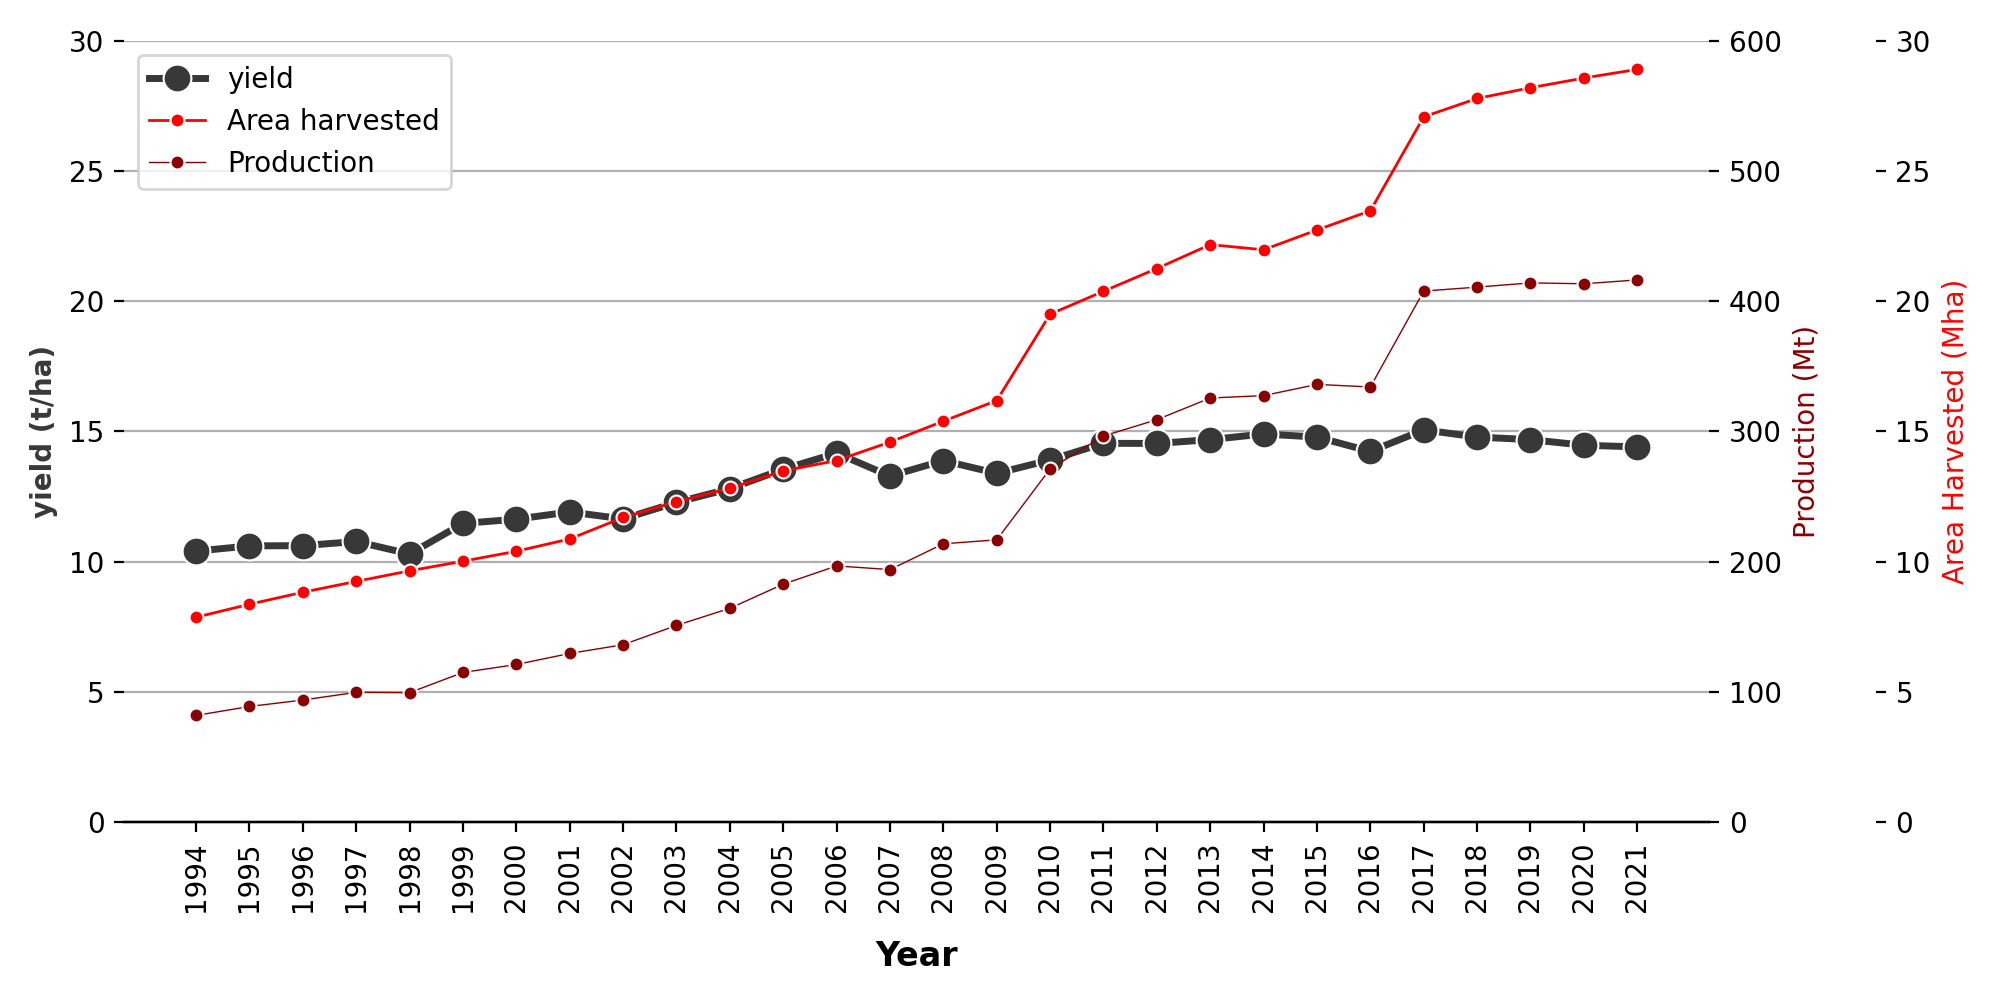
\includegraphics{text/04_literature_review_files/op_yield.png}

}

\caption{\label{fig-op_yield}Global harvest area and production of oil
palm evolve accordingly, with no yield improvement since 2011
(\protect\hyperlink{ref-faoFAOSTATDatabase2023}{FAO, 2023}).}

\end{figure}

In summary, oil palm is an essential crop globally, known for its
efficiency and high yields in tropical regions. While it has contributed
significantly to economic growth, its expansion has come at the cost of
deforestation and pollution, posing challenges to biodiversity and
ecosystems. Nonetheless, markets will continue to thrive, requiring new
solutions to reduce land use change and innovations in processing.

\hypertarget{sec-rspo}{%
\section{Labels for sustainable palm oil}\label{sec-rspo}}

Growing concern about the significant forest loss and ecosystem
degradation caused by deforestation has brought cultivation of palm oil
to public attention. As a result, the Roundtable on Sustainable Palm Oil
(RSPO) was established in 2004 to build a market for certified
sustainable palm oil by establishing environmental and social standards
for palm oil production
(\protect\hyperlink{ref-abdulmajidSustainablePalmOil2021}{Abdul Majid et
al., 2021}; \protect\hyperlink{ref-rspoWhoWeAre2023}{RSPO, 2023}). The
RSPO is formed by producers, retailers, investors and social and
environmental NGOs, with currently over 5000 members
(\protect\hyperlink{ref-rspoWhoWeAre2023}{RSPO, 2023}). With a share of
19\% on the oil palm market
(\protect\hyperlink{ref-ritchiePalmOil2021}{Ritchie, 2021}), it is
almost exclusively the only certification standard in global palm oil
trade (\protect\hyperlink{ref-murphyOilPalm2020s2021}{Murphy et al.,
2021}). Other labels such as the Malaysian Sustainable Palm Oil (MSPO)
and the Indonesian Sustainable Palm Oil (ISPO) have little to no share
in international markets and focus mainly on smallholders
(\protect\hyperlink{ref-murphyOilPalm2020s2021}{Murphy et al., 2021}).
RSPO states that compliance with its standards can mitigate the negative
impacts of palm oil production on the environment and local communities
(\protect\hyperlink{ref-rspoWhoWeAre2023}{2023}). Since 2005 RSPO
demands that new plantations must not replace primary forest and a High
Conservation Values (HCV) assessment is required for certification,
which besides ecological factors, also considers a wide range of social
stakeholders, including local communities
(\protect\hyperlink{ref-murphyOilPalm2020s2021}{Murphy et al., 2021}).
Since 2018, a High Carbon Stock (HCS) report is additionally required,
which prohibits clearing for oil palm on HCS classified lands for
certification
(\protect\hyperlink{ref-rspoRSPOPrinciplesCriteria2018}{RSPO, 2018}).
Despite public discussion on oil palm, a study on Swiss consumers
showed, that only 9\% of the participants were even aware of the RSPO
label (\protect\hyperlink{ref-wassmannPalmOilRoundtable2023}{Wassmann et
al., 2023}).

A major criticism, however, is that if forests are not classified as HCV
or HCS RSPO certifications continue to allow logging
(\protect\hyperlink{ref-cazzollagattiSustainablePalmOil2019}{Cazzolla
Gatti et al., 2019}). In addition, significant tree losses were reported
prior to and post-certification
(\protect\hyperlink{ref-cazzollagattiSustainablePalmOil2019}{Cazzolla
Gatti et al., 2019}). Furthermore, deforestation rates in certified
areas are comparable to or even exceed those in uncertified areas,
leading Cazzolla Gatti et al.~to conclude that sustainable palm oil may
not be sustainable
(\protect\hyperlink{ref-cazzollagattiSustainablePalmOil2019}{2019}). The
criticism from non-governmental organizations is even more staggering.
They claim that RSPO auditors commit numerous violations in the
licensing process, such as failing to identify indigenous land rights
claims, faulty HCV assessments or serious labor abuses
(\protect\hyperlink{ref-eiaWhoWatchesWatchmen2015}{EIA, 2015};
\protect\hyperlink{ref-greenpeaceinternationalCertifyingDestruction2013}{Greenpeace
International, 2013}).

\hypertarget{sec-infrastructure}{%
\section{Infrastructure}\label{sec-infrastructure}}

Expansion of infrastructure is happening at a high rate across the
globe. In the last two decades, the amount of built-up land area has
increased by 47\%, whereby this rate is even higher in Asia at 73\%
(\protect\hyperlink{ref-potapovGlobal20002020Land2022}{Potapov et al.,
2022}). With an additional 25 million kilometers of paved roads and more
than 300,000 kilometers of rail track, translating into a 60\% expansion
of land transportation infrastructure by 2050 compared to 2010,
infrastructure development will continue at a rapid rate
(\protect\hyperlink{ref-ieaGlobalLandTransport2013}{IEA, 2013};
\protect\hyperlink{ref-lauranceGlobalStrategyRoad2014}{Laurance et al.,
2014}). It is estimated that 90\% of this growth will take place in
developing countries projecting enormous consequences for Borneo
(\protect\hyperlink{ref-lauranceGlobalStrategyRoad2014}{Laurance et al.,
2014}).

With deforestation and infrastructure development in remote areas,
hunting pressure is intensifying
(\protect\hyperlink{ref-kamyabElaeisGuineensis2022}{Kamyab, 2022}), as
well as poaching with improved accessibility
(\protect\hyperlink{ref-mooreAreRangerPatrols2018}{Moore et al., 2018}).
In addition, the expansion of habitation of humans stimulated by
infrastructure developments is leading to an increase in human-wildlife
conflicts (\protect\hyperlink{ref-kamyabElaeisGuineensis2022}{Kamyab,
2022}).

Not only does new infrastructure increase settlement and thus human
density but it is also associated with greater dispersal pressure of
invasive species, leading to new corridors such as roads or rail tracks
that facilitate their introduction
(\protect\hyperlink{ref-darRoadsActCorridors2015}{Dar et al., 2015};
\protect\hyperlink{ref-mungiRoleSpeciesRichness2021}{Mungi et al.,
2021}). Moreover, the resulting increase in light pollution affects the
behavior of individual animal species, which in turn can influence their
ecosystem services, eventually leading to effects of land erosion
(\protect\hyperlink{ref-lewanzikArtificialLightPuts2014}{Lewanzik \&
Voigt, 2014}).

Since large parts of Borneo are covered with forest, new infrastructure
projects cut through these areas, separating and isolating large
interconnected habitats
(\protect\hyperlink{ref-alamgirHighriskInfrastructureProjects2019}{Alamgir
et al., 2019}) and enhancing deforestation nearby
(\protect\hyperlink{ref-meijerGlobalPatternsCurrent2018}{Meijer et al.,
2018};
\protect\hyperlink{ref-sloanHiddenChallengesConservation2019}{Sloan et
al., 2019}). Although ecologists agree that habitat loss has
far-reaching and detrimental consequences for biodiversity (see
Section~\ref{sec-deforestation}, Section~\ref{sec-oilpalm}), there is
disagreement about the impact that fragmentation itself has
(\protect\hyperlink{ref-didhamRethinkingConceptualFoundations2012a}{Didham
et al., 2012};
\protect\hyperlink{ref-fahrigRethinkingPatchSize2013}{Fahrig, 2013};
\protect\hyperlink{ref-haddadHabitatFragmentationIts2015a}{Haddad et
al., 2015};
\protect\hyperlink{ref-miller-rushingHowDoesHabitat2019}{Miller-Rushing
et al., 2019}). Observational studies often focused only on single
aspects of fragmentation (e.g., edge, isolation, area) and failed to
take in the full context of the complex interconnected structures of
habitats
(\protect\hyperlink{ref-haddadHabitatFragmentationIts2015a}{Haddad et
al., 2015}). However, a comprehensive experiment indicated, that
biodiversity in fragmented habitats is reduced from 13\% up to 75\%
(\protect\hyperlink{ref-haddadHabitatFragmentationIts2015a}{Haddad et
al., 2015}). More recently, Püttker et al.~underlined that biodiversity
of forest-dependent animal and, to an even greater extent, plant species
are negatively affected by habitat fragmentation, especially through
edge effects
(\protect\hyperlink{ref-puttkerIndirectEffectsHabitat2020}{2020}). This
also applies to Borneo, as many infrastructure projects, including the
planned relocation of the Indonesian capital
(\protect\hyperlink{ref-lyonsWhyIndonesiaMoving2019}{Lyons, 2019}), are
estimated to have huge impacts on biodiversity
(\protect\hyperlink{ref-alamgirHighriskInfrastructureProjects2019}{Alamgir
et al., 2019}).

To sum up, the expansion of infrastructure contributes not only to
habitat loss, but also to increased habitat isolation due to
fragmentation, increased introduction of invasive species, and light
pollution, disturbing the fauna.

\hypertarget{other-crops}{%
\section{Other crops}\label{other-crops}}

While some studies say that besides oil palm, which accounts for 88\% of
industrial plantations, pulp wood is the only crop to cover the other
12\% (\protect\hyperlink{ref-gaveauRiseFallForest2019}{Gaveau et al.,
2019}). However, other studies report that groundnut and coconut are
also grown in Borneo, but not in the from of industrial plantations
(\protect\hyperlink{ref-meijaardCoconutOilConservation2020}{Meijaard et
al., 2020}). Coconut plantations occur mainly in smallholder form
(\textless4ha) and thus
(\protect\hyperlink{ref-meijaardCoconutOilConservation2020}{Meijaard et
al., 2020}), make it challenging to map with remote sensing methods
(\protect\hyperlink{ref-descalsHighresolutionGlobalMap2021}{Descals et
al., 2021}). However, it is thought to have almost a fivefold worse
impact on biodiversity
(\protect\hyperlink{ref-meijaardCoconutOilConservation2020}{Meijaard et
al., 2020}), These results, though, have caused a lot of controversy
(\protect\hyperlink{ref-rochmyaningsihClaimThatCoconut2020}{Rochmyaningsih,
2020}).

In Southeast Asia, the total cropland extent (excluding perennial woody
crops) saw only moderate growth. While 172.9 Mha were permanently used
as cropland between 2000 and 2003, 184.5 Mha were used between 2016 and
2019 (\protect\hyperlink{ref-potapovGlobalMapsCropland2021}{Potapov et
al., 2021}). A gain of 30.9 Mha offsetted a reduction of 19.3 Mha
(\protect\hyperlink{ref-potapovGlobalMapsCropland2021}{Potapov et al.,
2021}). Nevertheless, due to public awareness and the rapid expansion of
harvest area, oil palm has been extensively researched and mapped
(\protect\hyperlink{ref-descalsHighresolutionGlobalMap2021}{Descals et
al., 2021}), while maps on other crops harvest area distribution are
still sparse
(\protect\hyperlink{ref-meijaardCoconutOilConservation2020}{Meijaard et
al., 2020}).

In summary, due to much smaller expansion of cropland and perennial
woody crops, oil palm diminishes the importance of research on other
crops in Southeast Asia and thus there are hardly any maps available
making use of the advances in remotely sensed data processing (see
Section~\ref{sec-remotesensing}).

\hypertarget{sec-remotesensing}{%
\section{Advances in remote sensing}\label{sec-remotesensing}}

Since the launch of the Landsat-1 MSS satellite in 1972, an increasingly
comprehensive time series database has been built as newly launched
satellites have been equipped with more advanced technology
(\protect\hyperlink{ref-crowleyRemoteSensingRecent2020}{Crowley \&
Cardille, 2020}). However, it was not until 2008 that this data was made
available through the free and open Landsat data policy
(\protect\hyperlink{ref-zhuBenefitsFreeOpen2019}{Zhu et al., 2019}).
Combined with the launch of the European Space Agency's open-access
Copernicus mission, research from satellite data has exploded in recent
years (\protect\hyperlink{ref-crowleyRemoteSensingRecent2020}{Crowley \&
Cardille, 2020}; \protect\hyperlink{ref-zhuBenefitsFreeOpen2019}{Zhu et
al., 2019}). This development has also been facilitated by the
availability of massive-throughput analysis platforms like the Google
Earth Engine implemented in 2010
(\protect\hyperlink{ref-crowleyRemoteSensingRecent2020}{Crowley \&
Cardille, 2020}). Another crucial achievement was the development of
machine learning algorithms that separates the remotely sensed data into
meaningful classifications
(\protect\hyperlink{ref-crowleyRemoteSensingRecent2020}{Crowley \&
Cardille, 2020}). Furthermore, machine learning offers unprecedented
potential for gaining deeper insights from historical data, as well as
filling in gaps in it
(\protect\hyperlink{ref-sarafanovMachineLearningApproach2020}{Sarafanov
et al., 2020}).

Despite these advancements, many high-resolution land cover and land use
(LCLU) datasets
(\protect\hyperlink{ref-descalsHighresolutionGlobalMap2021}{Descals et
al., 2021}; \protect\hyperlink{ref-karraGlobalLandUse2021}{Karra et al.,
2021}; \protect\hyperlink{ref-zanagaESAWorldCover102021}{Zanaga et al.,
2021}), while offering unprecedented detail, do not support
multi-decadal analysis
(\protect\hyperlink{ref-potapovGlobal20002020Land2022}{Potapov et al.,
2022}). However, medium resolution (30m resolution) multidecadal
datasets are more widely available
(\protect\hyperlink{ref-danyloMapExtentYear2021}{Danylo et al., 2021};
\protect\hyperlink{ref-hansenHighResolutionGlobalMaps2013}{Hansen et
al., 2013};
\protect\hyperlink{ref-potapovGlobal20002020Land2022}{Potapov et al.,
2022}, \protect\hyperlink{ref-potapovGlobalMapsCropland2021}{2021};
\protect\hyperlink{ref-turubanovaOngoingPrimaryForest2018}{Turubanova et
al., 2018};
\protect\hyperlink{ref-tyukavinaGlobalTrendsForest2022}{Tyukavina et
al., 2022}).

\bookmarksetup{startatroot}

\hypertarget{sec-method}{%
\chapter{Materials and Method}\label{sec-method}}

\hypertarget{data-acquisition-and-selection}{%
\section{Data acquisition and
selection}\label{data-acquisition-and-selection}}

Initially, databases such as Web of Knowledge or Google Scholar were
searched for GIS and remote sensing studies covering the extent Borneo
or Southeast Asia. However, most of the studies that provide the
necessary data have been carried out on a global scale. The exerts of
the datasets covering Borneo were downloaded and visualized in QGIS
(Version 3.30) for initial data exploration. This led to the manual
selection of data presented in Figure~\ref{fig-data_overview} for the
subsequent analysis. Hereafter, the datasets are referred to by the
names specified in the content column. All raster datasets were in tif
format and the vector data in shapefile format. The research area was
defined as the landmass of Borneo, excluding the smaller surrounding
islands. This delineation was obtained through the download of the
Borneon boundary using the OSMnx python package (Verison 1.3.0), which
accesses the Open Street Maps (OSM) database
(\protect\hyperlink{ref-boeingOSMnxPythonPackage2017}{Boeing, 2017}).

\begin{figure}

{\centering 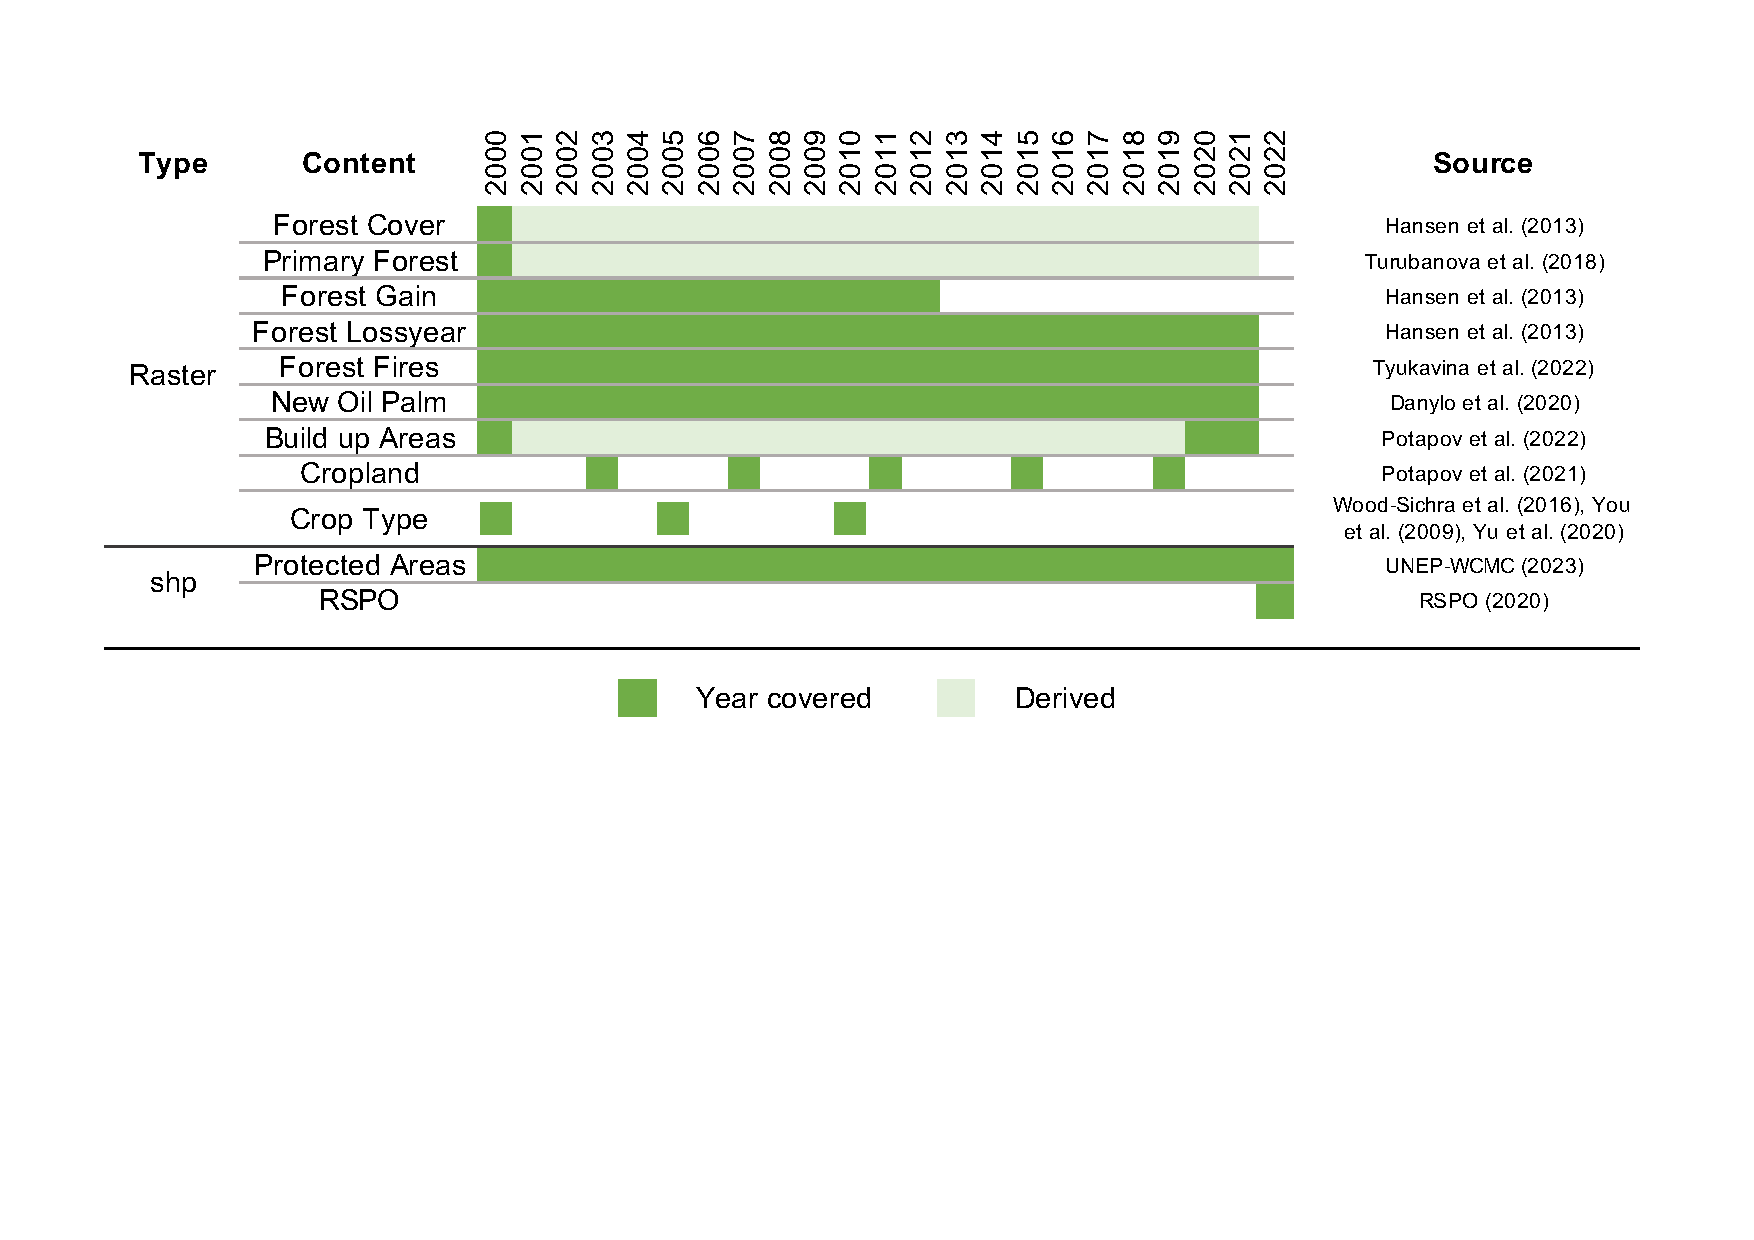
\includegraphics{text/05_method_files/data_overview.pdf}

}

\caption{\label{fig-data_overview}All datasets used in this thesis and
the temporal scope they span.}

\end{figure}

Forest cover shows the percent of closed canopy in the year 2000 of
vegetation higher than 5m
(\protect\hyperlink{ref-hansenHighResolutionGlobalMaps2013}{Hansen et
al., 2013}). Turubanov et al.~used expert-interpreted training data for
detection of patterns recognized as primary forest
(\protect\hyperlink{ref-turubanovaOngoingPrimaryForest2018}{2018}). The
forest loss shows the year of quick changes in forest cover to
\textasciitilde0\% closed canopy
(\protect\hyperlink{ref-hansenHighResolutionGlobalMaps2013}{Hansen et
al., 2013}). Forest fires show the forest loss in the joint extent of
the forest loss area by Hansen et al.
(\protect\hyperlink{ref-hansenHighResolutionGlobalMaps2013}{2013};
\protect\hyperlink{ref-tyukavinaGlobalTrendsForest2022}{Tyukavina et
al., 2022}). New oil palms shows the year they were detected for the
span 1984 - 2017 (\protect\hyperlink{ref-danyloMapExtentYear2021}{Danylo
et al., 2021}). Oil palms are detected no earlier than 4 years after
planting (\protect\hyperlink{ref-danyloMapExtentYear2021}{Danylo et al.,
2021}). The built up areas dataset contains two categories: i) built up
areas in 2000 and ii) newly built up areas between 2001 and 2020
(\protect\hyperlink{ref-potapovGlobal20002020Land2022}{Potapov et al.,
2022}). The cropland datasets shows land used for agriculture where
shrubby plants were consistently cultivated over four years. Even though
multiple spatial datasets allocate crop type spatially, none of them is
based on remotely sensed data
(\protect\hyperlink{ref-groganGlobalGriddedCrop2022}{Grogan et al.,
2022};
\protect\hyperlink{ref-wood-sichraSpatialProductionAllocation2016}{Wood-Sichra
et al., 2016}; \protect\hyperlink{ref-youMappingGlobalCropping2022}{You
\& Sun, 2022};
\protect\hyperlink{ref-youGeneratingPlausibleCrop2009}{You et al.,
2009}; \protect\hyperlink{ref-yuCultivatedPlanet20102020}{Yu et al.,
2020}). The Spatial Production Allocation Model (SPAM) takes the most
factors into account rendering it the most comprehensive data. The data
shows harvest area of multiple crops within a 5 arcminute
(\textasciitilde8km) resolution. Protected areas represent those
registered in the World Database on Protected Areas
(\protect\hyperlink{ref-unep-wcmcProtectedAreaProfile2023}{UNEP-WCMC,
2023}). Although the RSPO stated in early 2020 that the RSPO concessions
will also be made publicly available for Indonesia
(\protect\hyperlink{ref-rspoRSPOMEMBERSCONCESSION2020}{RSPO, 2020}),
this is still not the case as of today. A personal inquiry about this
also remained unanswered. Thus, analysis of RSPO concessions could only
be carried out for Malaysia. The Borneon and Malaysian boundaries are
both derived from OpenStreetMap.

\hypertarget{software}{%
\section{Software}\label{software}}

All data preparation and analysis steps were performed using open-source
Python packages in Visual Studio Code (Version 1.83.0). Python version
was 3.10.9. Rasterio (Version 1.3.6) and NumPy (Version 1.24.3) were the
most relevant packages for data processing
(\protect\hyperlink{ref-gilliesRasterioDocumentation2023}{Gillies,
2023}; \protect\hyperlink{ref-harrisArrayProgrammingNumPy2020}{Harris et
al., 2020}). A comprehensive user-friendly set of functions was created.
These functions require one or multiple input paths, an output path and
optionally a reference file path (e.g.~a mask tif, snap tif, etc.) and
addtional conditions (e.g.~mask values). The output file was compressed
in lzw form. The full code is available on
\href{https://github.com/pfaffrob/03_vs_code}{github.com/pfaffrob/03\_vs\_code}.
OpenAI's Chat-GPT (versions 3.0, 3.5 and 4.0) was used to support code
generation. Functions were developed by starting with a minimal example
with aid of Chat-GPT. Subsequently, more complex features were
implemented into the function through personal adjustments or continuous
user feedback to the AI. The generated code and its output files were
carefully inspected to ensure correctness.

\hypertarget{data-preparation}{%
\section{Data preparation}\label{data-preparation}}

For area calculations, it is crucial to choose a well-suited coordinate
reference system (crs). The use of one UTM zone was considered too
inaccurate since Borneo spans four UTM zones. The only crs available
covering Borneo is the Timbalai 1948
(\protect\hyperlink{ref-klokantechnologiesgmbhTimbalai1948RSO}{Klokan
Technologies GmbH, n.d.}). But even this projection only adequately
depicts the Malaysian part, and thus distorts the larger Indonesian part
of Borneo, resulting in biased results. Therefore the Lambert Azimuthal
Equal Area Projection was chosen as it is well suited to accurately
represent the area at large spatial
scales.(\protect\hyperlink{ref-esriQuick_Notes_on_Map_Projections_in_ArcGIS_nov2019Pdf2019}{esri,
2019}, \protect\hyperlink{ref-esriLambertAzimuthalEqualarea2023}{2023}).
Although this does not affect the area calculations, the origin was
manually set to the center of Borneo (115° longitude; 0° latitude) to
achieve maps of Borneo with minimal distortion.

All data has been brought into a consistent format. This required
merging, clipping, reclassification and snapping, which includes
resampling of the data with method nearest neighbour. For the latter,
the forest loss dataset was chosen as the reference grid. The workflow
for the preparation of raster and vector data is visible in
Figure~\ref{fig-data_preparation}. Preparation steps were only carried
out if it was required. For example, the datasets for primary forests
and forest fires consisted of only one file, hence there was no need for
merging.

\begin{figure}[H]

\begin{minipage}[t]{\linewidth}

{\centering 

\raisebox{-\height}{

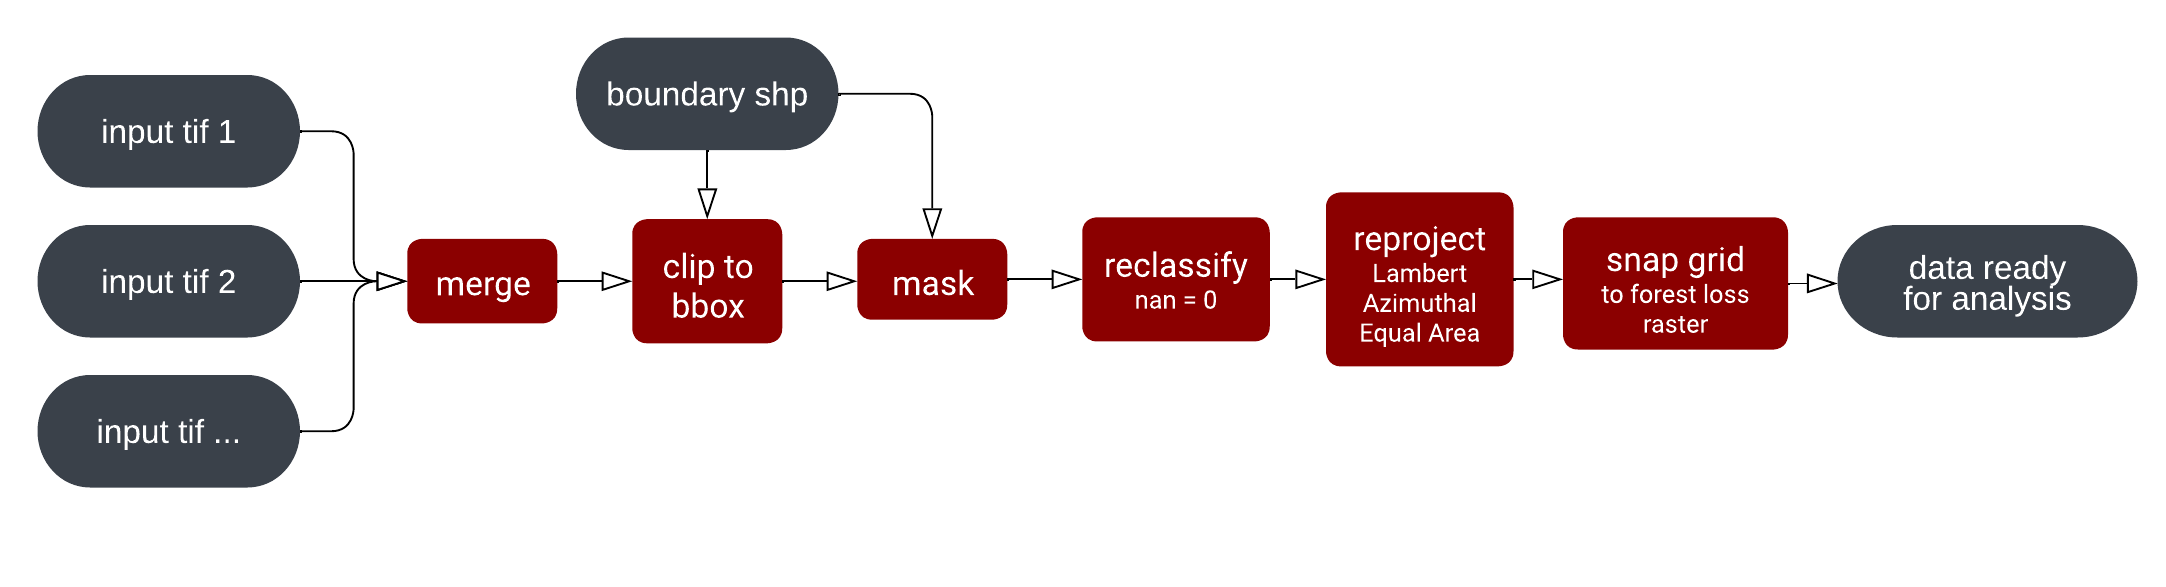
\includegraphics{text/05_method_files/raster_preparation.png}

}

}

\subcaption{\label{fig-raster_preparation}Processing steps for
preparation of raster data.}
\end{minipage}%
\newline
\begin{minipage}[t]{\linewidth}

{\centering 

\raisebox{-\height}{

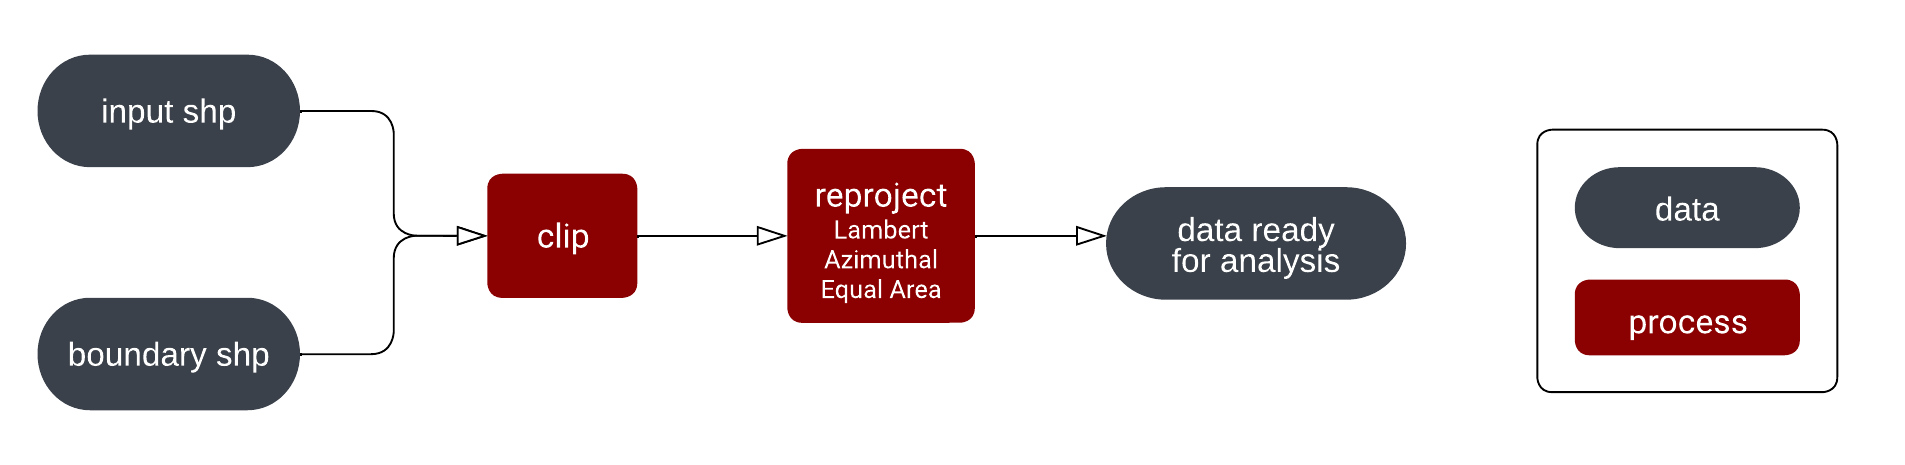
\includegraphics{text/05_method_files/shp_preparation.png}

}

}

\subcaption{\label{fig-shp_preparation}Processing steps for preparation
of shapefiles.}
\end{minipage}%

\caption{\label{fig-data_preparation}Workflow of data preparation for
raster data and \textbf{(b)} shapefiles. The steps were applied as
necessary. The legend in figure \textbf{(b)} also applies to
\textbf{(a)}.}

\end{figure}

\hypertarget{analysis}{%
\section{Analysis}\label{analysis}}

For answering the simpler questions that required only one data set,
such as quantifying annual deforestation rates or total primary forest
area in 2000, the area calculations could be performed without any
further steps. The more complex processing steps are described below.
Area calculations were performed by counting the frequency of unique
pixel values and multiplying them by the area of one pixel. The entire
maps are also presented
\href{https://storymaps.arcgis.com/stories/4594866b4f414b8aa7571325336db771}{online}.

\hypertarget{deforestation}{%
\subsection{Deforestation}\label{deforestation}}

The forest cover dataset shows the percentage of canopy cover. A
threshold of 75\% closed canopy was chosen as the definition of forest,
which was also used by Turubanova et al.~for comparison of their results
with the same forest loss data source
(\protect\hyperlink{ref-turubanovaOngoingPrimaryForest2018}{2018}).
Although areas with \textgreater75\% closed canopy overlap nearly all of
the primary forest areas (see Annex II), these were reclassified as
forest. The workflow for all forest loss-related analysis steps is shown
in Figure~\ref{fig-wf_deforestation}.

\begin{figure}[H]

{\centering 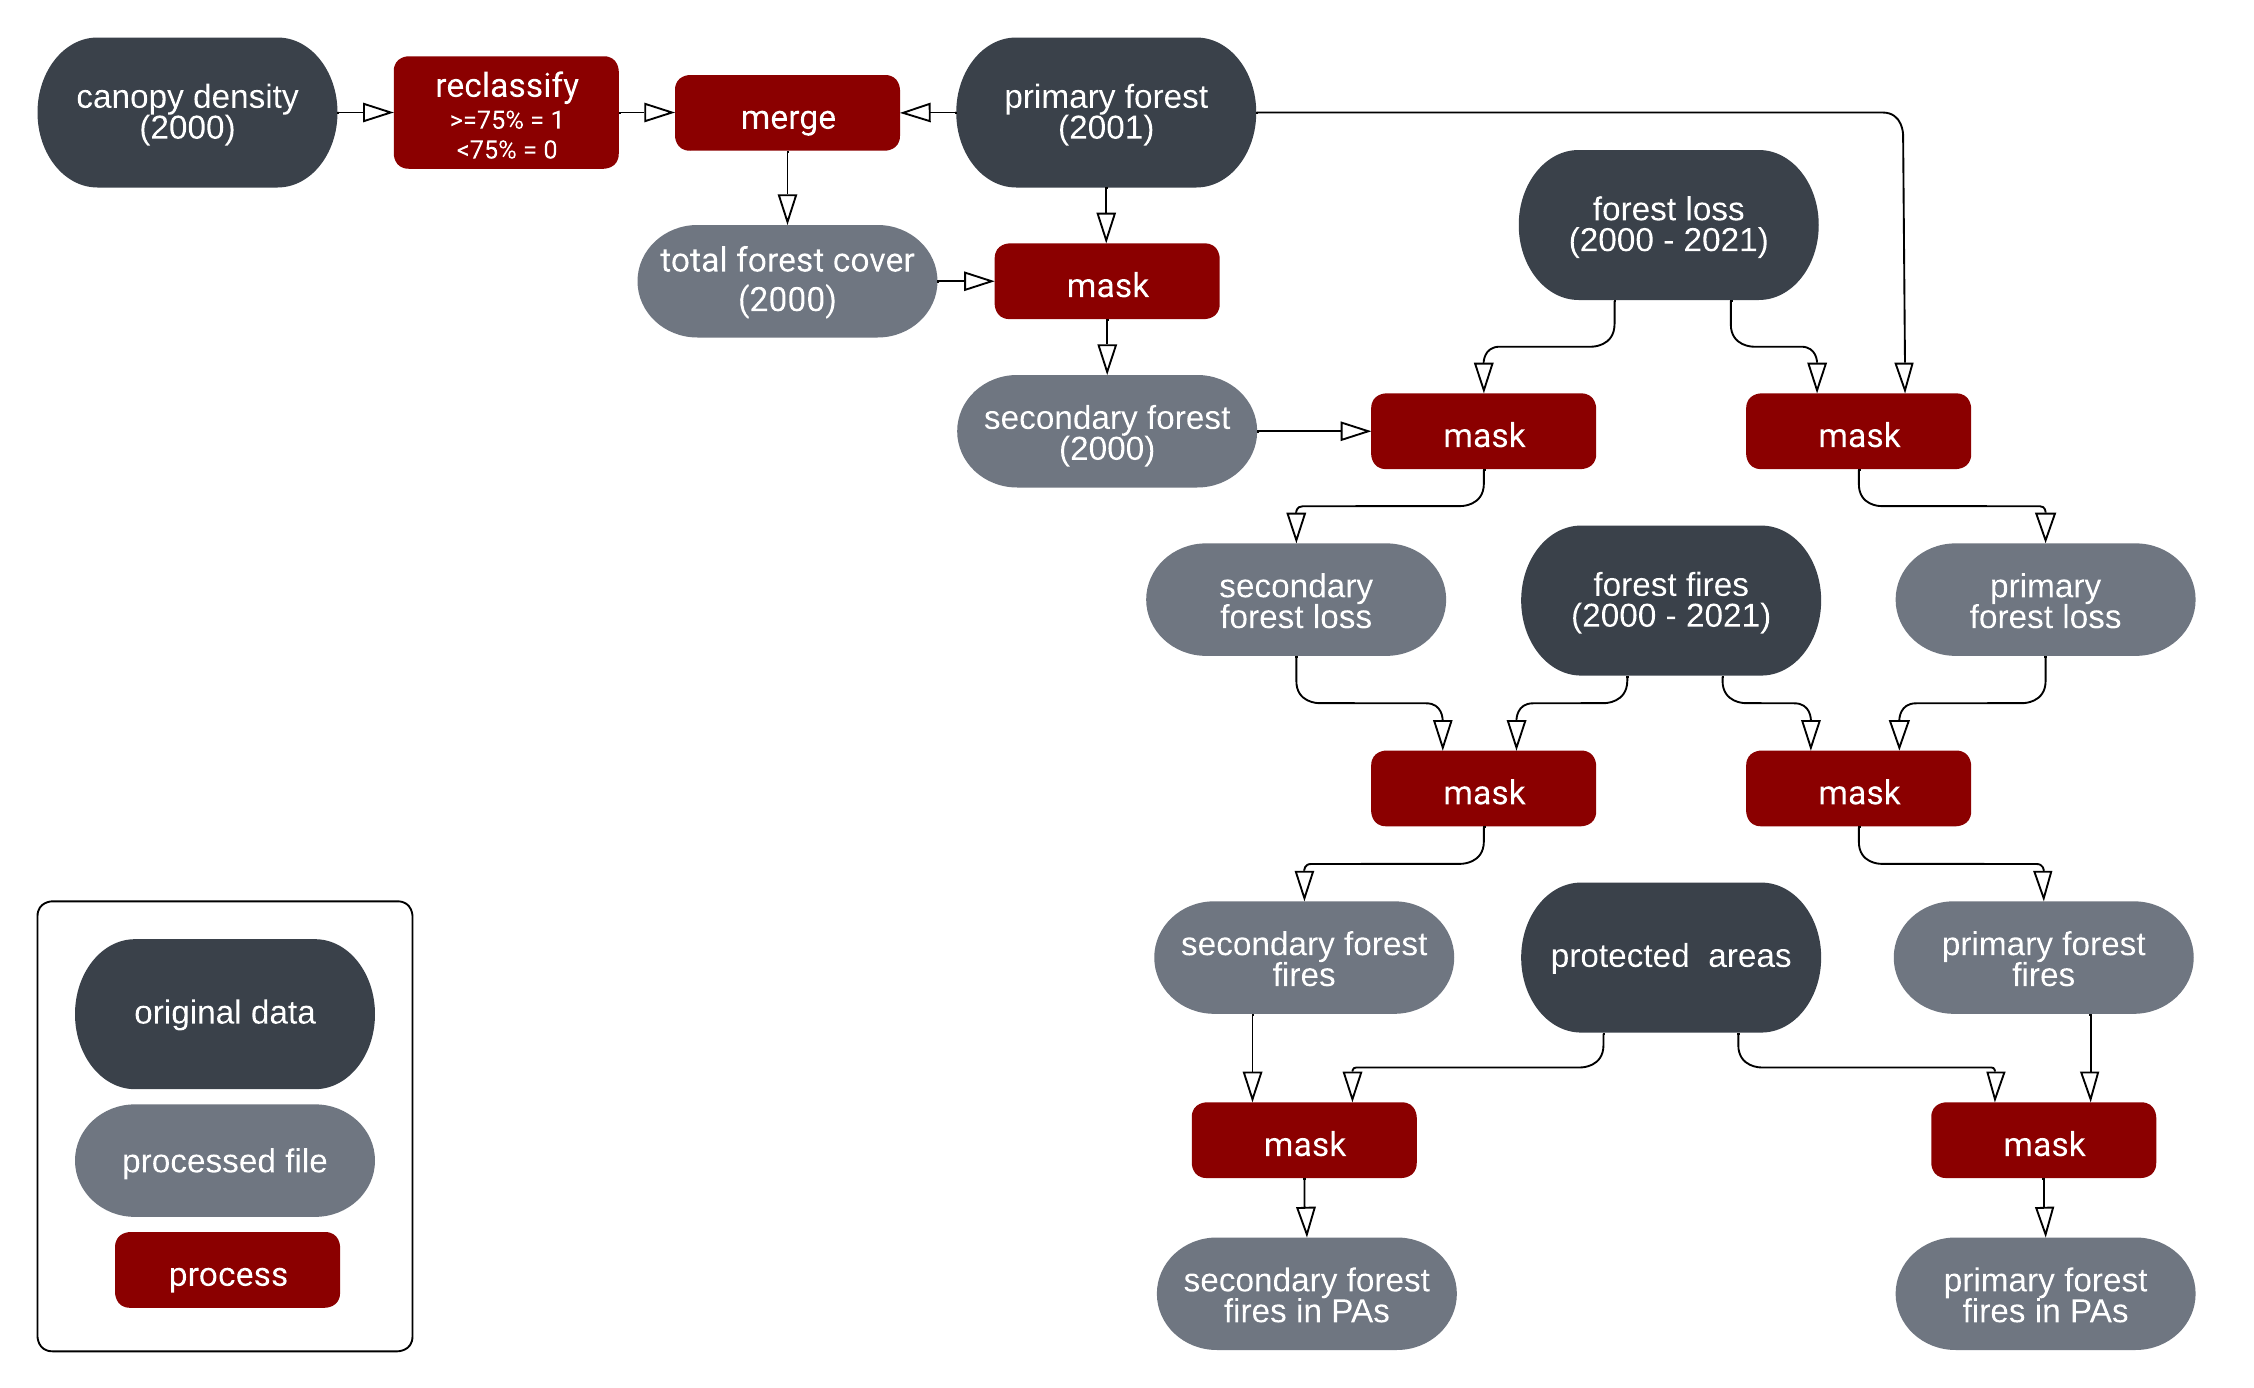
\includegraphics{text/05_method_files/wf_deforestation.png}

}

\caption{\label{fig-wf_deforestation}Workflow of deforestation
analysis.}

\end{figure}

\begin{figure}[H]

{\centering 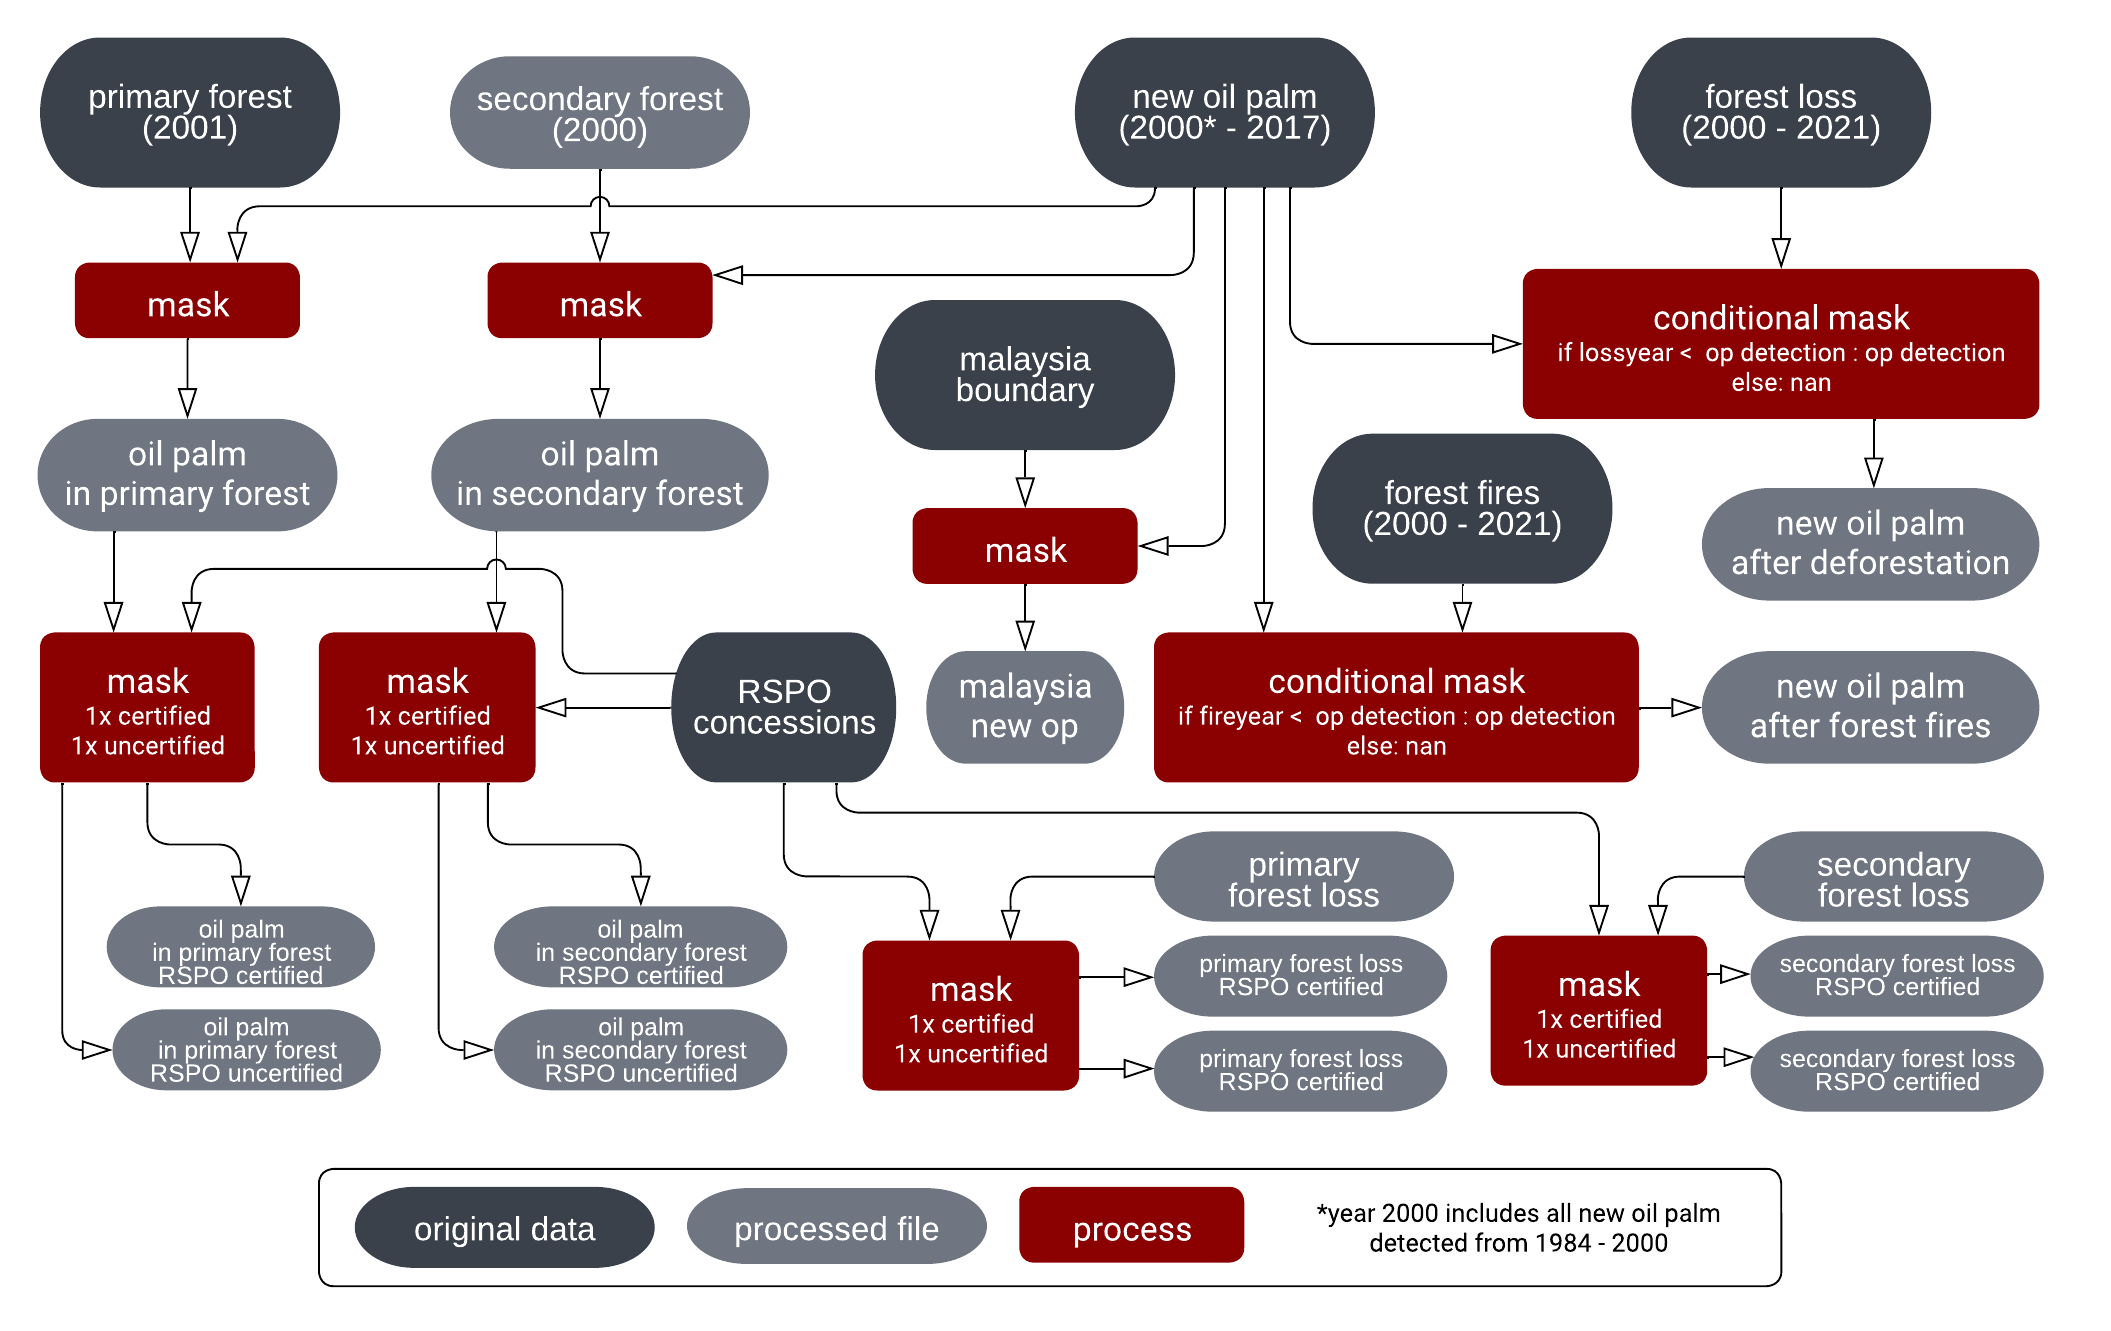
\includegraphics{text/05_method_files/op_workflow.png}

}

\caption{\label{fig-wf_oilpalm}Workflow of oil palm and RSPO
concessions.}

\end{figure}

\newpage

\hypertarget{oil-palm}{%
\subsection{Oil palm}\label{oil-palm}}

Multiple processing steps were performed using the created geoprocessing
functions for analysis of oil palm and its contribution to defrestation
(Figure~\ref{fig-wf_oilpalm}). The new oil palm dataset was already in
the preprocessing limited to the study period. RSPO primary forest loss
secondary forest loss and new oil palm plantations were analyzed for
both RSPO-certified and uncertified concessions.

\hypertarget{infrastructure}{%
\subsection{Infrastructure}\label{infrastructure}}

The processing steps for infrastructure analysis were conducted using
the geoprocessing functions. The workflow is visible in
Figure~\ref{fig-wf_infrastructure}.

\begin{figure}[H]

{\centering 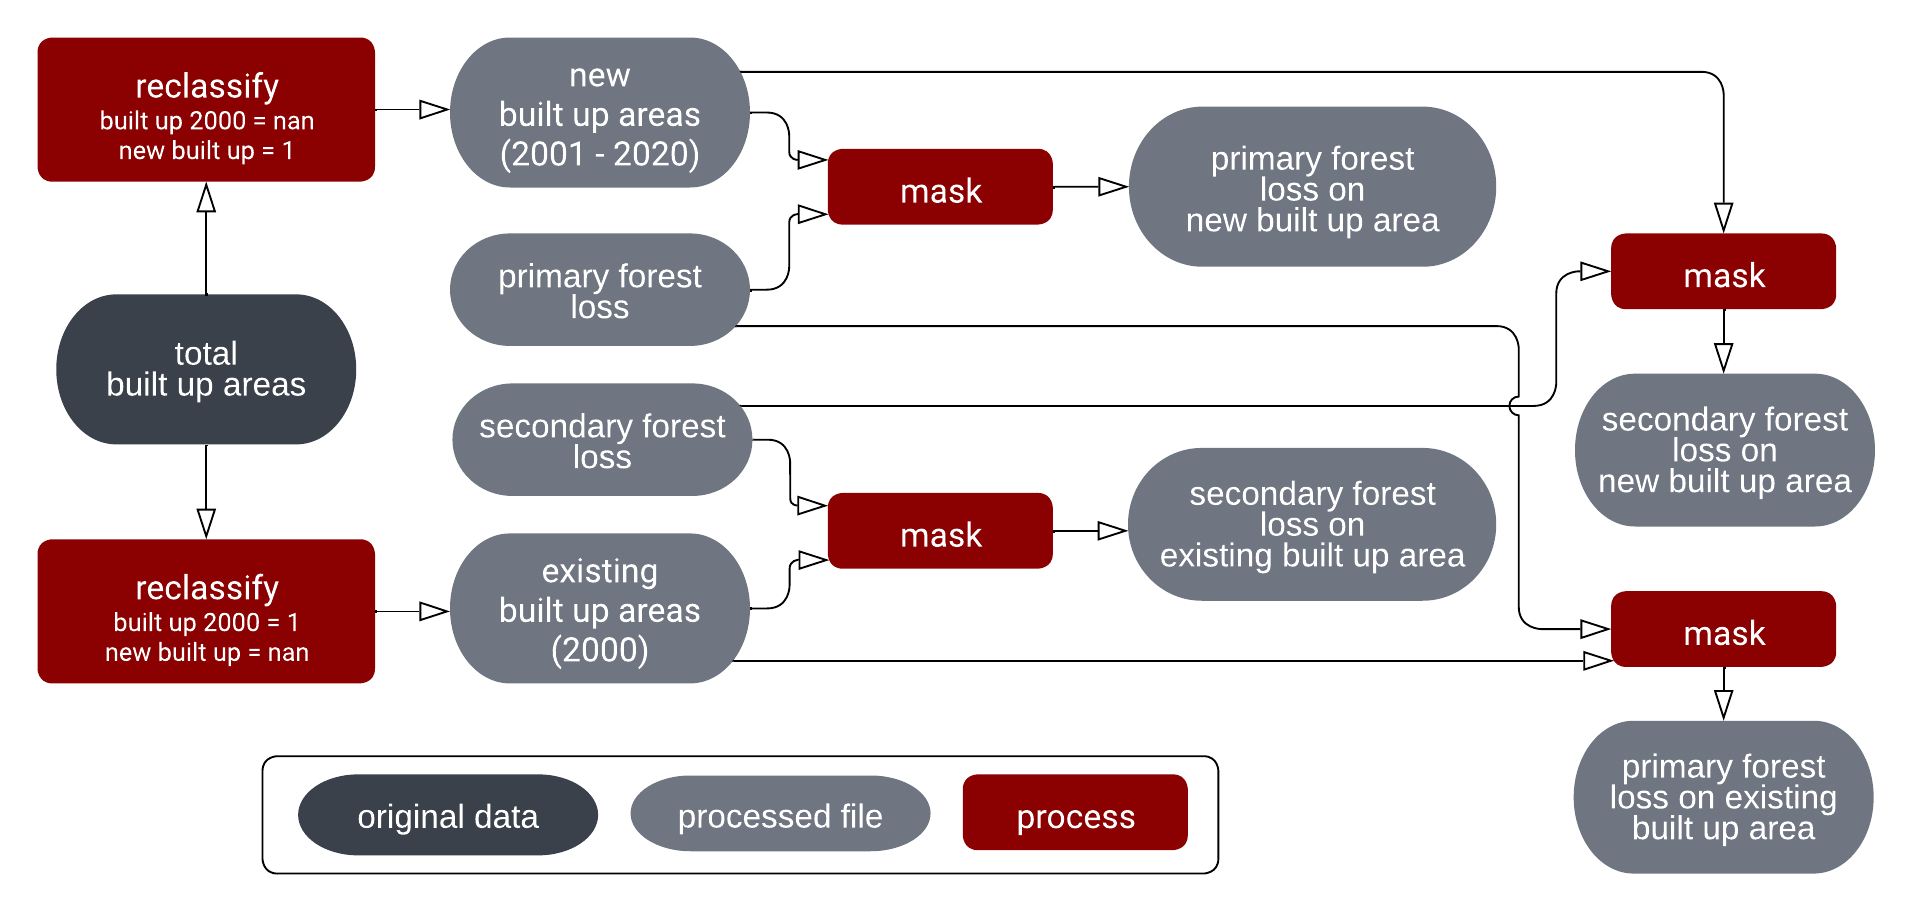
\includegraphics{text/05_method_files/wf_infrastructure.png}

}

\caption{\label{fig-wf_infrastructure}Workflow to determine
deforestation due to infrastructure.}

\end{figure}

\hypertarget{buffer-infrastructure}{%
\subsubsection{Buffer infrastructure}\label{buffer-infrastructure}}

To create buffer zones based on the built-up areas, each pixel whose
center was located within a radius of 100, 200, 500, 1000, and 2000
meters to a pixel of built up area was used as a mask for further
analysis. Existing infrastructure in 2000, new infrastructure created
from 2001 to 2020 and the total infrastructure in 2020 were each
buffered individually. The workflow of this is visible in
Figure~\ref{fig-wf_buffer}.

\begin{figure}[H]

{\centering 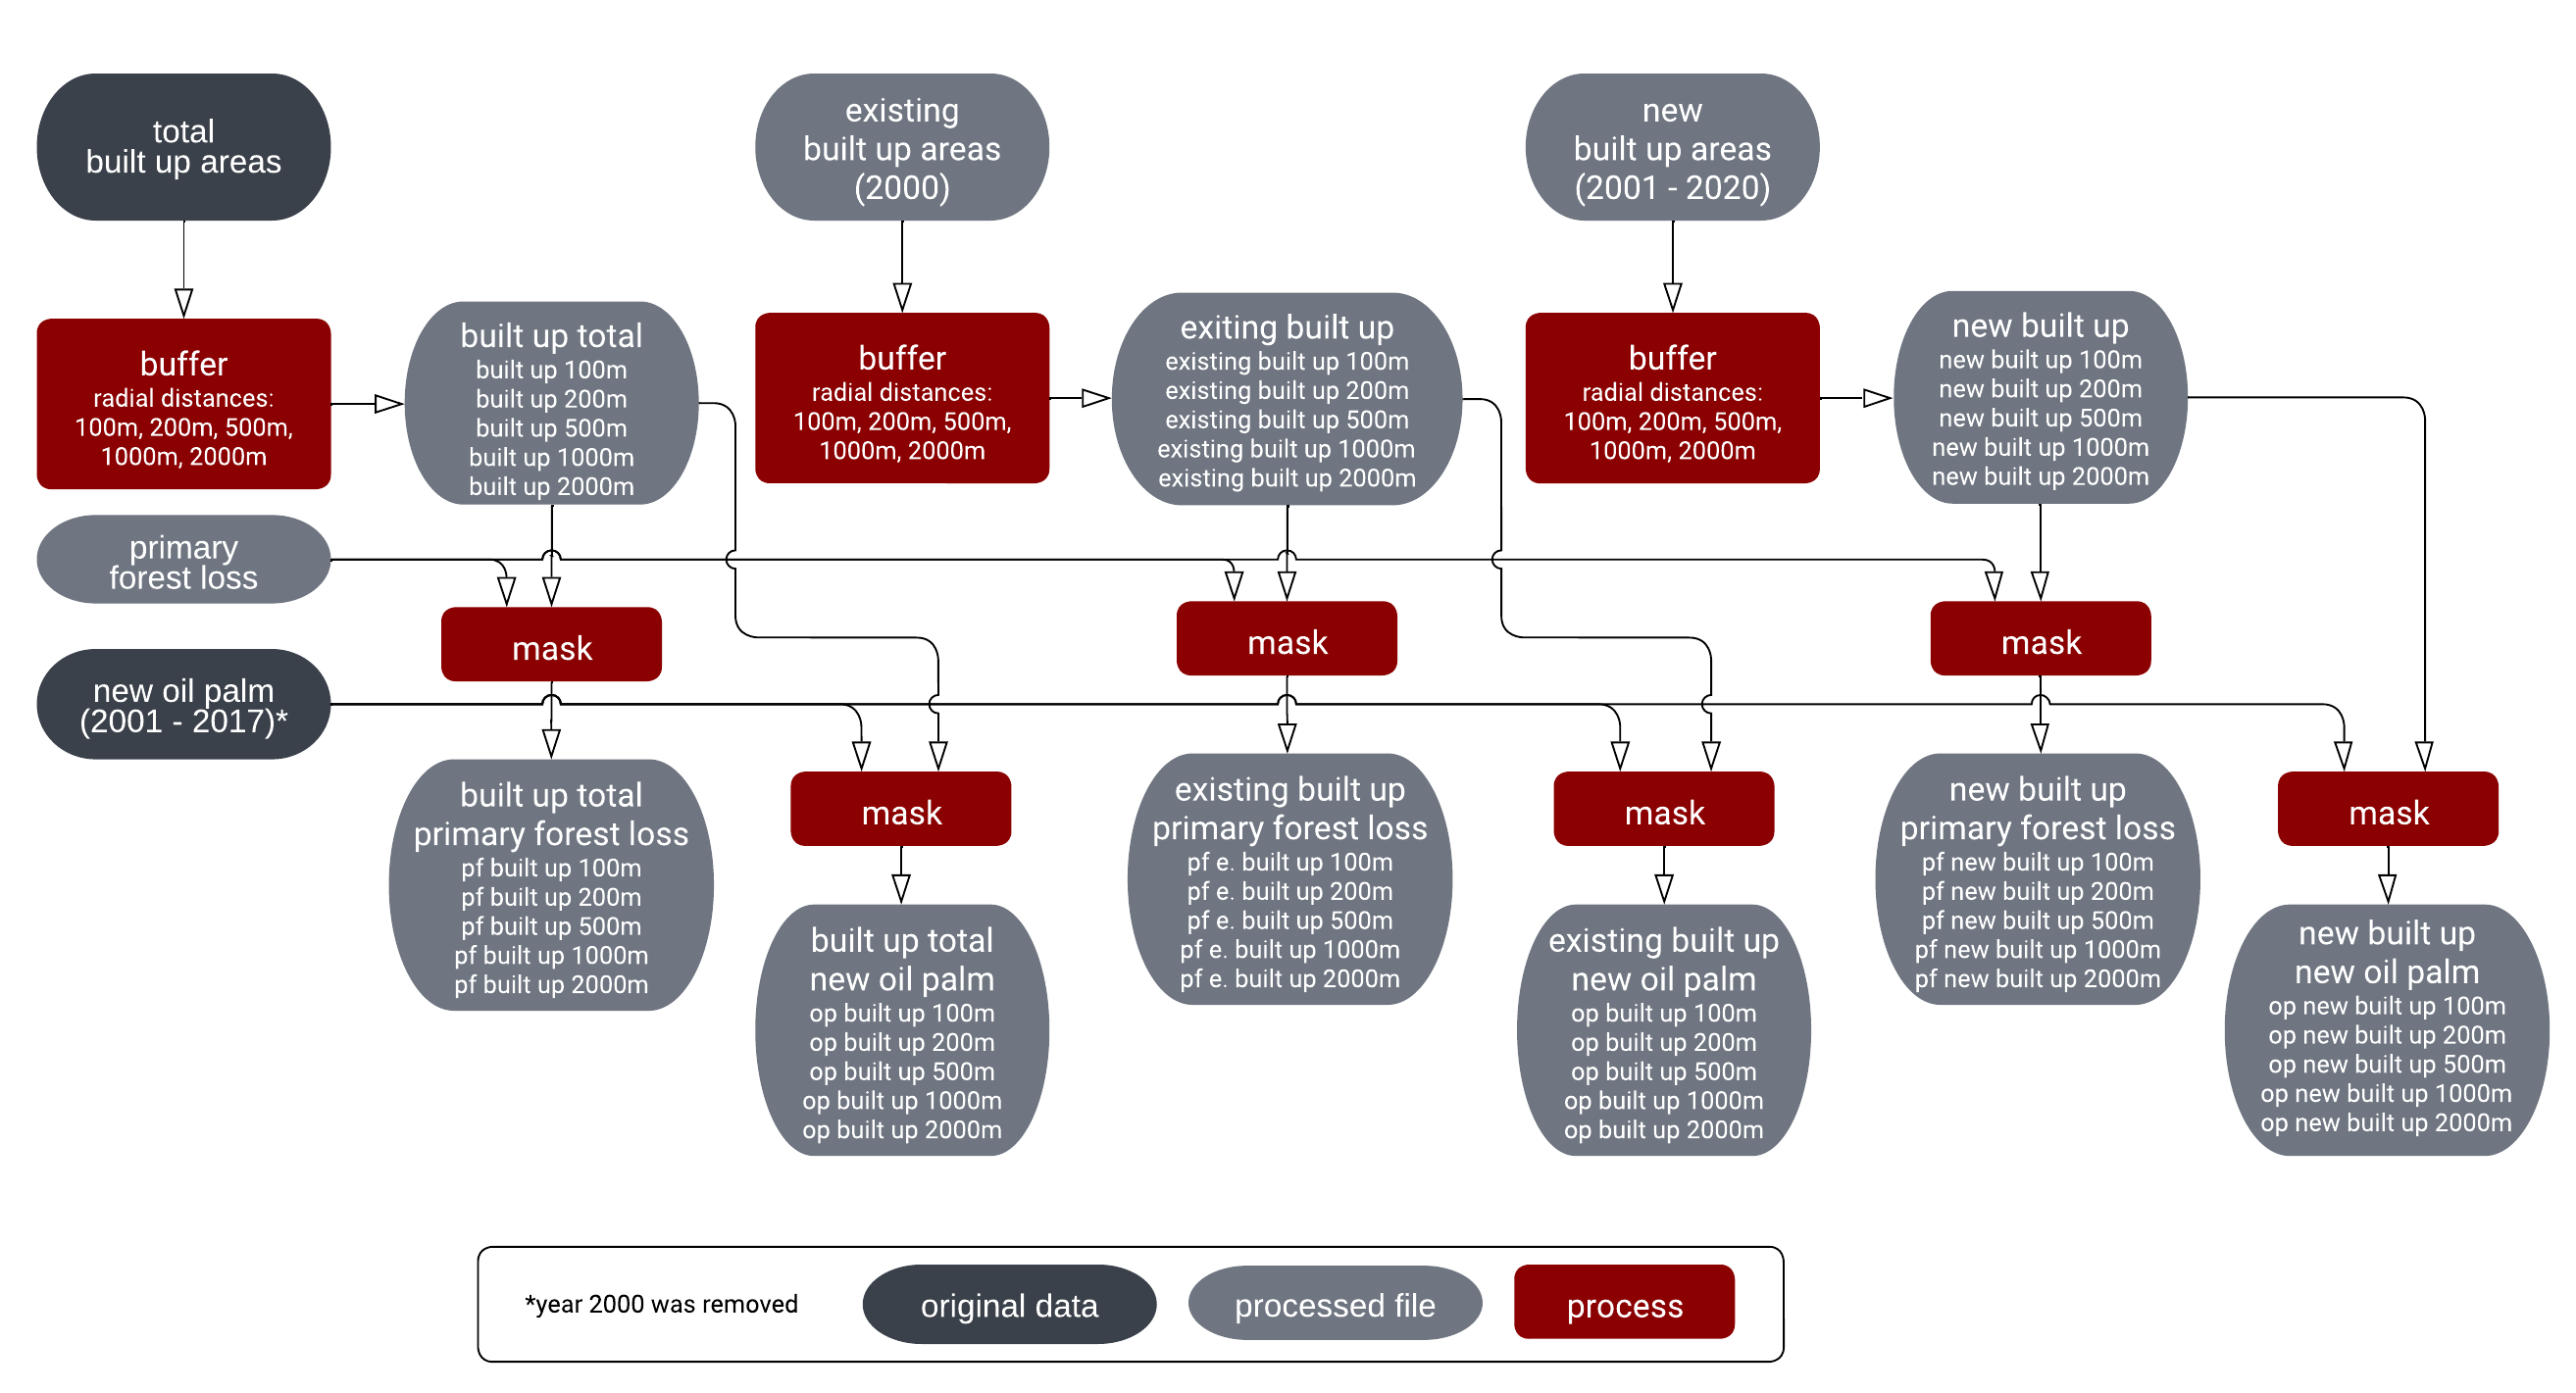
\includegraphics{text/05_method_files/wf_buffer.png}

}

\caption{\label{fig-wf_buffer}Workflow of buffer maps and subsequent
combination with other datasets}

\end{figure}

\hypertarget{other-crops-1}{%
\section{Other crops}\label{other-crops-1}}

The five cropland datasets were each masked with previous forest loss to
determine deforestation. An analysis of conversion from other crops to
oil palm and vice versa was not conducted because (i) the intersection
of cropland (at any point in time) with oil palm was considered too
small (\textgreater0.2\% of total oil palm area) and (ii) the data on
crop types proved to be inaccurate, as it was indicated that more than 1
Mha of land was used to grow non-woody crops (Annex IX), while the
remotely sensed data on uniform cropland, which should represent these
same crops, was only \textasciitilde0.2 million ha.

Open source emote sensing data is not available for other perennial
woody crops such as coconut rubber or pulpwood.

\bookmarksetup{startatroot}

\hypertarget{results}{%
\chapter{Results}\label{results}}

\hypertarget{borneo-in-2000}{%
\section{Borneo in 2000}\label{borneo-in-2000}}

At the beginning of the millennium, more than half (54.3\%) of the
island of Borneo, which has an area of 728,799 km\textsuperscript{2},
was covered with primary forests. The remaining areas were 30.4\%
covered with secondary forest, and 15.3\% in nonforest state.
Figure~\ref{fig-piefcover2000} provides an overview of the composition
of vegetation on Borneo at the start of the study period.

\begin{figure}

{\centering 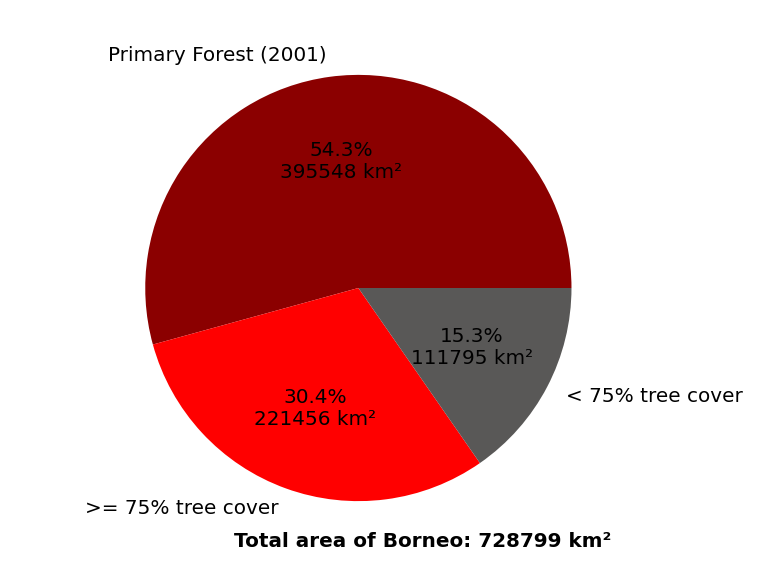
\includegraphics[width=0.6\textwidth,height=\textheight]{text/../code/results/final_plots/fcover_2000.png}

}

\caption{\label{fig-piefcover2000}Composition of vegetated areas on
Borneo at the start of the study period.}

\end{figure}

4886 km\textsuperscript{2} or 2.2\% of the secondary forest cover
represent oil palms (detection up to 2003), with a lot of these oil palm
plantations being close to typical plantation patterns (see annex IV).
Another notable characteristic are large areas of secondary forest
within primary forest close to rivers, especially with human settlements
nearby (see annex V).

\hypertarget{deforestation-1}{%
\section{Deforestation}\label{deforestation-1}}

In the years from 2001 to 2021, a total of 16.81 Mha of deforestation
occurred. 6.13 Mha of this is within primary forests and 10.68 Mha
outside of primary forests. In both, logging was mainly responsible for
forest loss, compared to forest fires. While logging rates in secondary
forests increased from 0.3 to almost 0.5 Mha per year by 2008, the five
most deforestation-intensive years, with 0.61 - 0.75 Mha of forest loss,
occurred between 2009 and 2016. After three years of steady
deforestation at 0.5 Mha per year, less than 0.4 Mha of forest loss was
recorded in 2020 and 2021 Figure~\ref{fig-bardeforestation}. Within
primary forests, logging rates increased from 0.11 Mha in 2002 to a
maximum of 0.50 in 2012 and declined back to 0.11 Mha in 2021
Figure~\ref{fig-bardeforestationprimary}. Although there was less
overall forest loss in primary forests, there were more forest fires
therein (0.81 Mha) than outside (0.72 Mha). Both primary and secondary
forests had their highest forest fire rates, by a large margin, in 2016
with 208,000 ha (secondary forest) and 255,000 ha (primary forest).
Other years with elevated forest fire rates were 2003, 2007, 2009, 2014
and 2015 ranging from 25,000 to 79,000 ha
Figure~\ref{fig-forestlossbarcharts}.

\begin{figure}

\begin{minipage}[t]{0.49\linewidth}

{\centering 

\raisebox{-\height}{

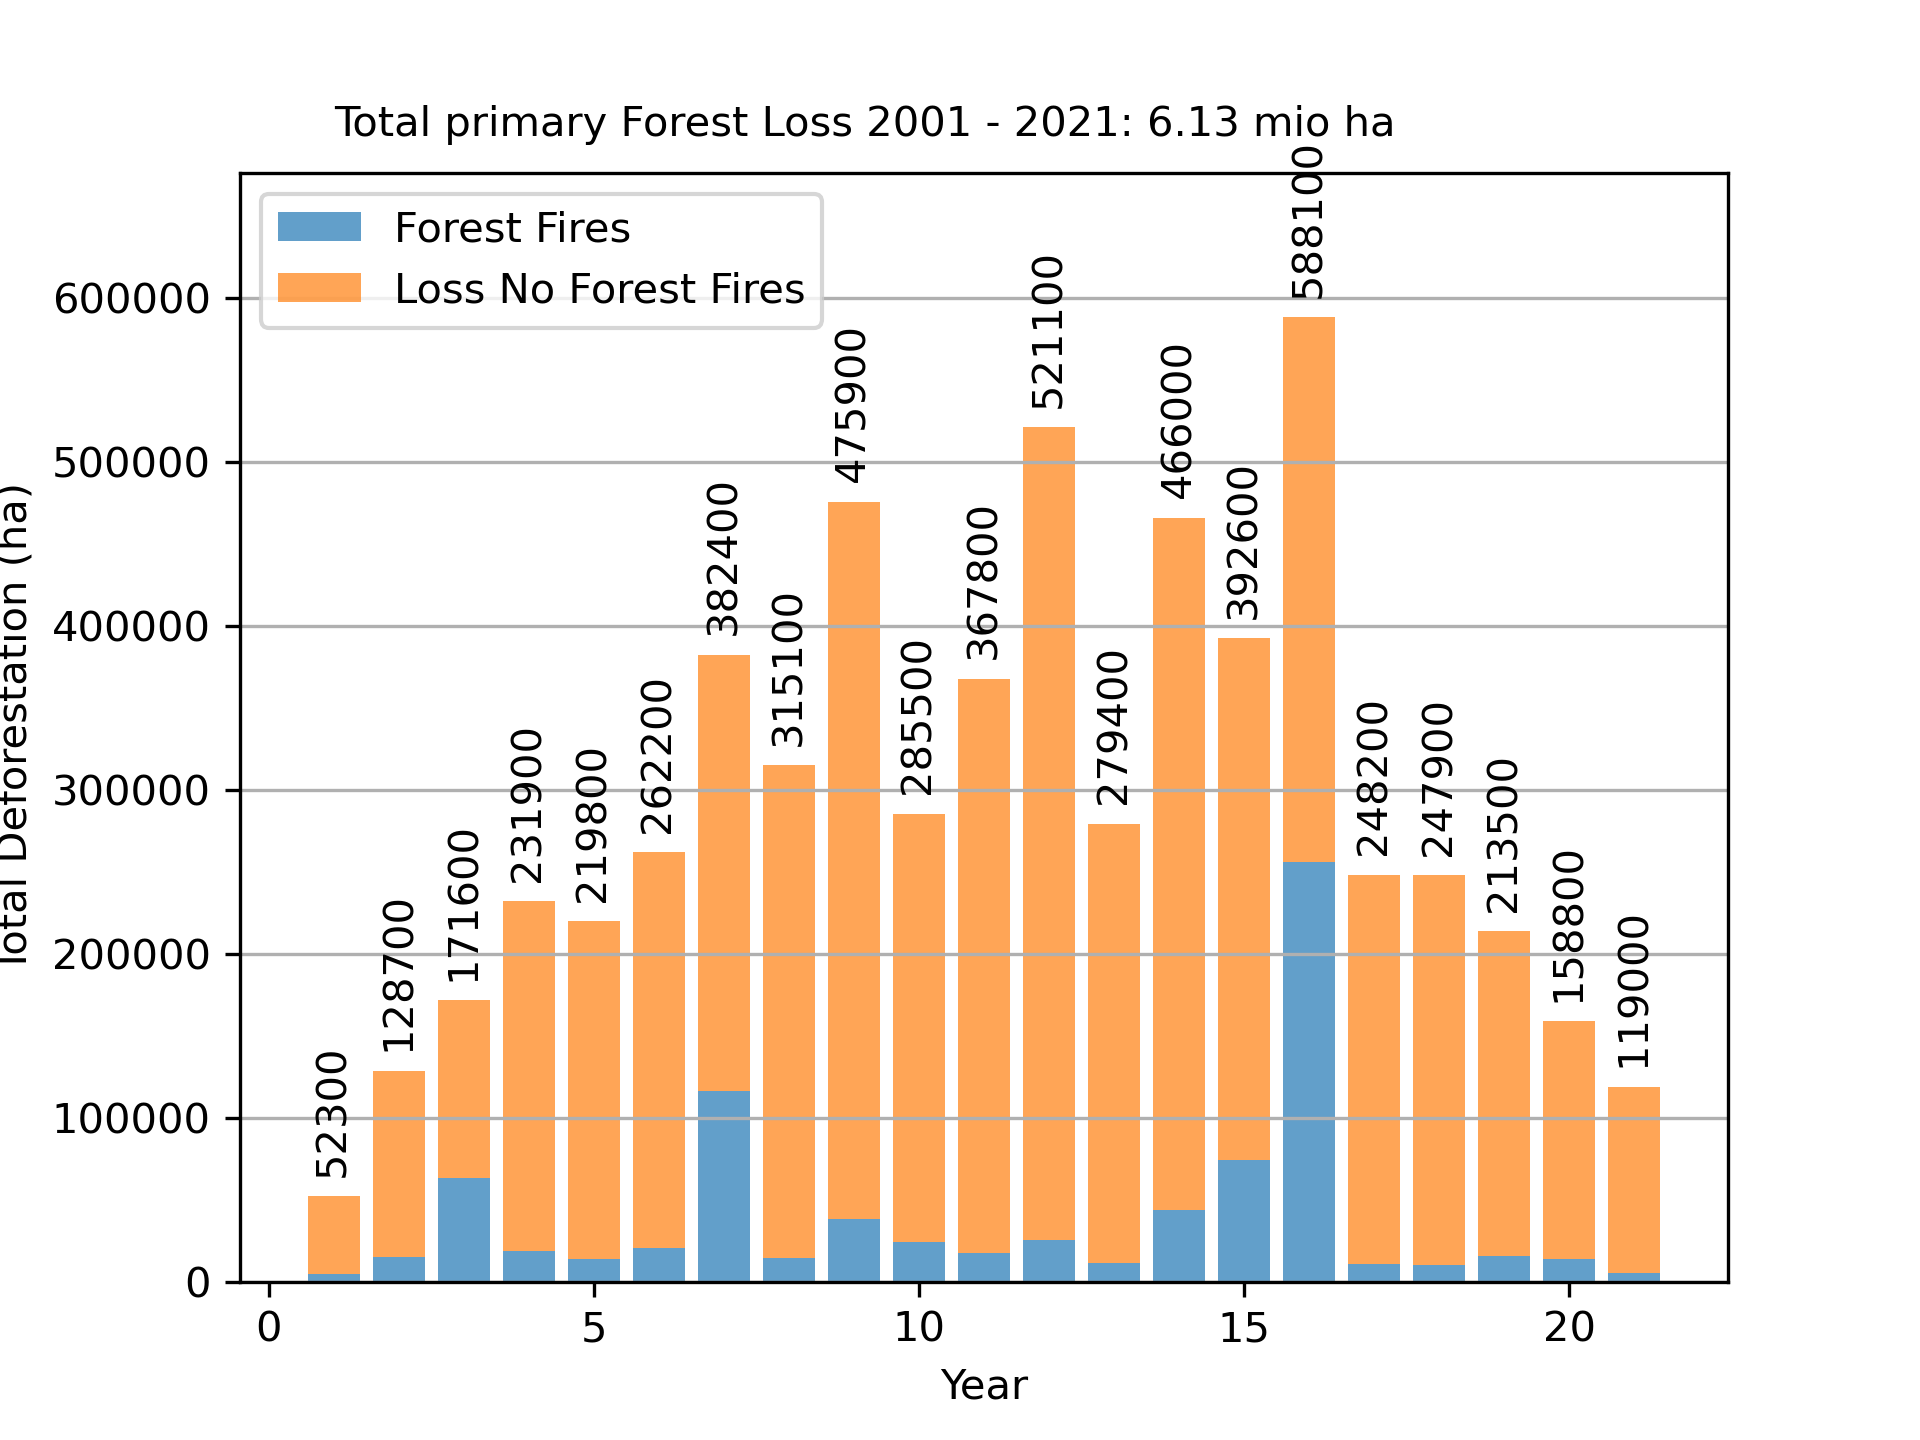
\includegraphics{text/../code/results/final_plots/total_primary_forest_deforestation.png}

}

}

\subcaption{\label{fig-bardeforestationprimary}Primary forest loss,
peaking in 2016.}
\end{minipage}%
%
\begin{minipage}[t]{0.02\linewidth}

{\centering 

~

}

\end{minipage}%
%
\begin{minipage}[t]{0.49\linewidth}

{\centering 

\raisebox{-\height}{

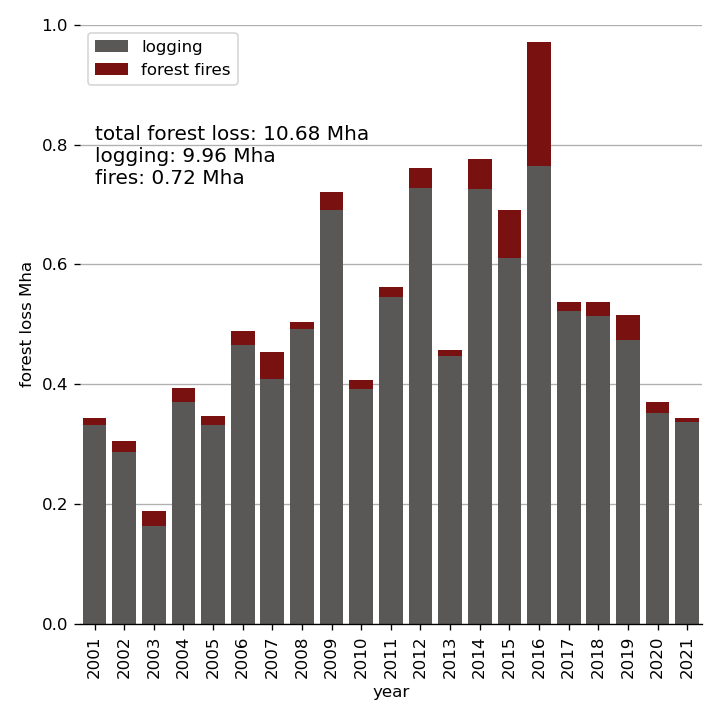
\includegraphics{text/../code/results/final_plots/total_deforestation.png}

}

}

\subcaption{\label{fig-bardeforestation}Secondary forest loss, peaking
in 2016.}
\end{minipage}%

\caption{\label{fig-forestlossbarcharts}Overview of deforestation within
\textbf{(a)} primary forests and \textbf{(b)} secondary forests.}

\end{figure}

In general, logging patterns can be separated into two categories.
First, large areas of logging in the same year, often with sharp
borders, and second, dispersed small-scale logging
(Figure~\ref{fig-map_deforestation_op_fires}, annex VI). This is
especially the case in primary forests in the Malaysian part of Borneo,
where logging continuously encroaches
(Figure~\ref{fig-map_deforestation_primary}). Fires in secondary forests
have no obvious patterns; they occur randomly and mainly on a small
scale (Figure~\ref{fig-map_deforestation_op_fires}).

\begin{figure}[H]

\begin{minipage}[t]{0.49\linewidth}

{\centering 

\raisebox{-\height}{

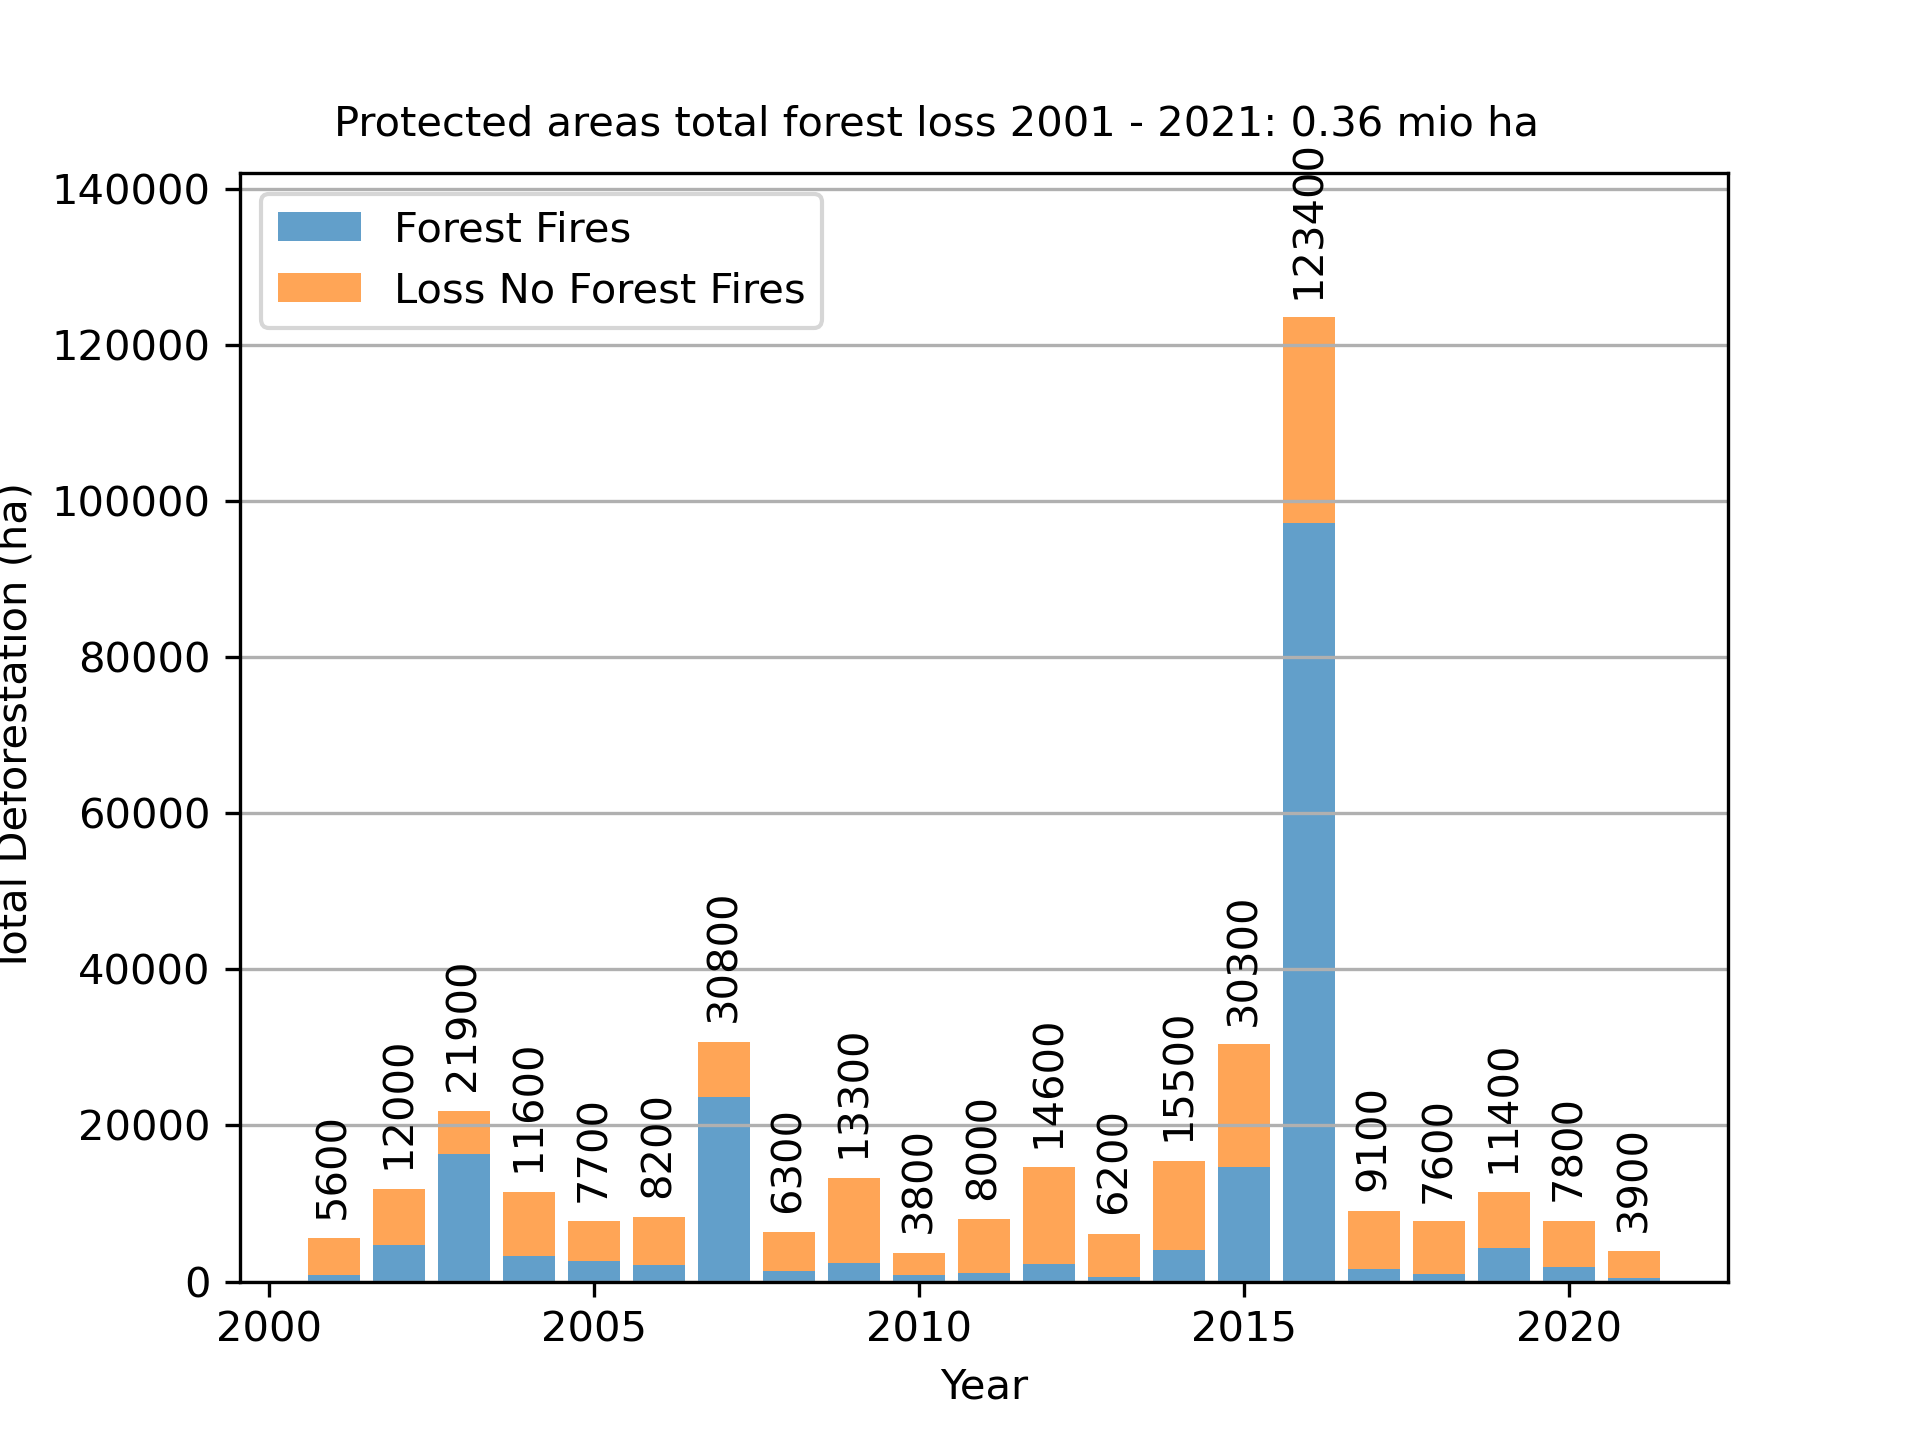
\includegraphics{text/../code/results/final_plots/deforestation_protected_areas.png}

}

}

\subcaption{\label{fig-bardeforestationprotected}Annual rates of primary
forest loss within protected areas. The total area of primary forest in
these areas is 4.72 Mha.}
\end{minipage}%
%
\begin{minipage}[t]{0.02\linewidth}

{\centering 

~

}

\end{minipage}%
%
\begin{minipage}[t]{0.49\linewidth}

{\centering 

\raisebox{-\height}{

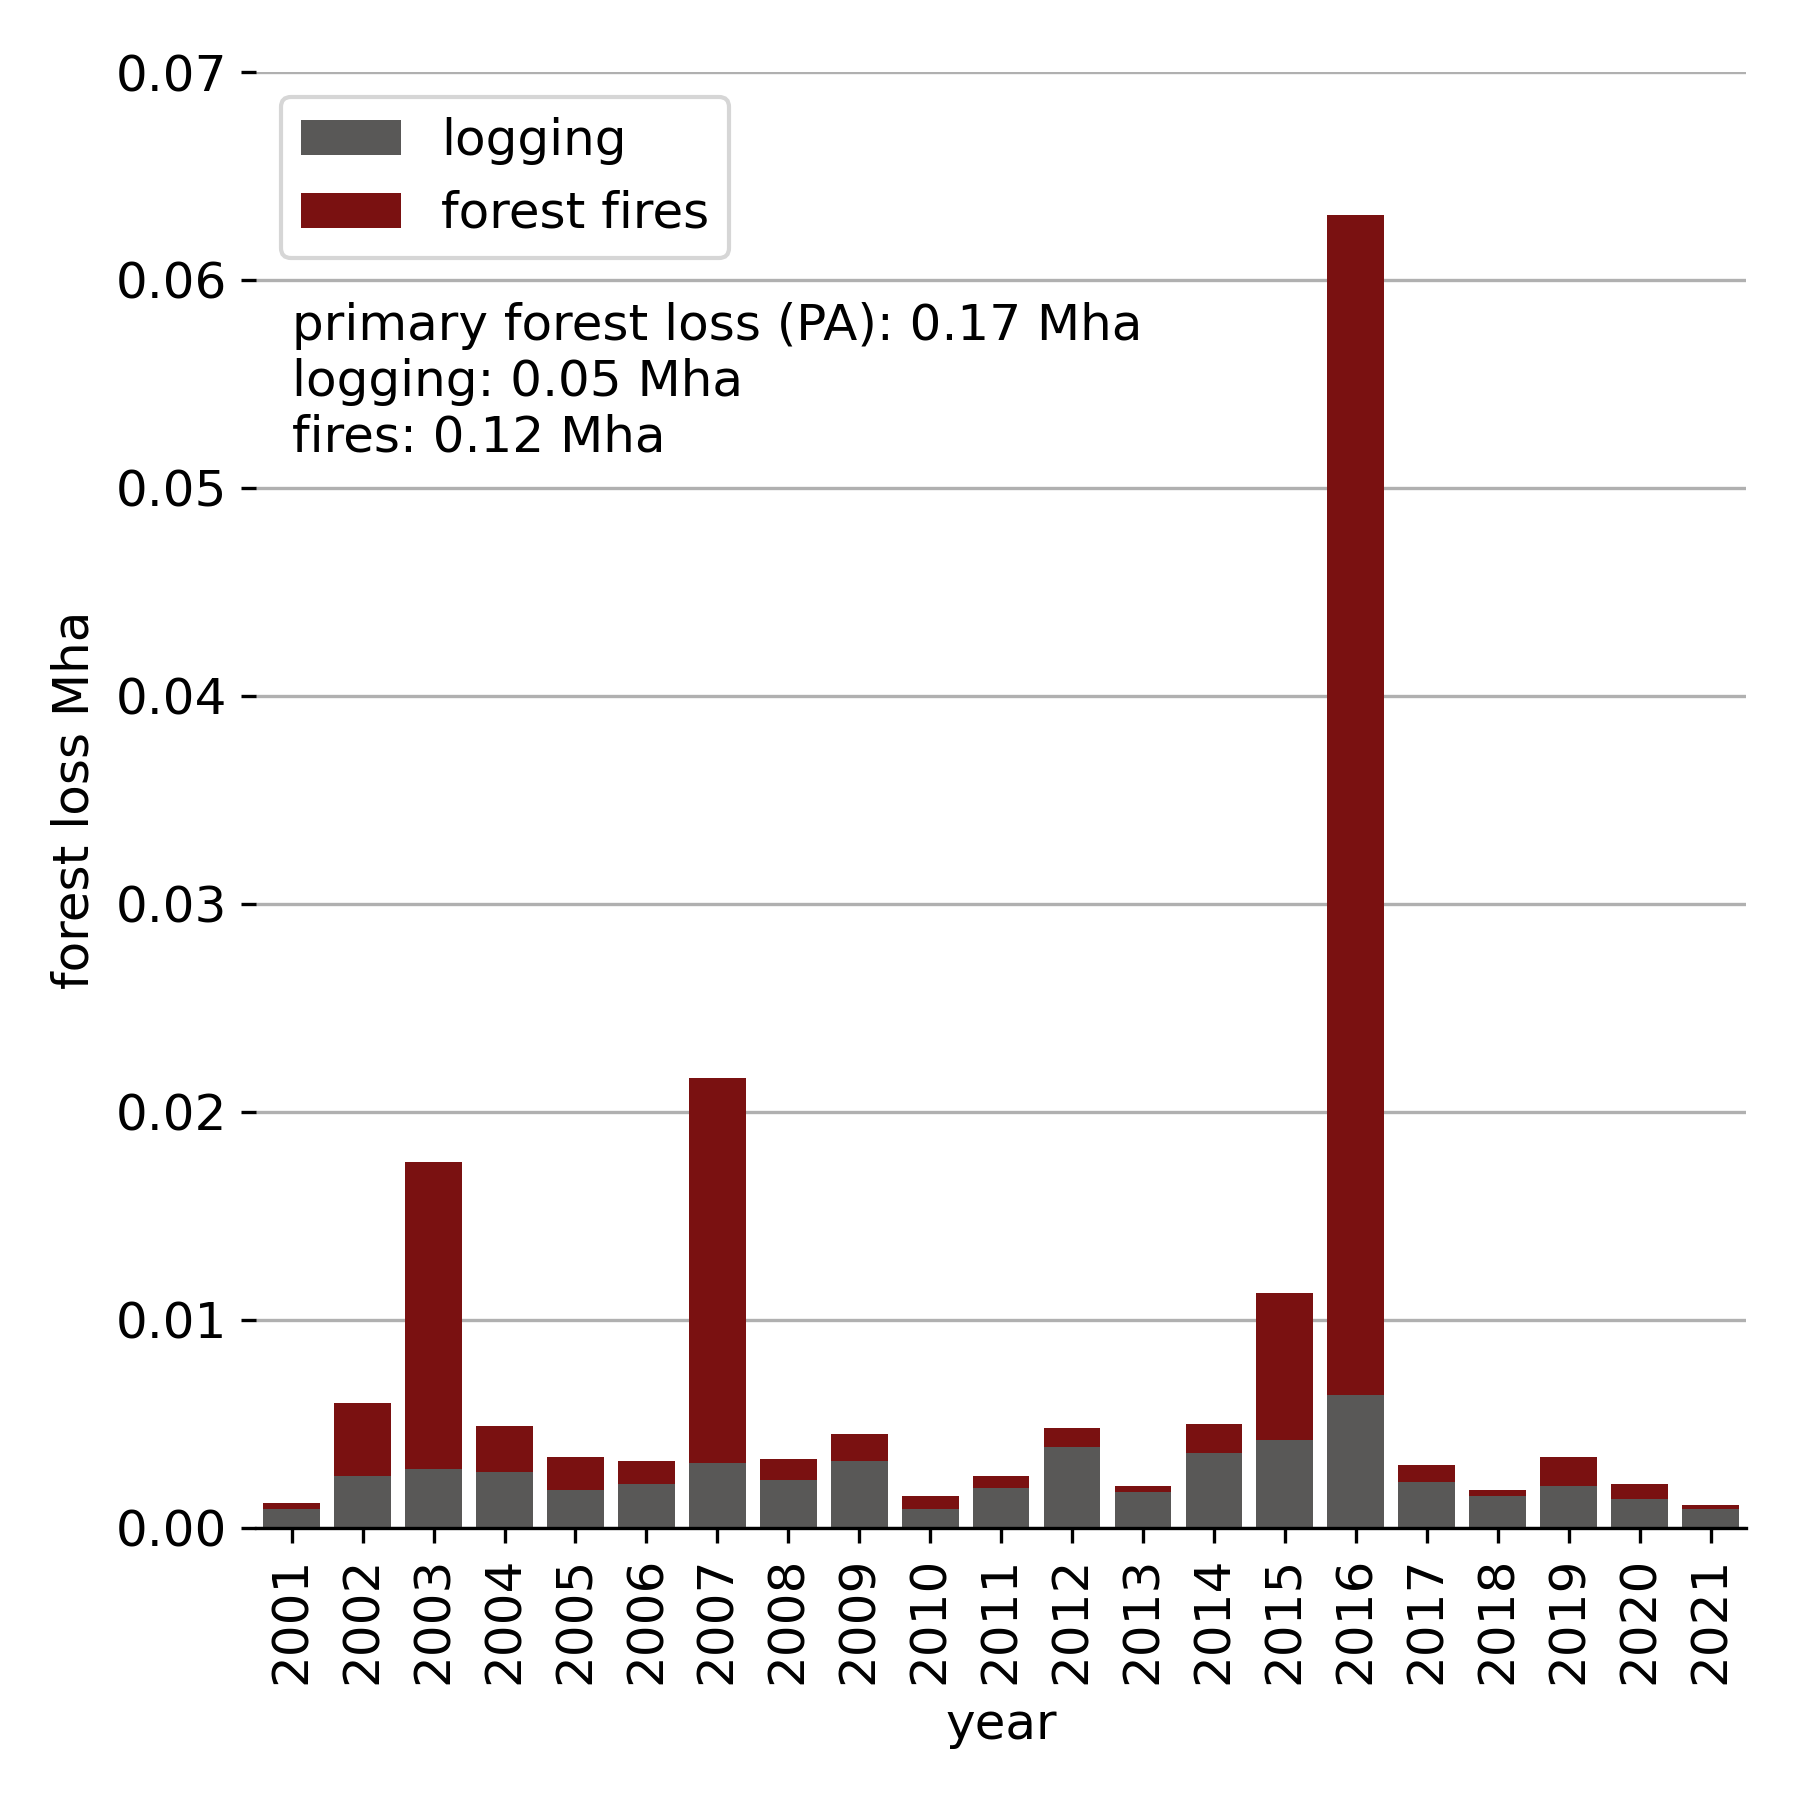
\includegraphics{text/../code/results/final_plots/deforestation_primary_forest_protected_areas.png}

}

}

\subcaption{\label{fig-bardeforestationprotectedprimary}Annual rates of
secondary forest loss within protected areas. The total area of primary
forest in these areas is 0.08 Mha.}
\end{minipage}%

\caption{\label{fig-forestlossbarcharts_PA}Deforestation within
protected areas, with the peak year in 2016.}

\end{figure}

\begin{figure}[H]

{\centering 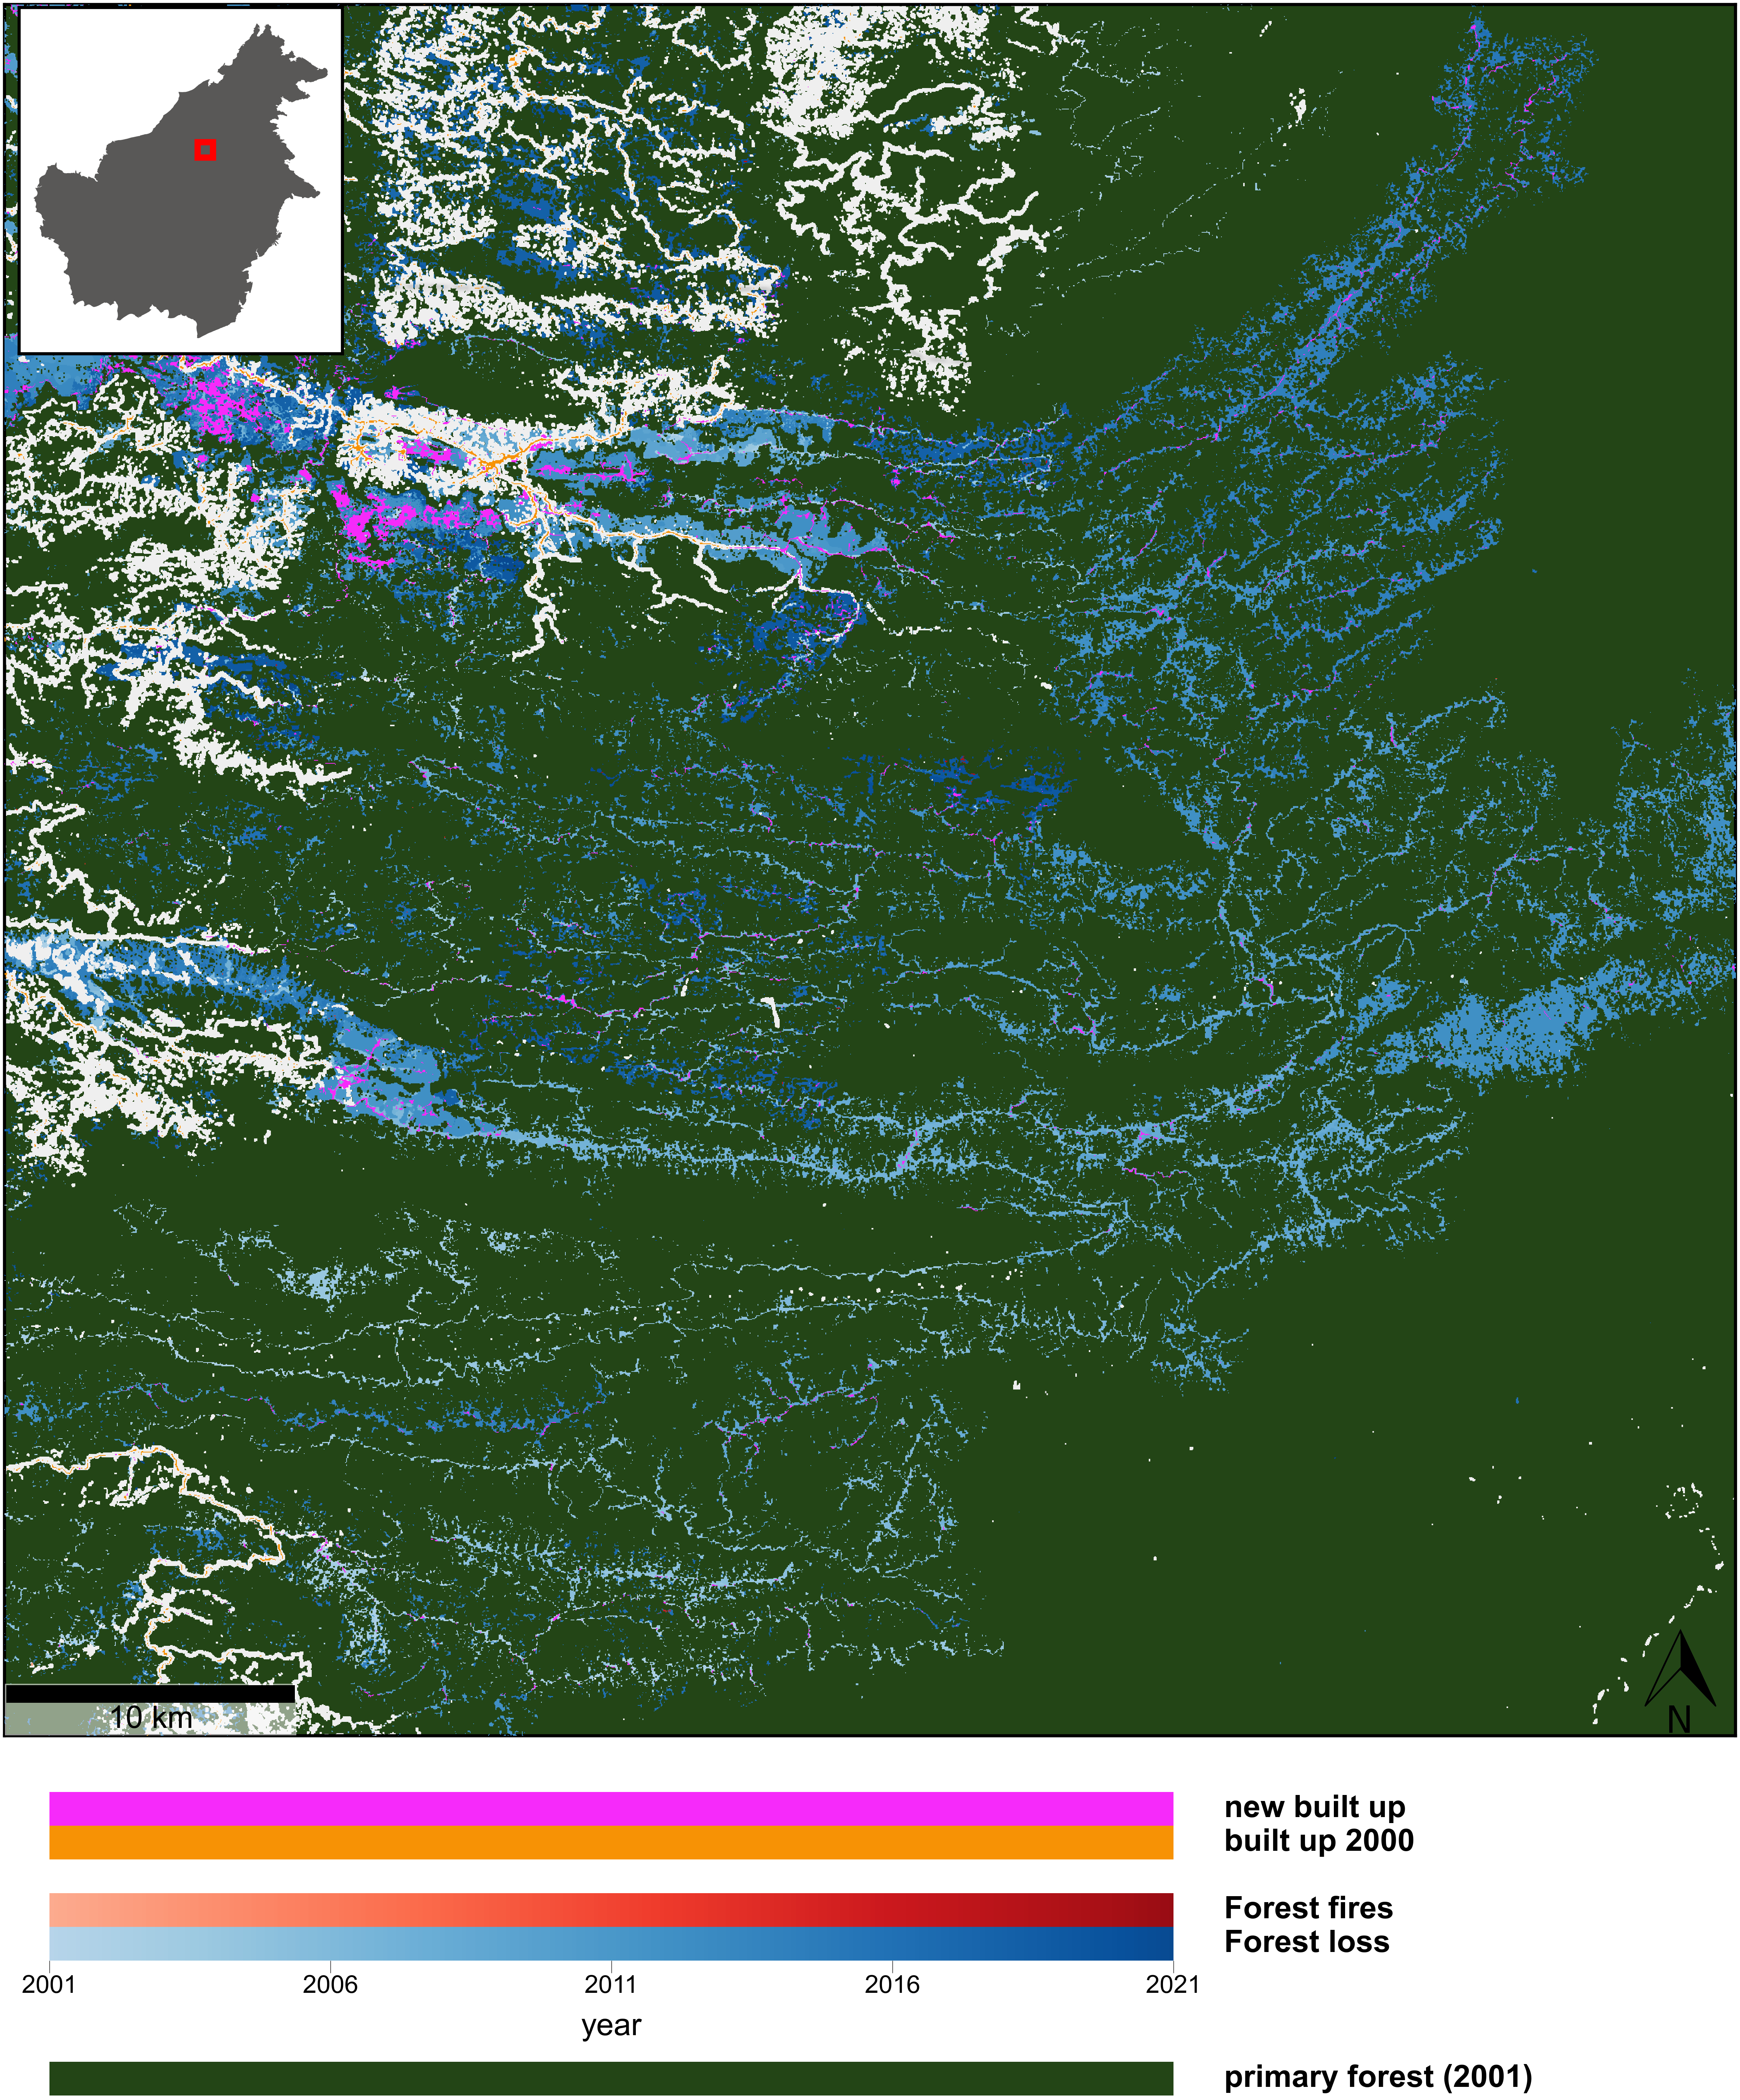
\includegraphics[width=0.95\textwidth,height=\textheight]{text/../code/results/maps/primary_deforestation.png}

}

\caption{\label{fig-map_deforestation_primary}Large areas in the
Malaysian part of Borneo where logging activities are penetrating deep
into the primary forest.}

\end{figure}

Protected areas cover 6.24 Mha, of which 0.08 Mha are secondary and 4.72
Mha is primary forest. Within protected areas, the main reason for
forest loss were fires, regardless of the classification as primary or
secondary forest. Forest fire and logging rates are similar
(Figure~\ref{fig-forestlossbarcharts_PA}). This is remarkable given that
secondary forests accounted for a massively smaller proportion of the
total area of PAs. Logging in protected areas occurred very limited with
an average of \textasciitilde2,500 ha per year being logged. However,
forest fires occurred irregularly, with a major spike in 2016 and other
substantial forest loss to fires in 2003, 2007, and 2015
(Figure~\ref{fig-bardeforestationprimary}). The majority of these large
forest fires were on the edges of the forest spanning large patches
(Figure~\ref{fig-mapforestfires}).

\newpage

\begin{figure}[H]

{\centering 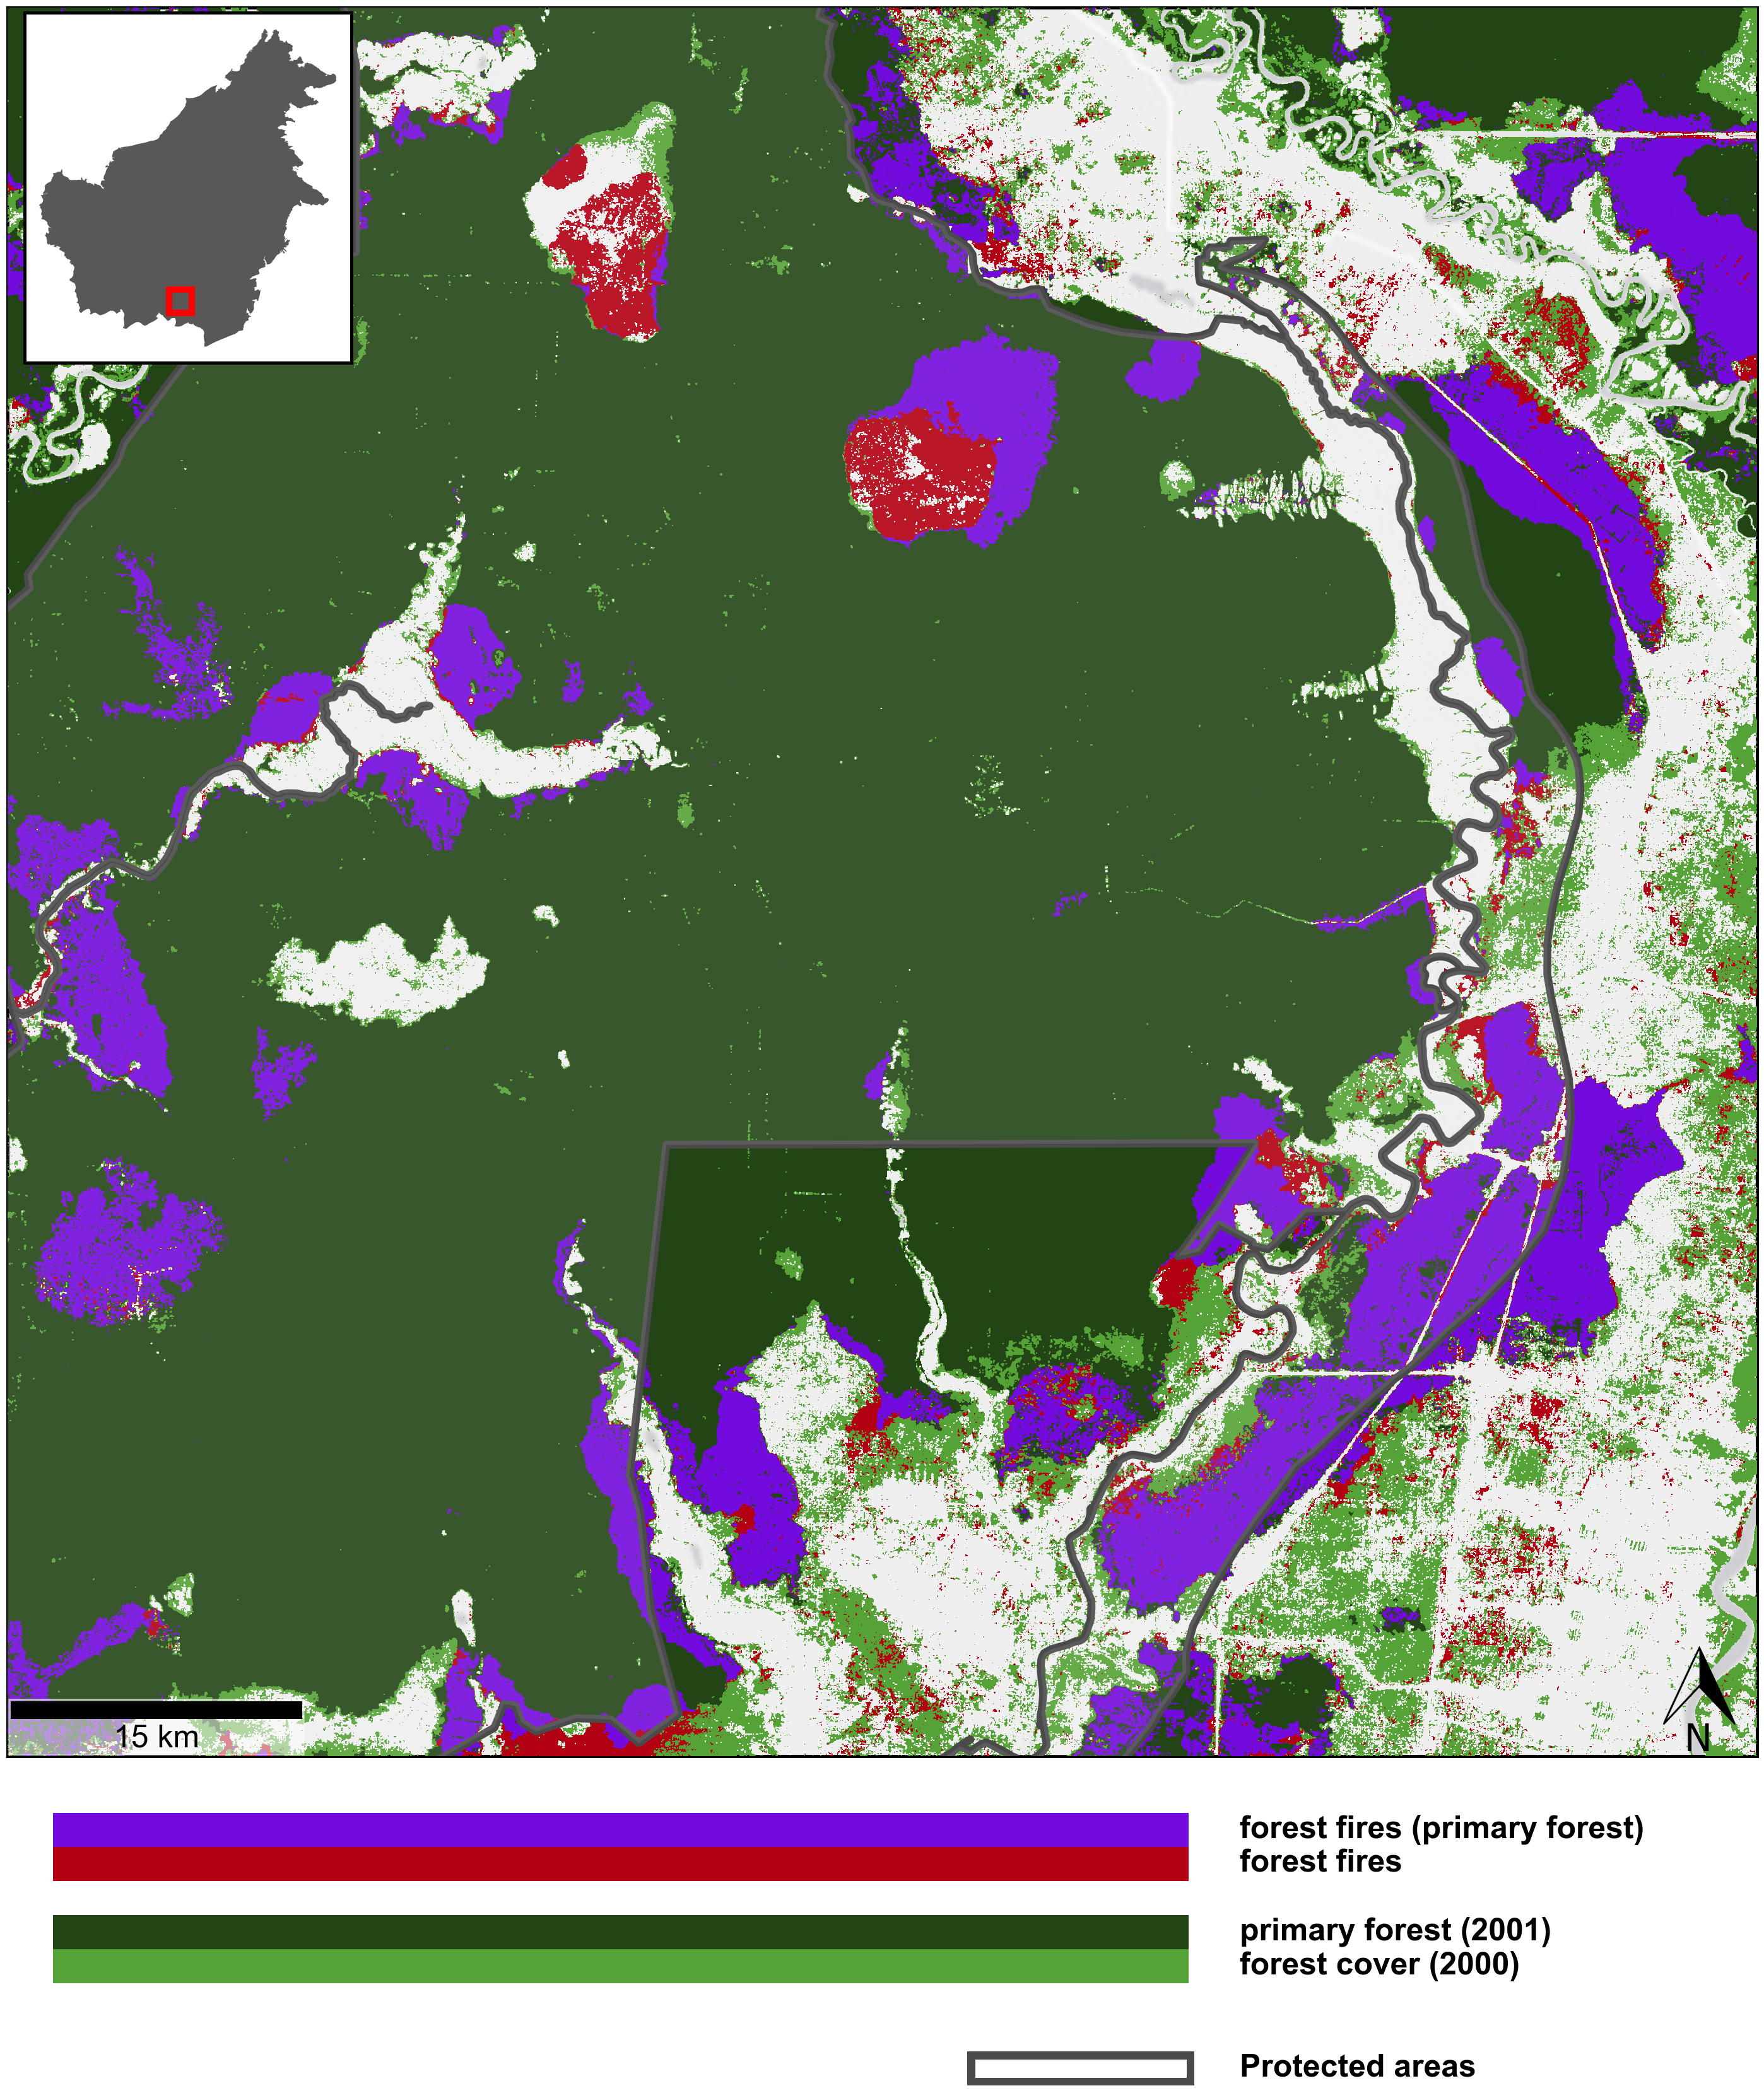
\includegraphics{text/../code/results/maps/deforestation_protected_areas_forest_fires.png}

}

\caption{\label{fig-mapforestfires}In this protected area it is clearly
visible, that forest fires (red) are the main drivers of deforestation
within protected areas. Large forest fires like these are the cause of
the outlier year 2016.}

\end{figure}

\hypertarget{oil-palm-1}{%
\section{Oil Palm}\label{oil-palm-1}}

Between 2001 and 2017 a total of 3.92 Mha new oil palm plantations were
detected. Comparable amounts were found on non-forested areas (1.46 Mha)
and secondary forests (1.74 Mha), however, only about half as much was
found on primary forests (0.71 Mha). While from 2001-2008
\textasciitilde0.15 Mha new plantations were recorded annualy, there was
almost twice as much in the following years with about 0.3 Mha per year.
After the maximum value of 0.45 Mha in 2015, the newly discovered
plantations decreased slightly in the most recent available years
(Figure~\ref{fig-bar_opoverview}). More than half (2.37 Mha) of the new
oil palm plantations occurred subsequently to deforestation
(Figure~\ref{fig-bar_opdeforestation}). Fires before new oil palm
plantations were discovered scarcely (0.07 Mha; Annex IX).

\begin{figure}

\begin{minipage}[t]{0.49\linewidth}

{\centering 

\raisebox{-\height}{

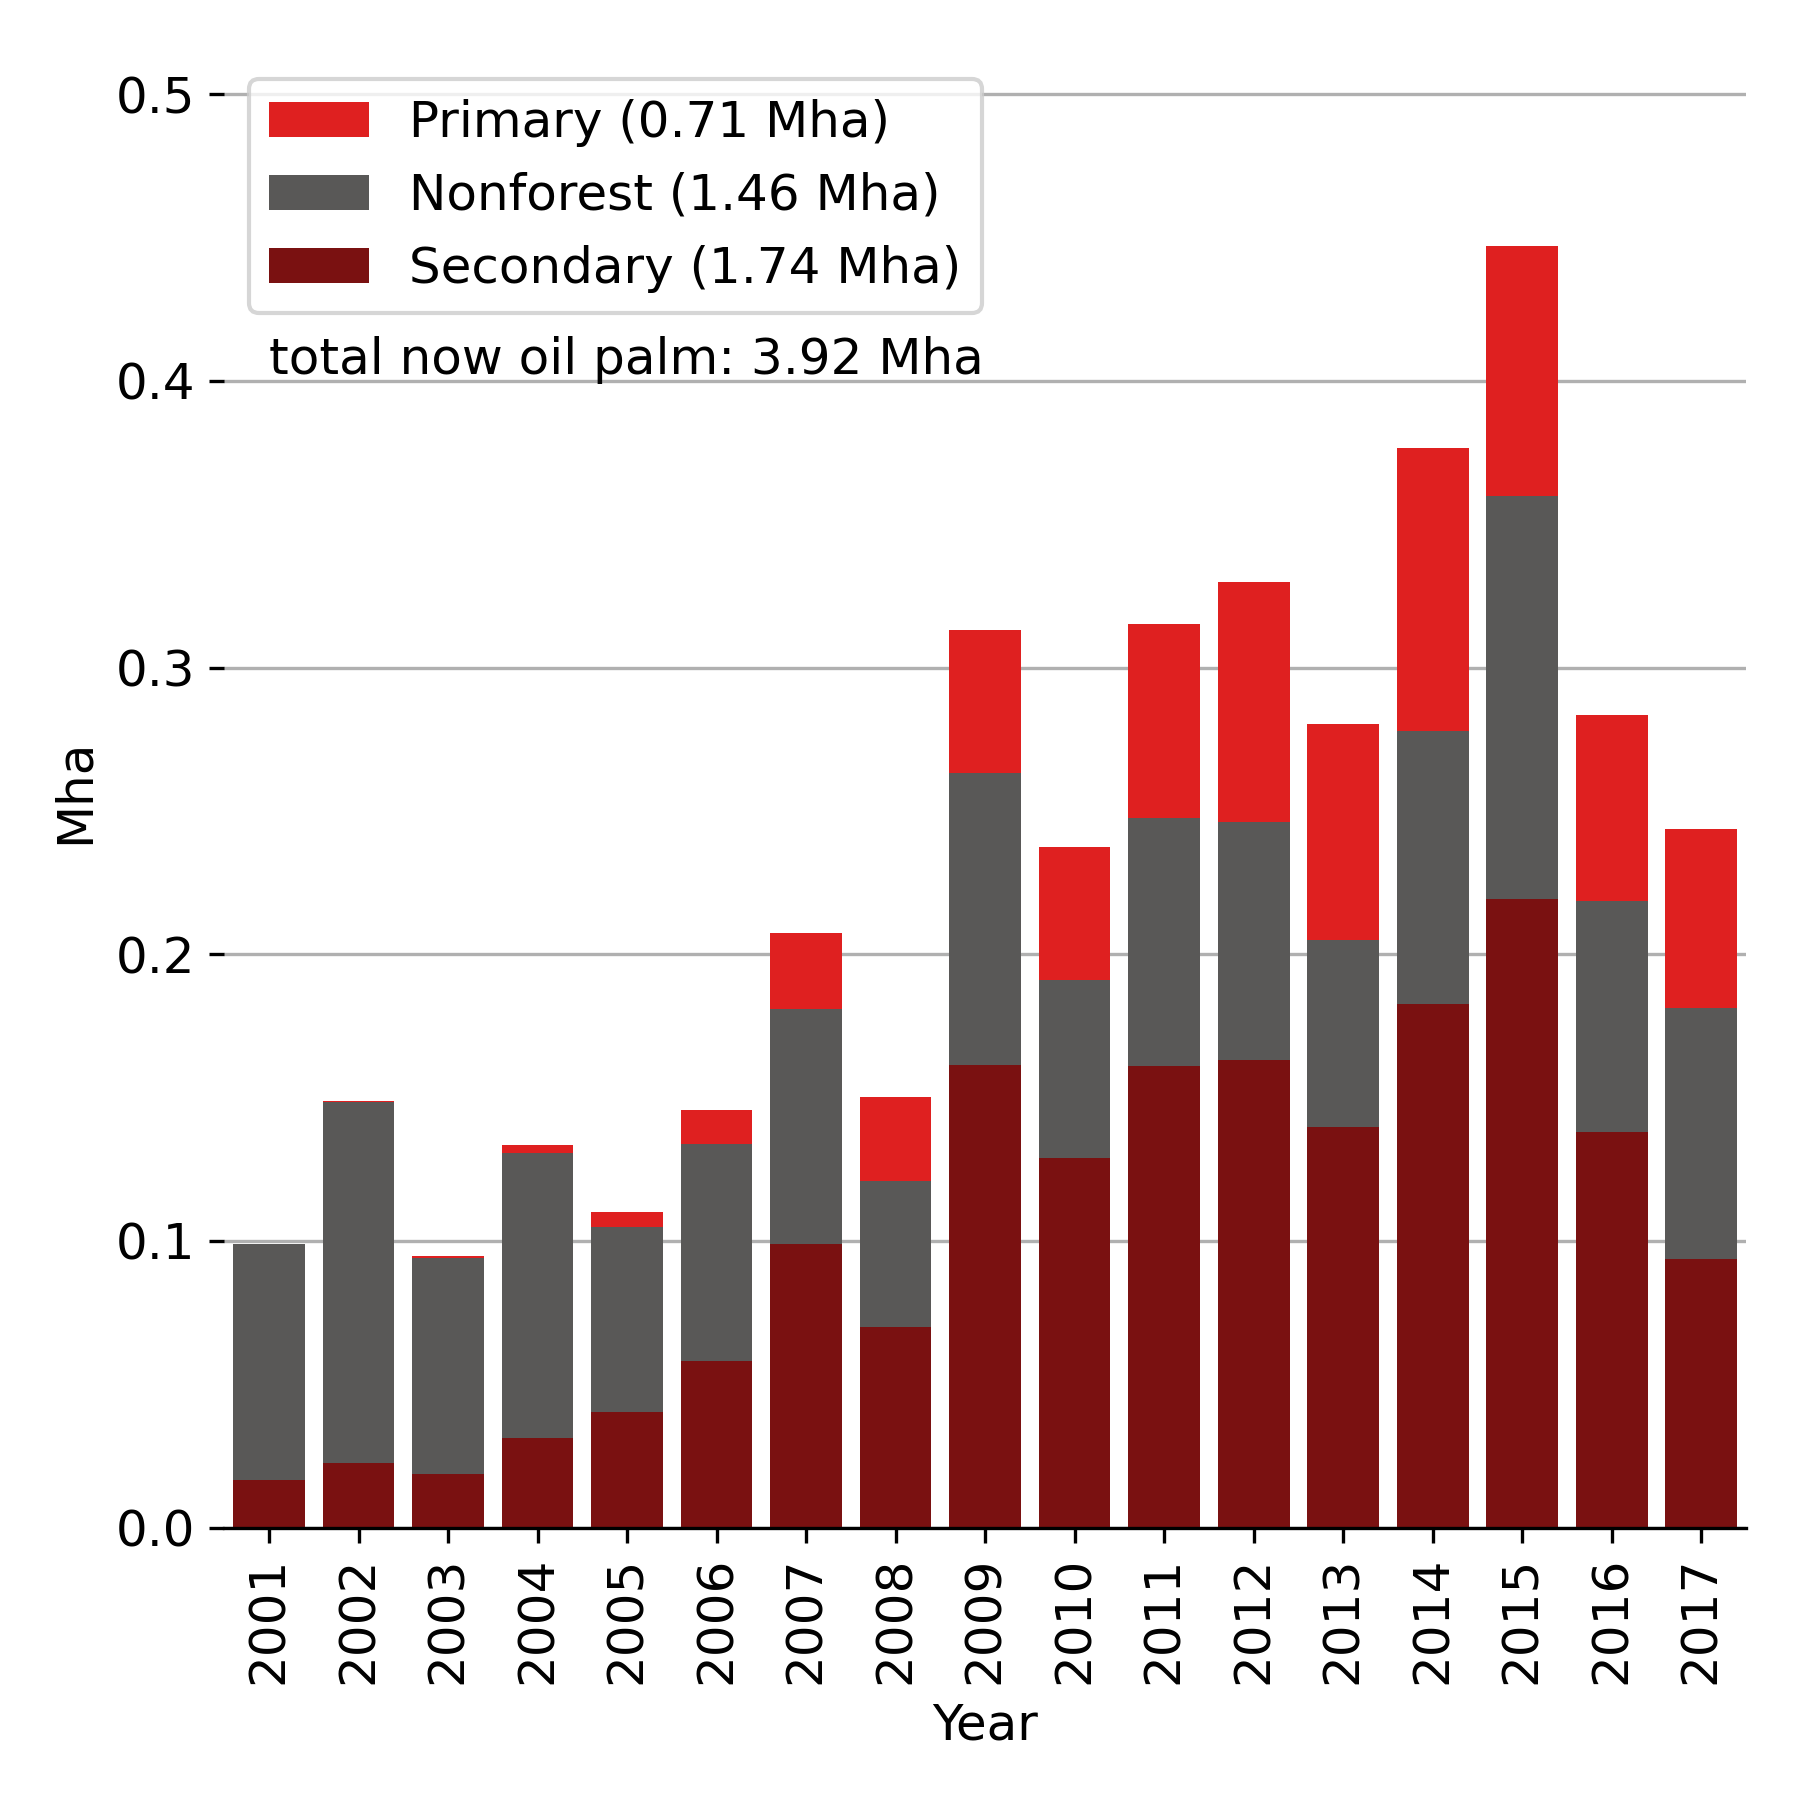
\includegraphics{text/../code/results/final_plots/oilpalm_overview.png}

}

}

\subcaption{\label{fig-bar_opoverview}Overview of where new oil palm
plantations were detected.}
\end{minipage}%
%
\begin{minipage}[t]{0.02\linewidth}

{\centering 

~

}

\end{minipage}%
%
\begin{minipage}[t]{0.49\linewidth}

{\centering 

\raisebox{-\height}{

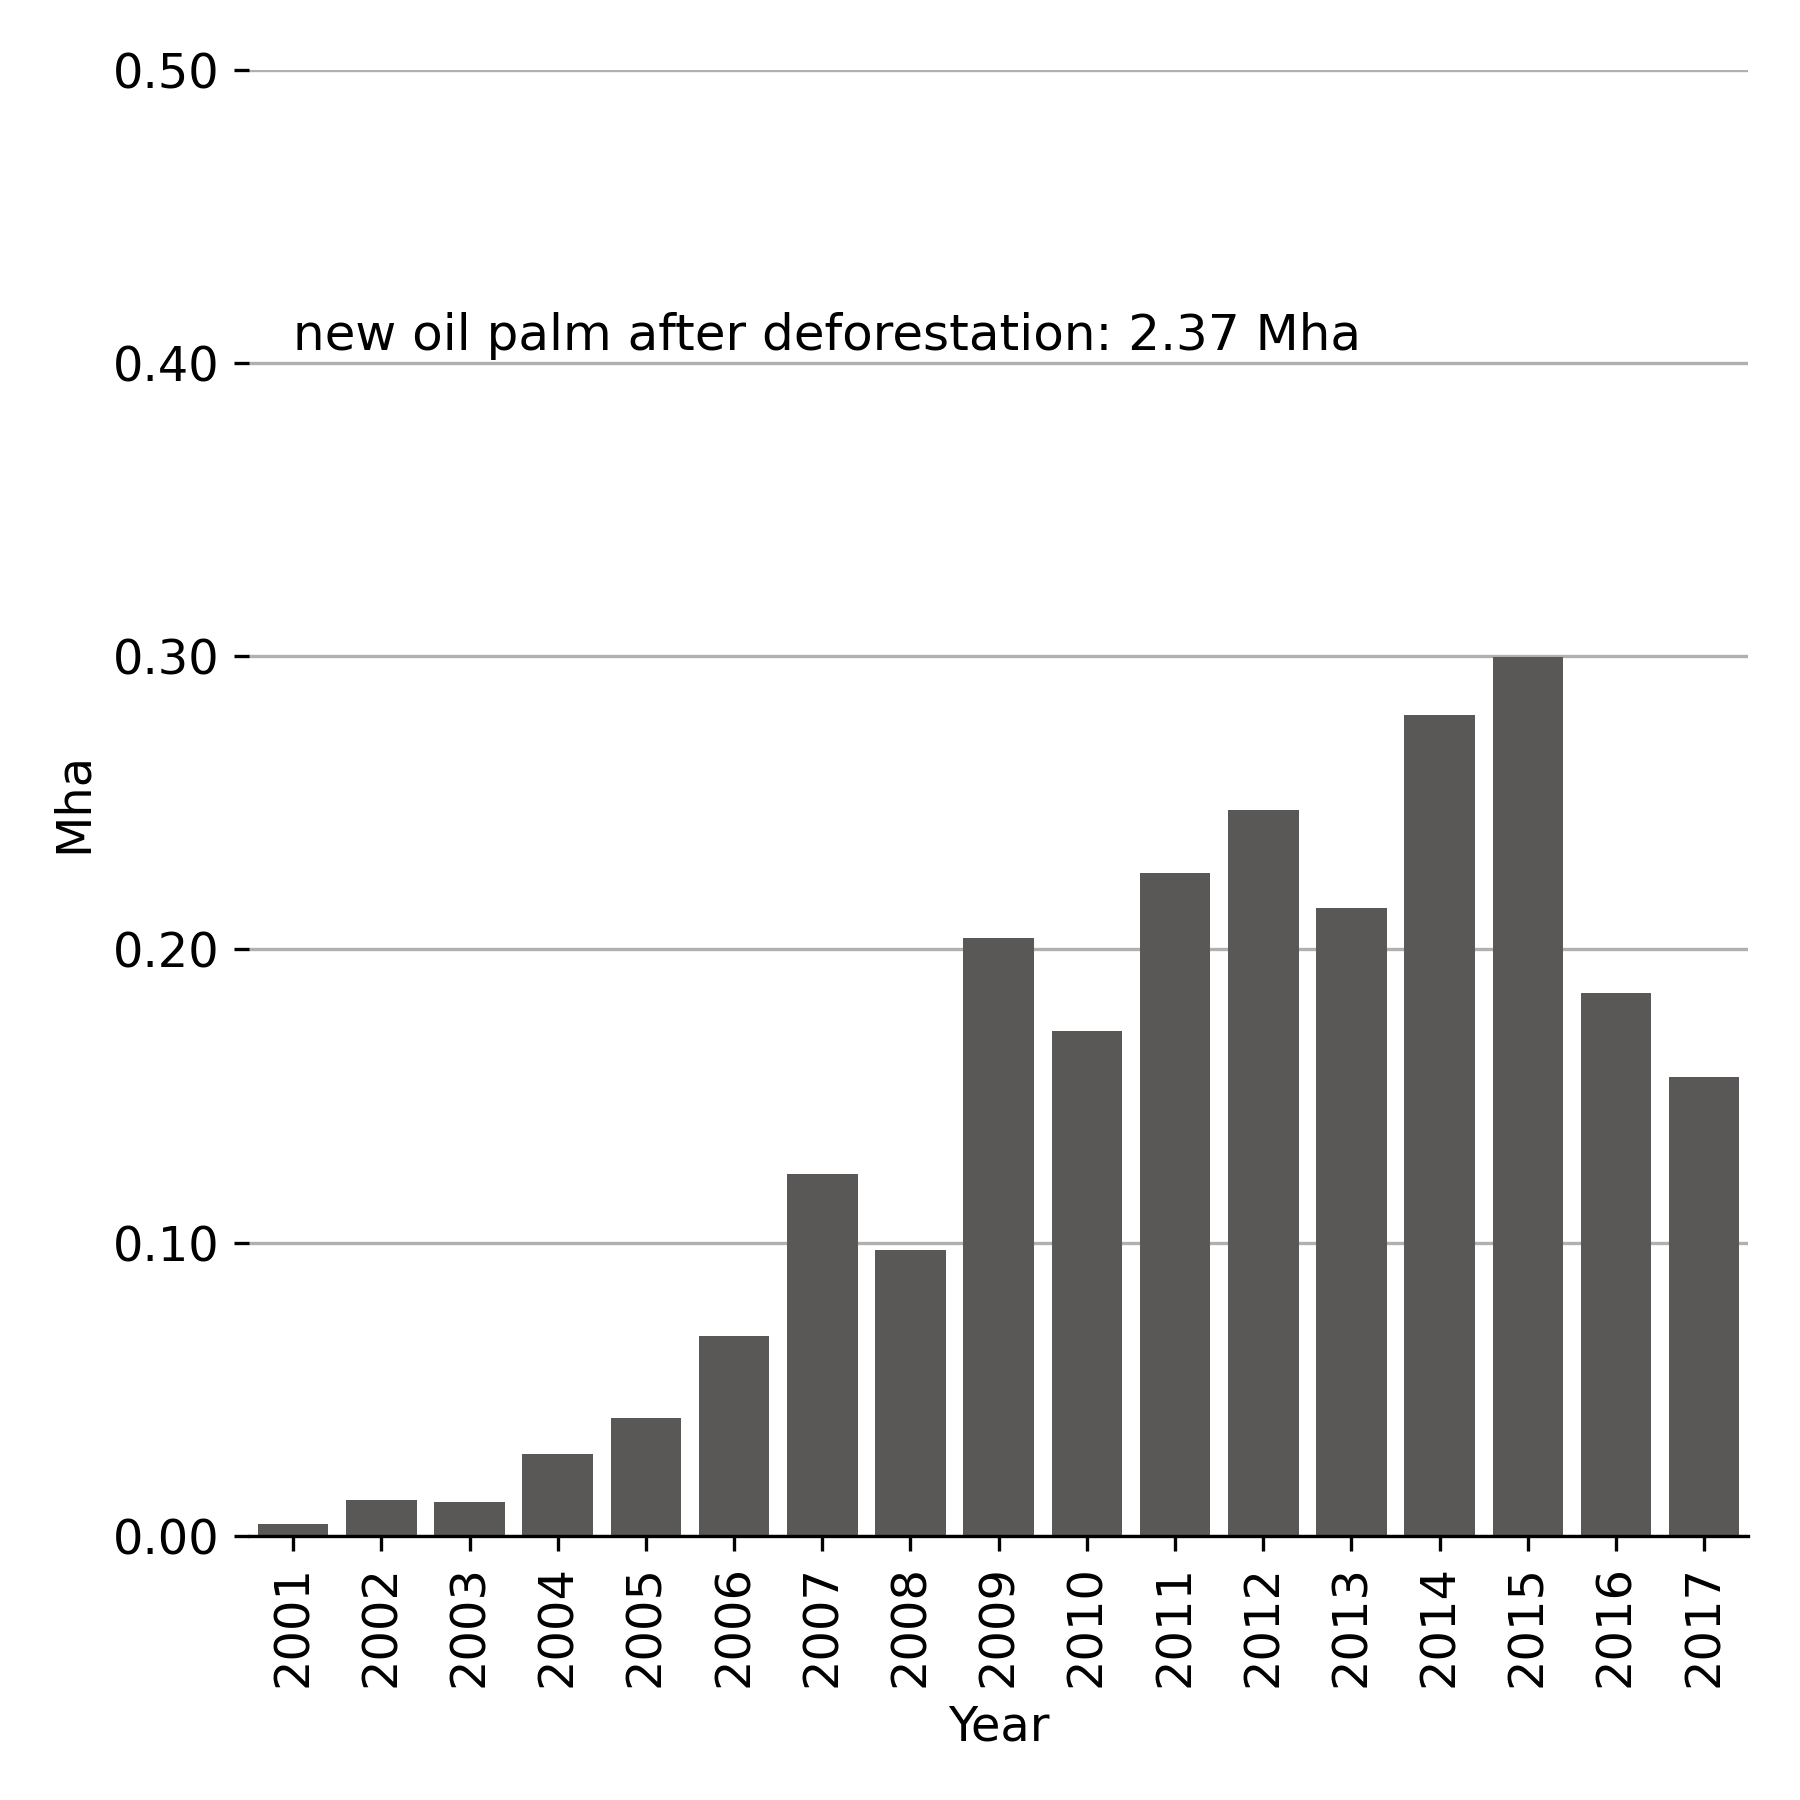
\includegraphics{text/../code/results/final_plots/new_oil_palm_after_deforestation.png}

}

}

\subcaption{\label{fig-bar_opdeforestation}Newly detected oil palm
plantations after deforestation.}
\end{minipage}%

\caption{\label{fig-barchart_op}New oil palm plantations where they
occur (\textbf{a}) and the portion which is found after deforestation
(\textbf{b}).}

\end{figure}

New industrial oil palm plantations are emerging in large areas where
they can be easily identified with their distinct rectangular patterns,
and to a lesser extent, small clusters are also evident. There are some
typical rectangular plantation areas classified as deforested (at least
4 years before the last oil palm survey year) where oil palm was not
recorded to the edge of these areas.
(Figure~\ref{fig-map_deforestation_op_fires}).

\begin{figure}

{\centering 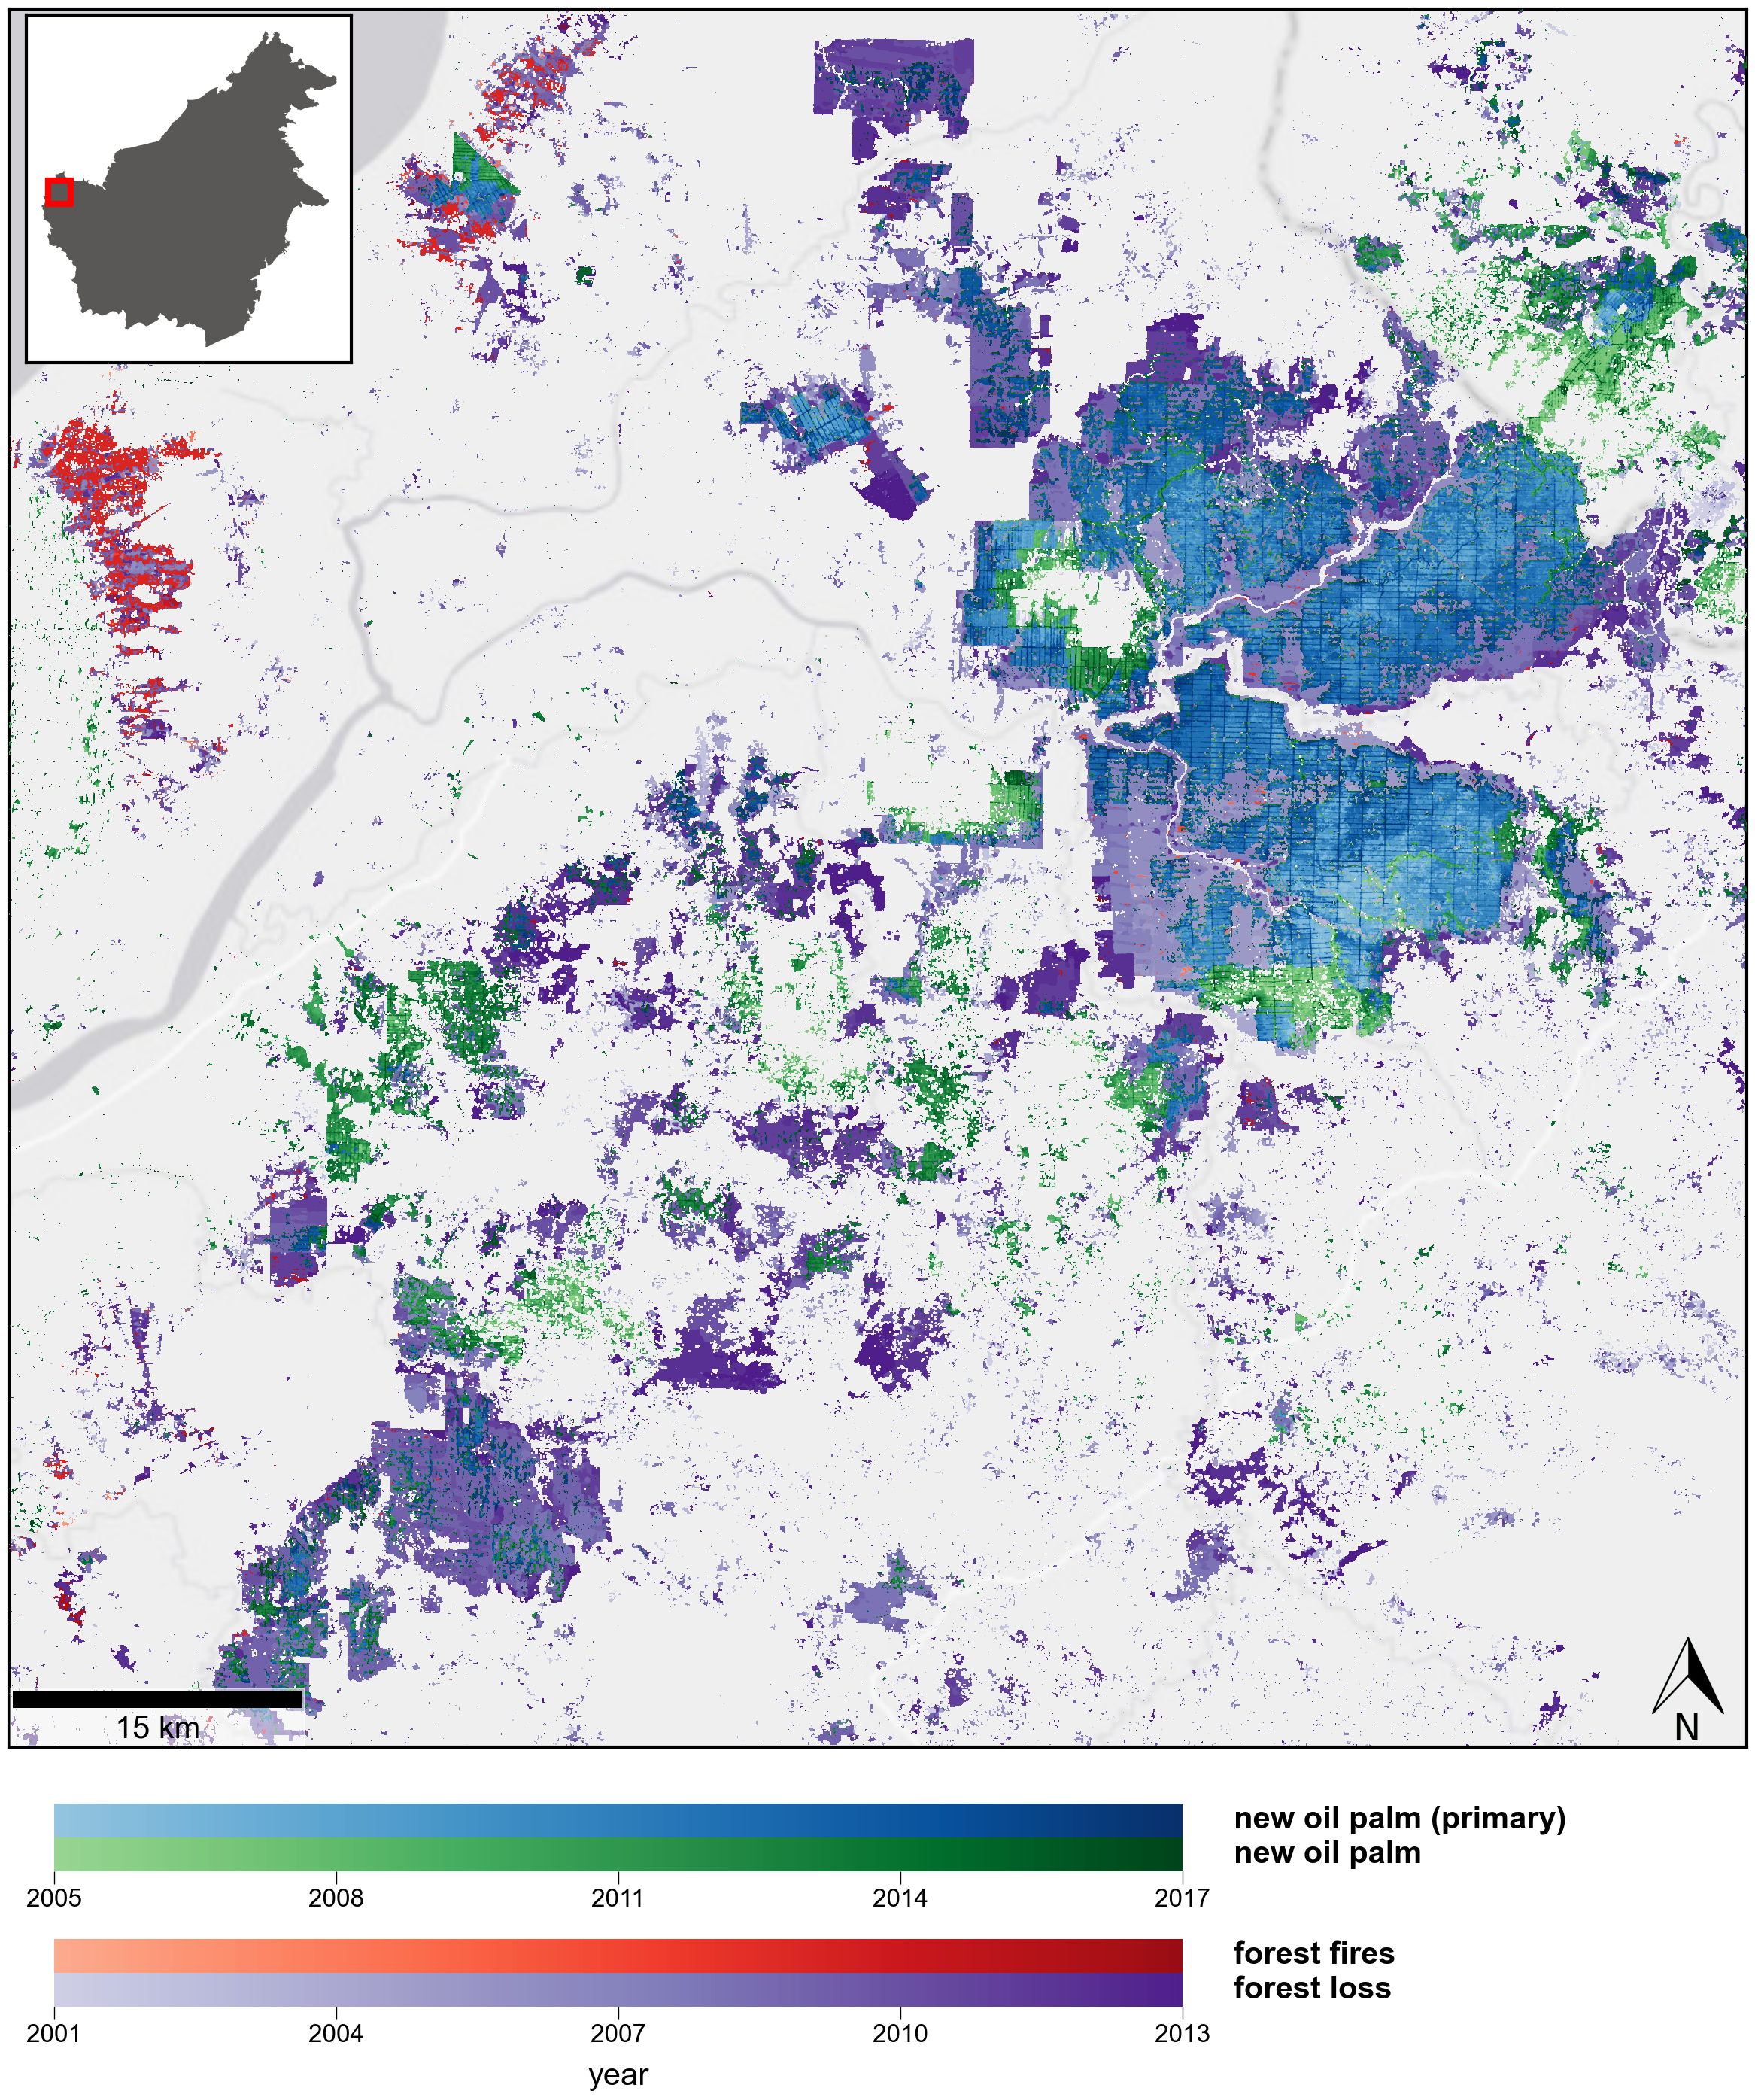
\includegraphics{text/../code/results/maps/deforestation_op_fires.png}

}

\caption{\label{fig-map_deforestation_op_fires}Large deforestation areas
are found on and nearby newly detected oil palm data. This extract also
shows one of the largest oil palm plantations on previous primary
forest. Some small-scale fires are visible in the southwest part of the
map.}

\end{figure}

\hypertarget{sec-resultsrspo}{%
\subsection{RSPO}\label{sec-resultsrspo}}

Except for the outlier years of 2015 and 2016, new oil palm discoveries
in uncertified RSPO concessions were similar, despite the smaller total
area of them. RSPO concessions accounted for 27.8\% (0.47 Mha) of all
Malaysian oil palm plantations (1.69 Mha), divided into 15.8\% certified
(0.27 Mha) and 12.0\% uncertified (0.19 million ha) concessions. A
noticeable difference is that 1.6\% of certified areas are located on
primary forest of 2001, compared to 6.4\% for the uncertified
concessions. The certifications were mainly issued in areas where palm
oil was already cultivated before the introduction of the RSPO label
(Figure~\ref{fig-RSPO_newop}).

\begin{figure}

\begin{minipage}[t]{0.49\linewidth}

{\centering 

\raisebox{-\height}{

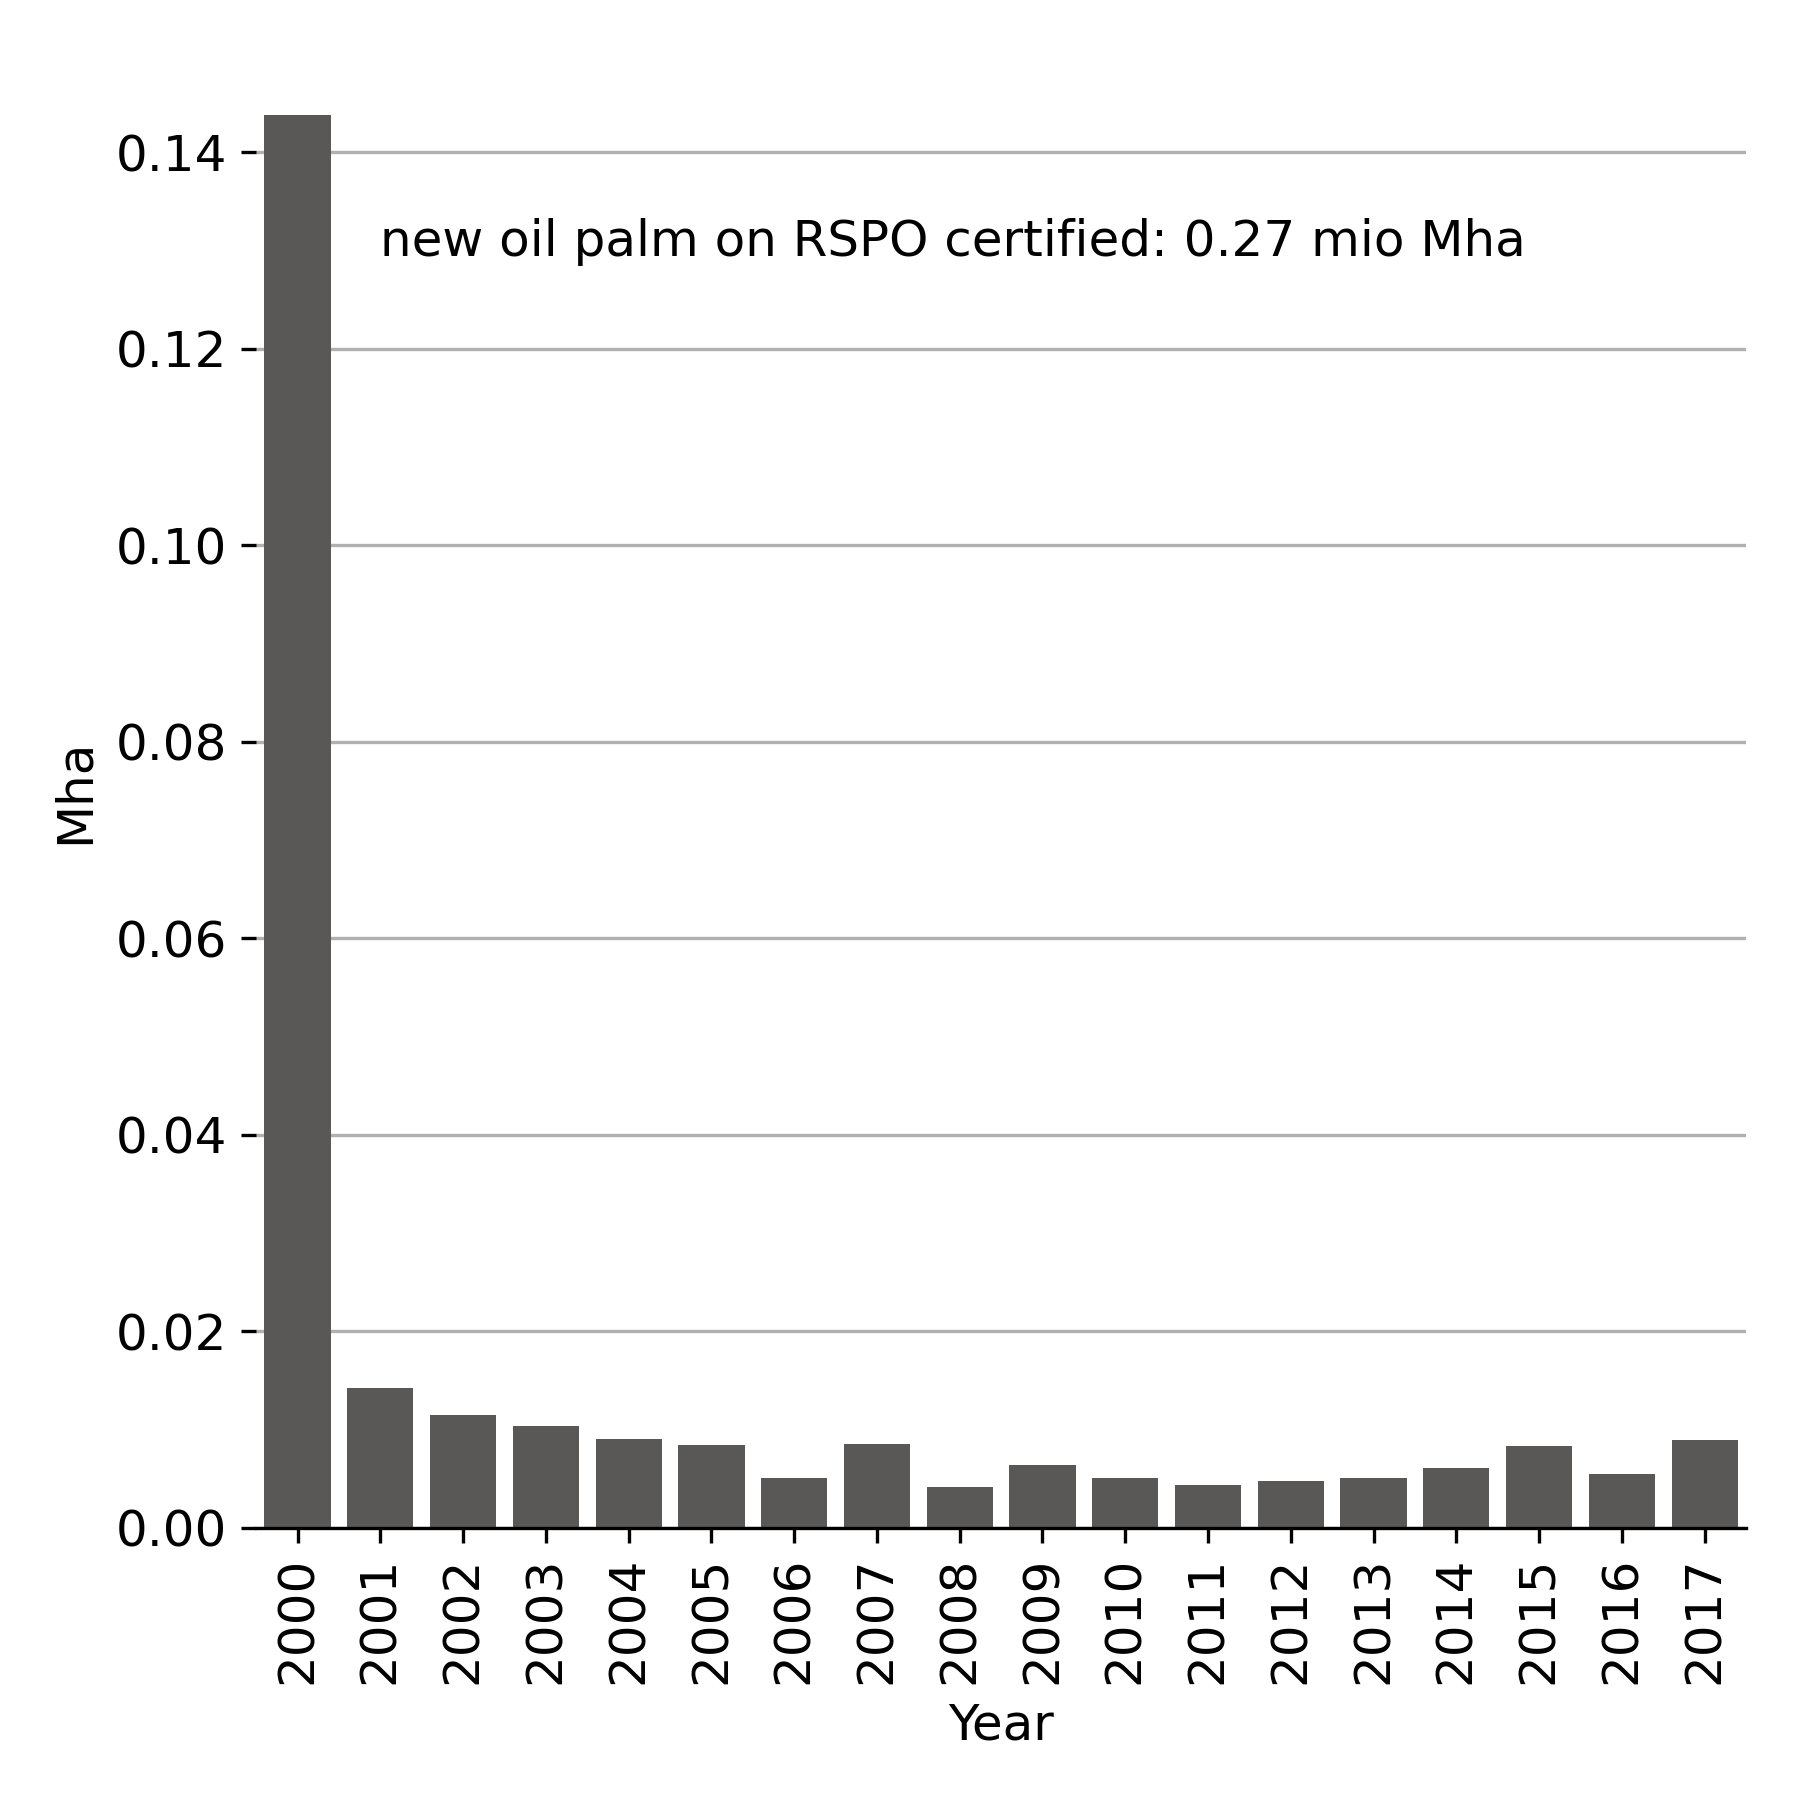
\includegraphics{text/../code/results/final_plots/oil_palm_in_RSPO_certified_regions.png}

}

}

\subcaption{\label{fig-RSPO_opcert}Amount of newly detected oil palm
plantations within RSPO certified concessions. Most of the oil palm
plantations already existed in the year 2000.}
\end{minipage}%
%
\begin{minipage}[t]{0.02\linewidth}

{\centering 

~

}

\end{minipage}%
%
\begin{minipage}[t]{0.49\linewidth}

{\centering 

\raisebox{-\height}{

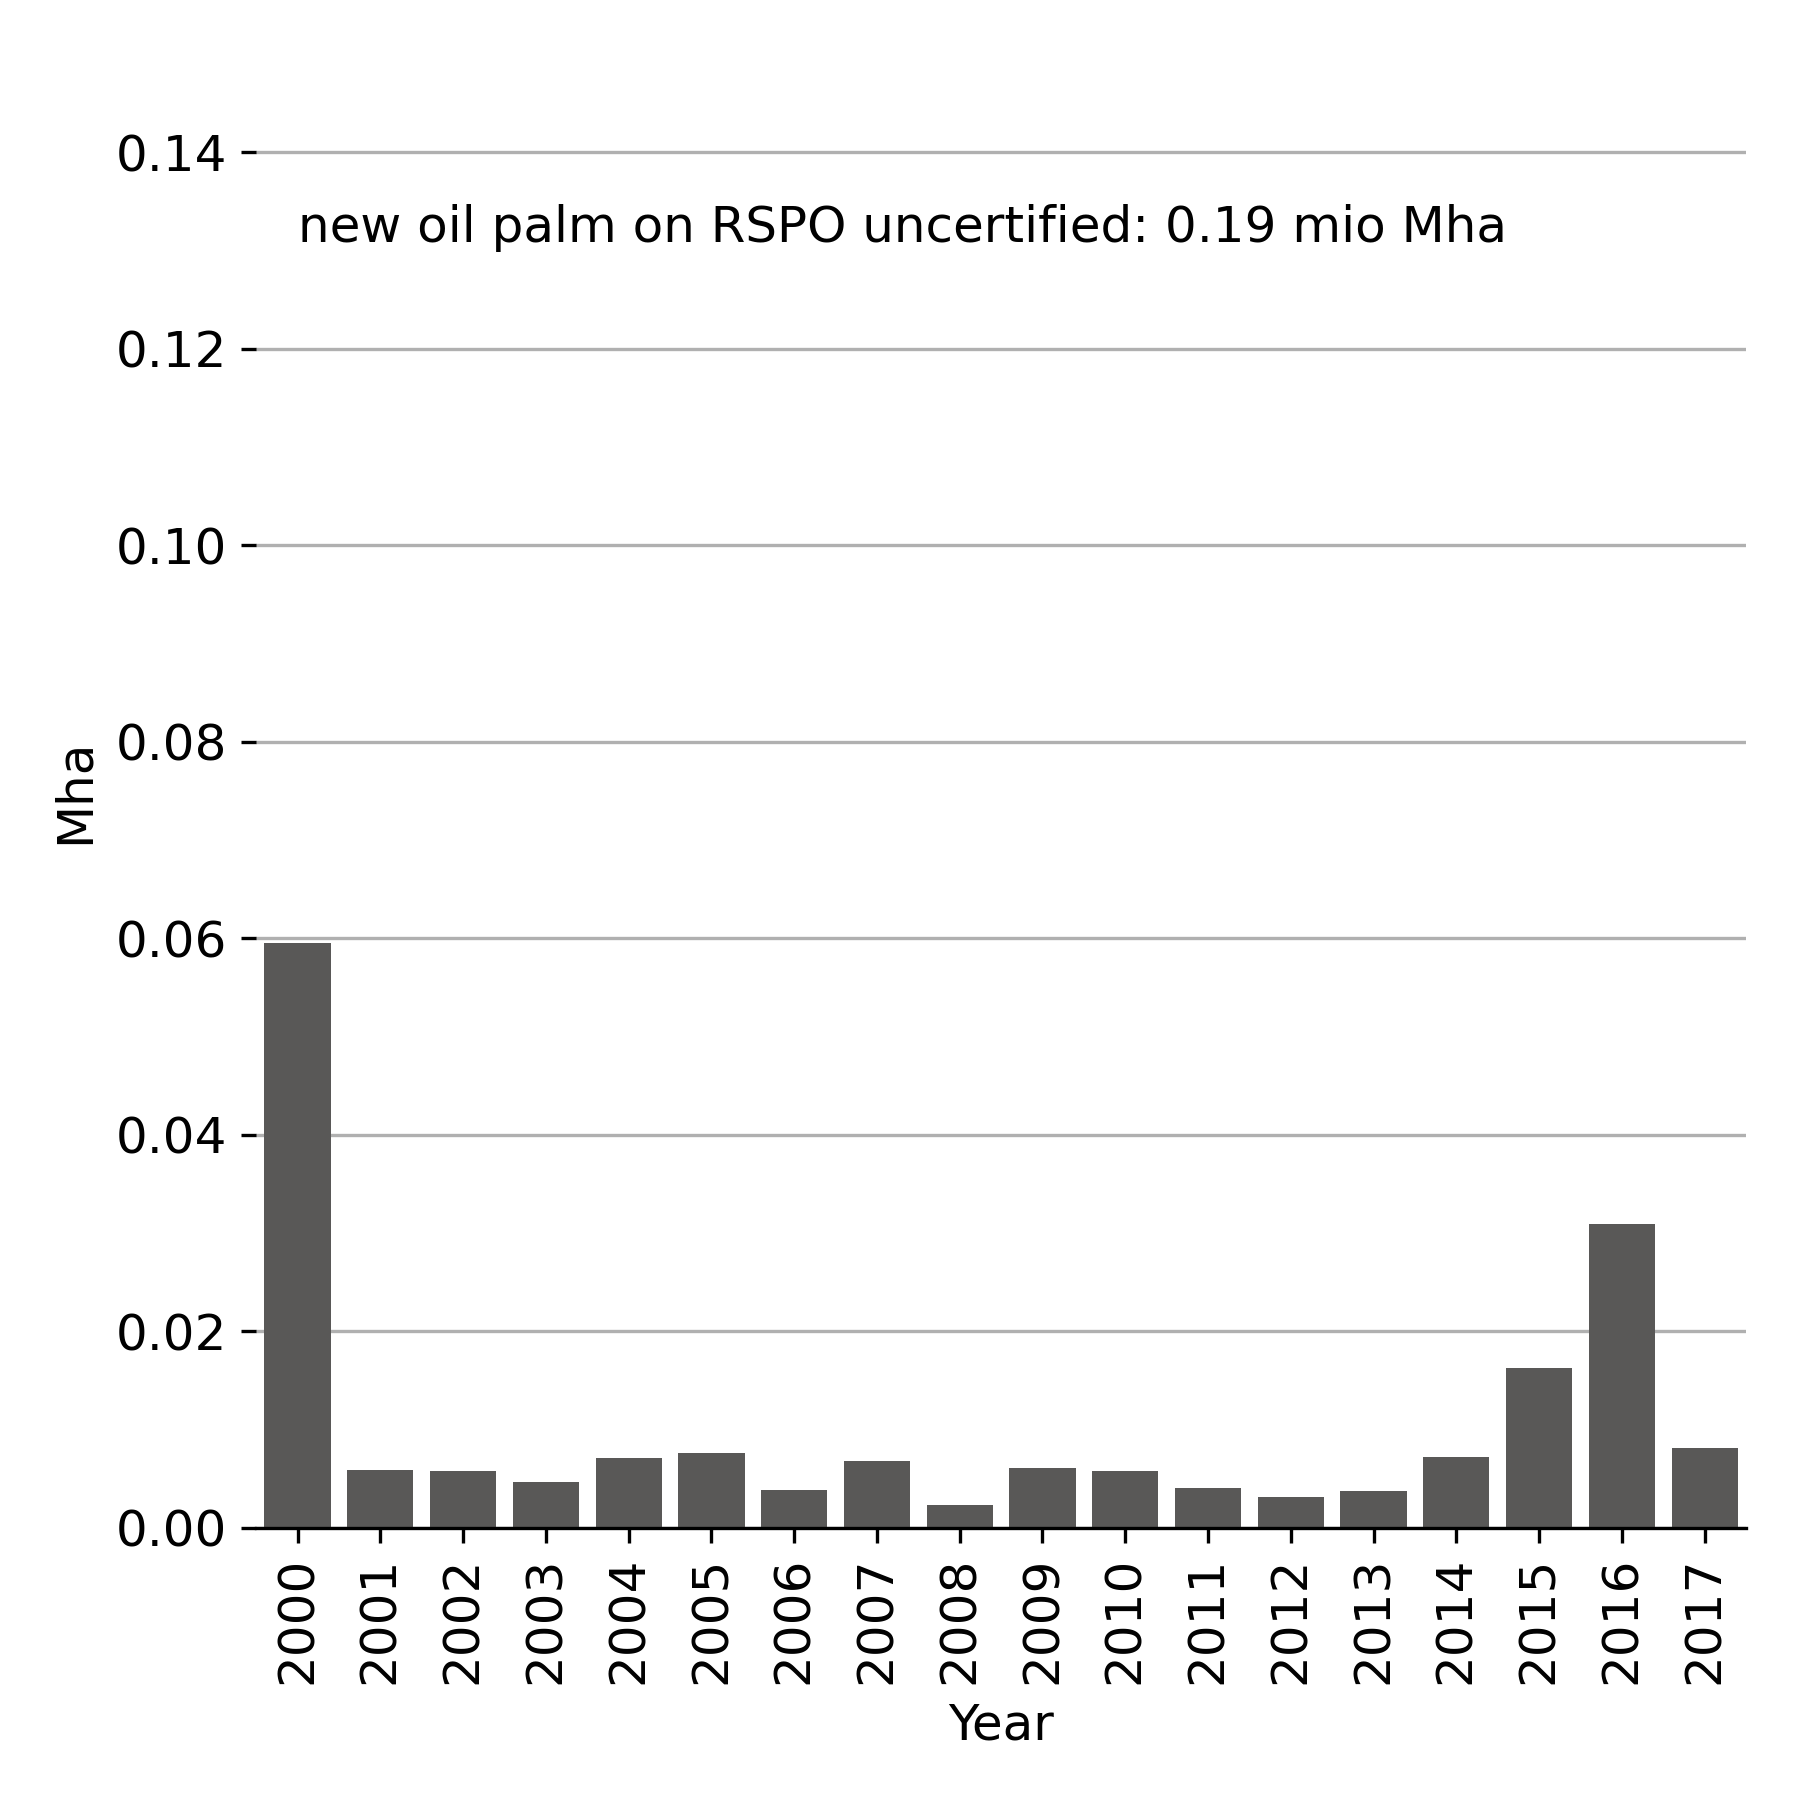
\includegraphics{text/../code/results/final_plots/oil_palm_in_RSPO_uncertified_regions.png}

}

}

\subcaption{\label{fig-RSPO_opnocert}Amount of newly detected oil palm
plantations within RSPO uncertified concessions. Besides the majority
being already used as oil palm plantations.}
\end{minipage}%

\caption{\label{fig-RSPO_newop}Newly discovered oil palm in (\textbf{a})
certified and (\textbf{b}) uncertified RSPO concessions (status 2023).}

\end{figure}

The highest primary forest loss rates within RSPO certified concessions
occured in the years 2002 (1000 ha) and 2004 (1080 ha). While around 200
hectares of primary forest were still being cut down each year until
2010, rates have sharply dropped to almost zero
(Figure~\ref{fig-RSPO_primaryloss}). In uncertified concessions,
two-thirds of primary forest area was lost, with the peak years being
2009 (2570 ha) and 2012 (4125 ha; Figure~\ref{fig-RSPO_secondaryloss}).
Whereas secondary forest loss showed elevated deforestation rates from
2012 onwards in certified concessions compared with the previous decade,
the rates in the uncertified concessions were at a continuous level (see
annex VII).

\begin{figure}[H]

\begin{minipage}[t]{0.49\linewidth}

{\centering 

\raisebox{-\height}{

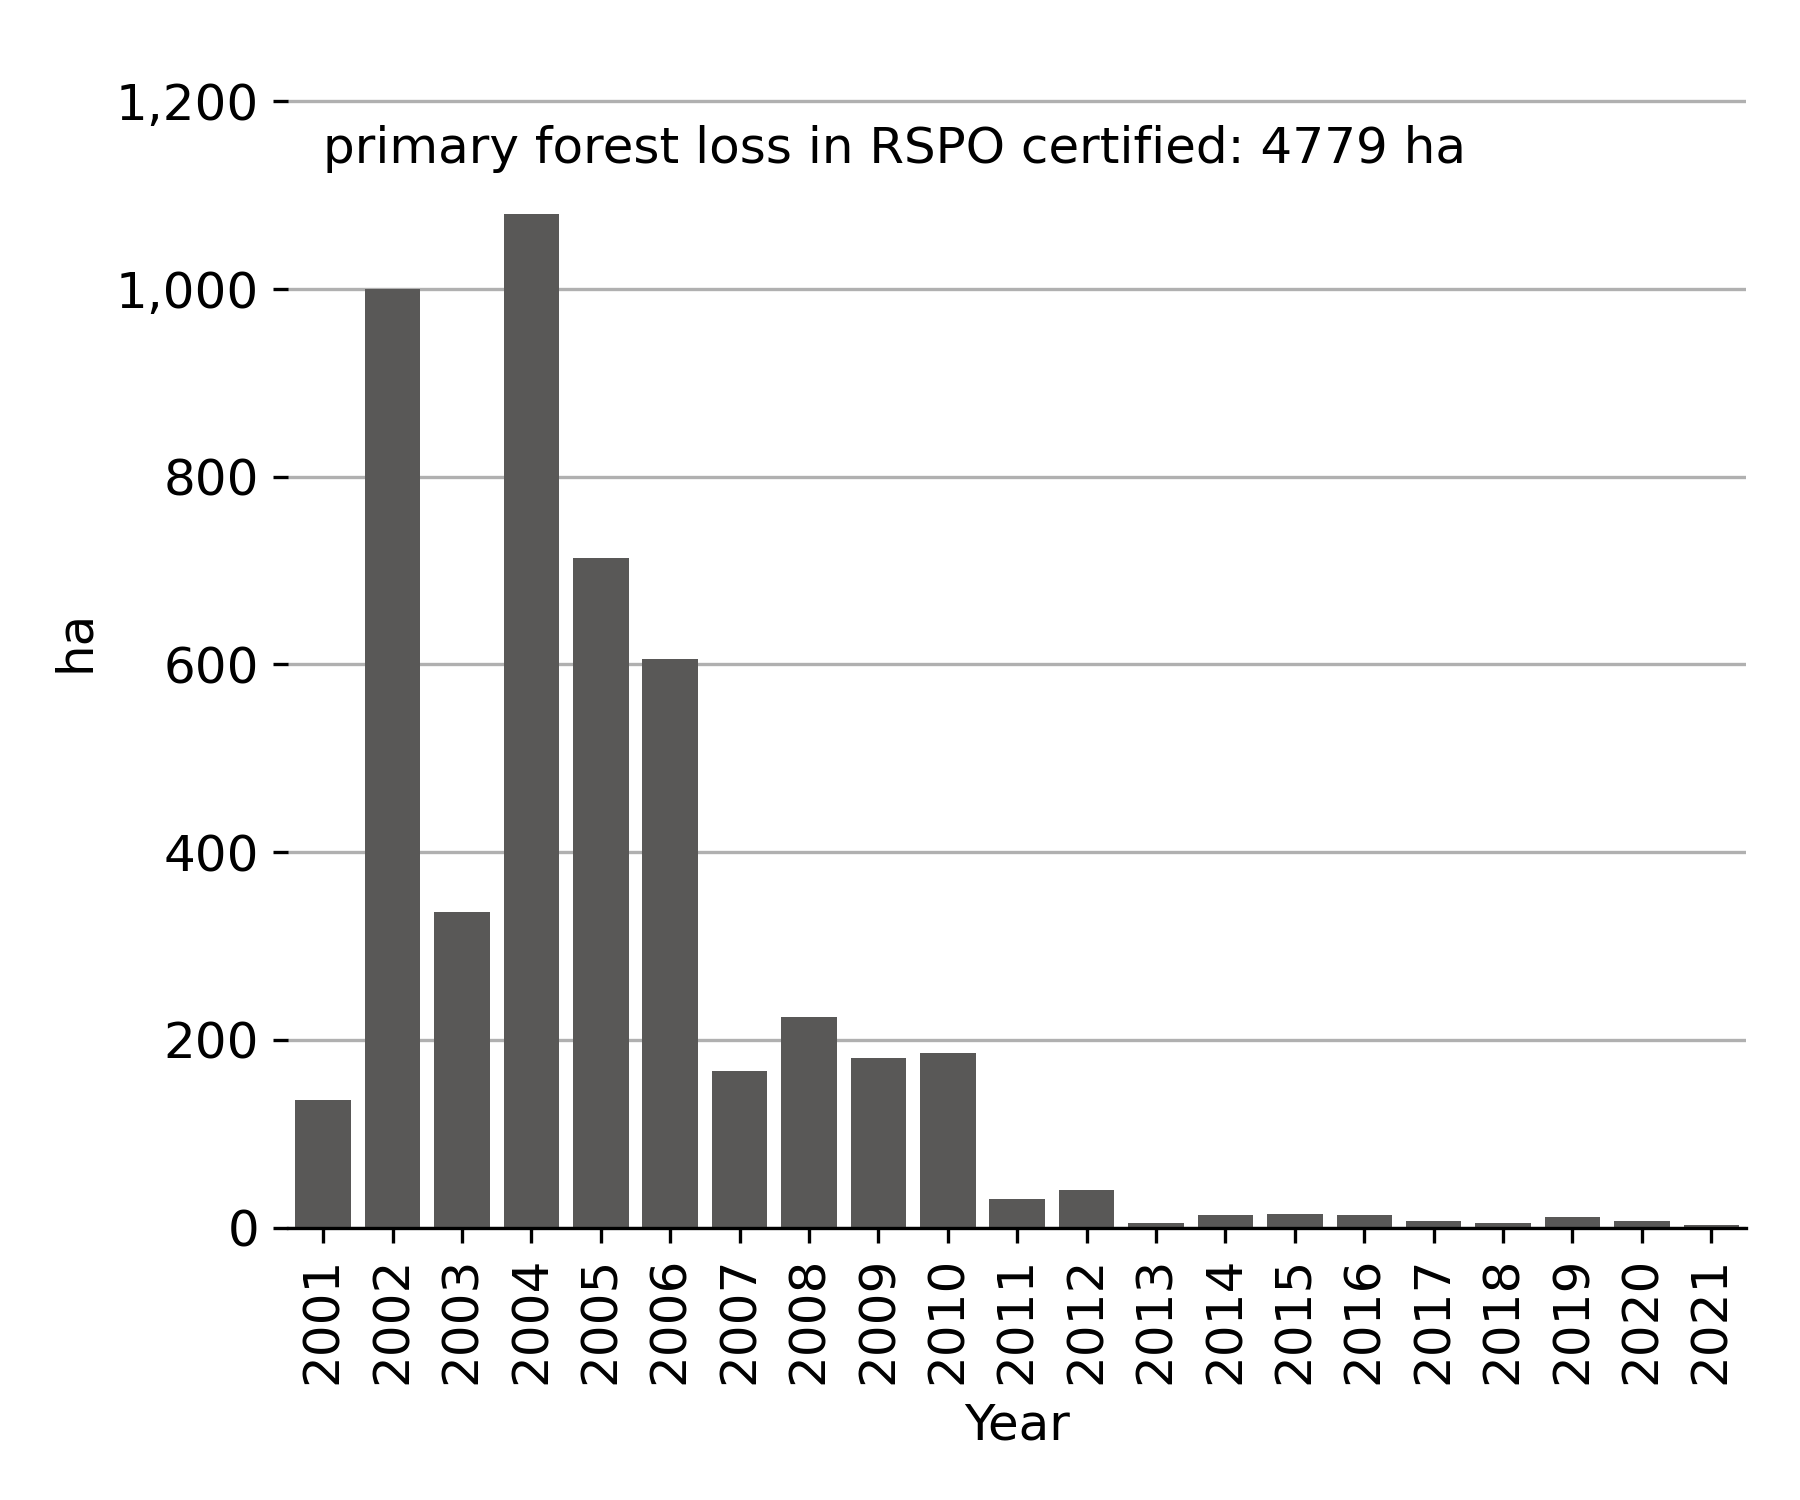
\includegraphics{text/../code/results/final_plots/RSPO_certified_primary_loss.png}

}

}

\subcaption{\label{fig-RSPO_primaryloss}Rates of primary forest loss
within certified RSPO concessions, with most forest loss occurring
before 2007 and halting from 2011.}
\end{minipage}%
%
\begin{minipage}[t]{0.02\linewidth}

{\centering 

~

}

\end{minipage}%
%
\begin{minipage}[t]{0.49\linewidth}

{\centering 

\raisebox{-\height}{

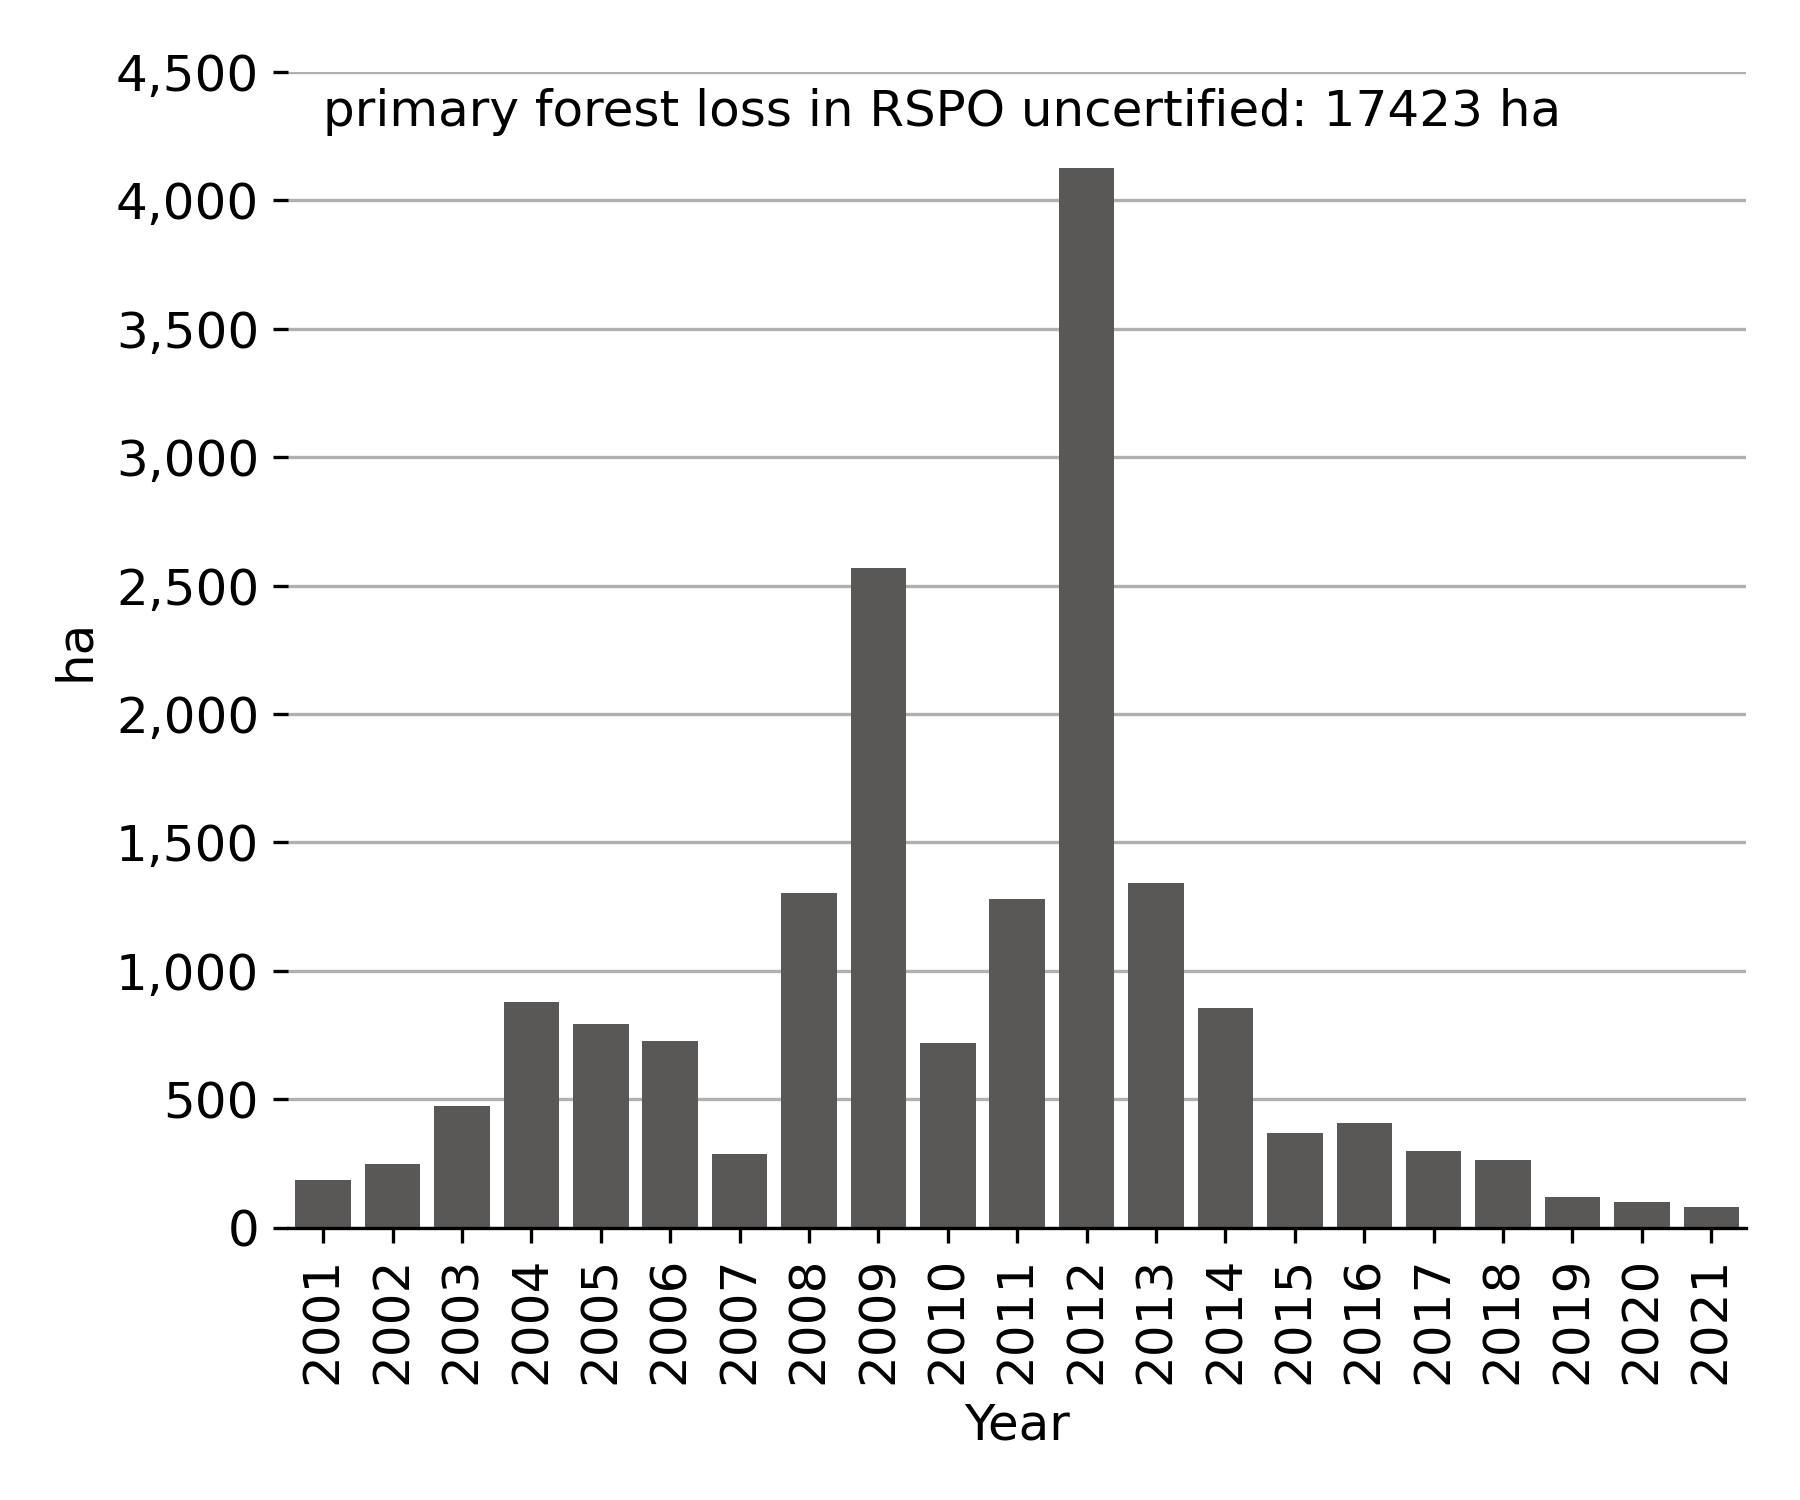
\includegraphics{text/../code/results/final_plots/RSPO_uncertified_primary_loss.png}

}

}

\subcaption{\label{fig-RSPO_secondaryloss}Rates of primary forest loss
within uncertified RSPO concessions, with most occurring between 2008
and 2013.}
\end{minipage}%

\caption{\label{fig-RSPO_forestloss}Difference between primary forest
loss rates in (\textbf{a}) certified and (\textbf{b}) uncertified RSPO
concessions.}

\end{figure}

\hypertarget{infrastructure-1}{%
\section{Infrastructure}\label{infrastructure-1}}

The built up areas have increased by 110\% from 10,332
km\textsuperscript{2} in 2000 to a total of 21,729~km\textsuperscript{2}
in 2020. There was only modest overlap (0.8\%) with forest loss in
primary forests from built up areas in 2000, and more substantial
(17.7\%) with other dense vegetation areas
(Figure~\ref{fig-forestloss_built_up}). These are located either near
existing built up areas (annex IV) or on sites where oil palm was
previously grown.

\begin{figure}

\begin{minipage}[t]{0.50\linewidth}

{\centering 

\raisebox{-\height}{

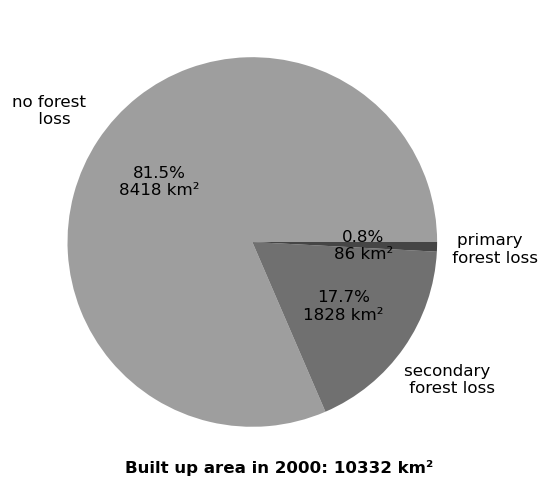
\includegraphics{text/../code/results/final_plots/pie_existing_built_up.png}

}

}

\subcaption{\label{fig-forestloss_pie_existing_built_up}Location of
existing built-up areas in 2000.}
\end{minipage}%
%
\begin{minipage}[t]{0.50\linewidth}

{\centering 

\raisebox{-\height}{

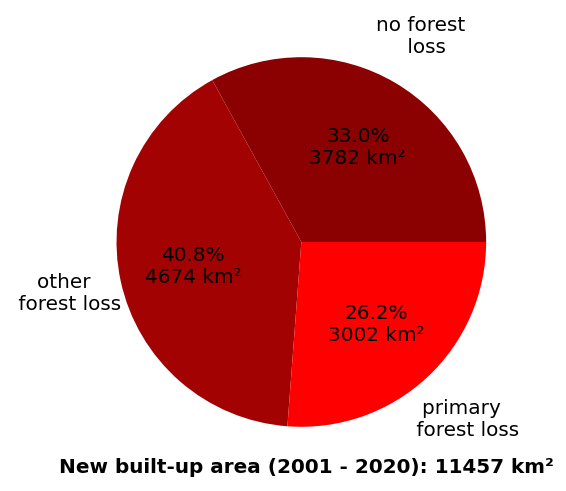
\includegraphics{text/../code/results/final_plots/pie_new_built_up.png}

}

}

\subcaption{\label{fig-forestloss_pie_new_built_up}Location of new
built-up areas in the period between 2001 and 2020..}
\end{minipage}%

\caption{\label{fig-forestloss_built_up}The built-up area within the
study period has more than doubled to a total of 21,789
km\textsuperscript{2}.}

\end{figure}

\hypertarget{primary-forest-loss}{%
\subsection{Primary forest loss}\label{primary-forest-loss}}

Spatial proximity to infrastructure has a direct impact on deforestation
rates, with more than 93.0\% of deforestation occurring within 2000m. It
is evident, that new infrastructure has a higher impact on primary
forest loss than existing. Over 90\% of deforestation happened within
2000 meters of new infrastructure, which only accounts for 57.3 \% of
all primary forest area. This ratio, which is about a factor of 1.6,
increases to a factor of up to 4 within a distance of 100 meters
(Table~\ref{tbl-buffer_primary}). It can also be said that new
infrastructure is built within primary forests, as these buffers cover
more primary forest area than those of existing infrastructure
(Figure~\ref{fig-primary_buffer}). This occurs a lot within the inland
primary forest of Malaysia (Figure~\ref{fig-map_deforestation_primary}).
In addition, new infrastructure lost 22.3\% (100 m) and 14.9\% (200 m)
more forest cover than existing infrastructure.

\begin{figure}

{\centering 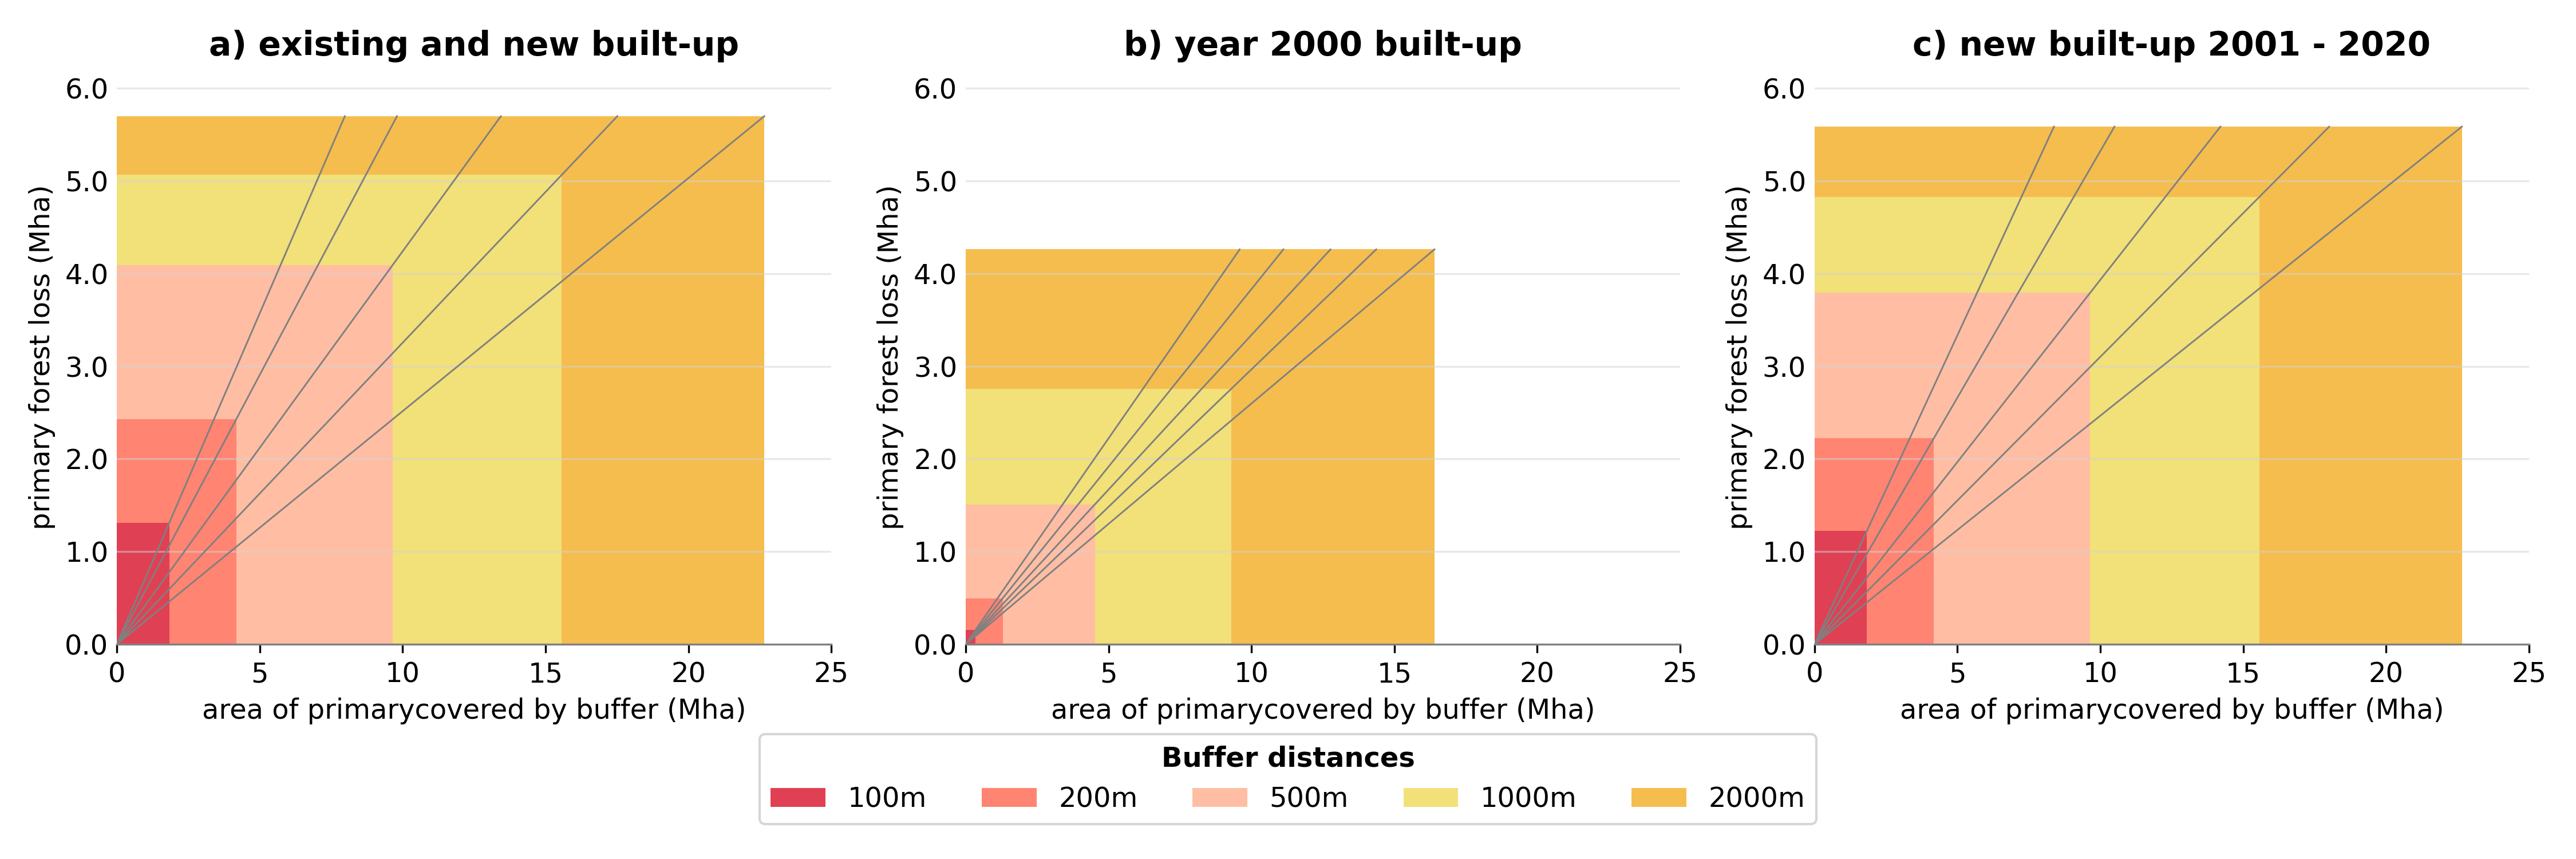
\includegraphics{text/../code/results/final_plots/deforestation_buffer_primary_forest.png}

}

\caption{\label{fig-primary_buffer}The x-axis shows the primary forest
area that falls within the buffer distance. The y-axis shows the amount
of primary forest loss. This shows the relationship of infrastructure
proximity for \textbf{a)} total built-up area 2020 (assumed that no year
2000 areas were removed), \textbf{b)} built-up area in the year 2000 and
\textbf{c)} newly built-up areas between 2000 and 2020.}

\end{figure}

\hypertarget{tbl-buffer_primary}{}
\begin{longtable}[]{@{}
  >{\raggedleft\arraybackslash}p{(\columnwidth - 24\tabcolsep) * \real{0.0667}}
  >{\raggedright\arraybackslash}p{(\columnwidth - 24\tabcolsep) * \real{0.0167}}
  >{\centering\arraybackslash}p{(\columnwidth - 24\tabcolsep) * \real{0.1111}}
  >{\centering\arraybackslash}p{(\columnwidth - 24\tabcolsep) * \real{0.0944}}
  >{\centering\arraybackslash}p{(\columnwidth - 24\tabcolsep) * \real{0.0889}}
  >{\centering\arraybackslash}p{(\columnwidth - 24\tabcolsep) * \real{0.0167}}
  >{\centering\arraybackslash}p{(\columnwidth - 24\tabcolsep) * \real{0.1111}}
  >{\centering\arraybackslash}p{(\columnwidth - 24\tabcolsep) * \real{0.0944}}
  >{\centering\arraybackslash}p{(\columnwidth - 24\tabcolsep) * \real{0.0889}}
  >{\centering\arraybackslash}p{(\columnwidth - 24\tabcolsep) * \real{0.0167}}
  >{\centering\arraybackslash}p{(\columnwidth - 24\tabcolsep) * \real{0.1111}}
  >{\centering\arraybackslash}p{(\columnwidth - 24\tabcolsep) * \real{0.0944}}
  >{\centering\arraybackslash}p{(\columnwidth - 24\tabcolsep) * \real{0.0889}}@{}}
\caption{\label{tbl-buffer_primary}Percentages of primary forest loss
within buffer distances from the total primary forest area. The data is
categorized into three sections: primary forest (portion of the total
primary forest covered by the buffer), loss buffer (portion of forest
loss within total primary forest within buffer area), and loss total
(portion of the loss within buffer from the total primary forest loss).
This is done for \textbf{i)} \emph{total} infrastructure in 2020
(assuming no year 2000 built-up area was removed), \textbf{ii)}
\emph{existing} (year 2000) built up area and \textbf{iii)} \emph{new}
built-up area (2001 - 2020).}\tabularnewline
\toprule\noalign{}
\begin{minipage}[b]{\linewidth}\raggedleft
\textbf{Buffer}
\end{minipage} & \begin{minipage}[b]{\linewidth}\raggedright
\end{minipage} & \begin{minipage}[b]{\linewidth}\centering
\end{minipage} & \begin{minipage}[b]{\linewidth}\centering
\textbf{total}
\end{minipage} & \begin{minipage}[b]{\linewidth}\centering
\end{minipage} & \begin{minipage}[b]{\linewidth}\centering
\end{minipage} & \begin{minipage}[b]{\linewidth}\centering
\end{minipage} & \begin{minipage}[b]{\linewidth}\centering
\textbf{existing}
\end{minipage} & \begin{minipage}[b]{\linewidth}\centering
\end{minipage} & \begin{minipage}[b]{\linewidth}\centering
\end{minipage} & \begin{minipage}[b]{\linewidth}\centering
\end{minipage} & \begin{minipage}[b]{\linewidth}\centering
\textbf{new}
\end{minipage} & \begin{minipage}[b]{\linewidth}\centering
\end{minipage} \\
\midrule\noalign{}
\endfirsthead
\toprule\noalign{}
\begin{minipage}[b]{\linewidth}\raggedleft
\textbf{Buffer}
\end{minipage} & \begin{minipage}[b]{\linewidth}\raggedright
\end{minipage} & \begin{minipage}[b]{\linewidth}\centering
\end{minipage} & \begin{minipage}[b]{\linewidth}\centering
\textbf{total}
\end{minipage} & \begin{minipage}[b]{\linewidth}\centering
\end{minipage} & \begin{minipage}[b]{\linewidth}\centering
\end{minipage} & \begin{minipage}[b]{\linewidth}\centering
\end{minipage} & \begin{minipage}[b]{\linewidth}\centering
\textbf{existing}
\end{minipage} & \begin{minipage}[b]{\linewidth}\centering
\end{minipage} & \begin{minipage}[b]{\linewidth}\centering
\end{minipage} & \begin{minipage}[b]{\linewidth}\centering
\end{minipage} & \begin{minipage}[b]{\linewidth}\centering
\textbf{new}
\end{minipage} & \begin{minipage}[b]{\linewidth}\centering
\end{minipage} \\
\midrule\noalign{}
\endhead
\bottomrule\noalign{}
\endlastfoot
& & \textbf{primary forest} & \textbf{loss buffer} & \textbf{loss total}
& & \textbf{primary forest} & \textbf{loss buffer} & \textbf{loss total}
& & \textbf{primary forest} & \textbf{loss buffer} & \textbf{loss
total} \\
& & & & & & & & & & & & \\
\textbf{100m} & & 4.6 & 71.4 & 21.4 & & 0.9 & 44.4 & 2.5 & & 4.6 & 66.7
& 19.9 \\
\textbf{200m} & & 10.6 & 58.1 & 39.6 & & 3.3 & 38.3 & 8.1 & & 10.6 &
53.2 & 36.3 \\
\textbf{500m} & & 24.4 & 42.4 & 66.7 & & 11.4 & 33.4 & 24.7 & & 24.4 &
39.3 & 61.9 \\
\textbf{1000m} & & 39.6 & 32.5 & 82.7 & & 23.5 & 29.7 & 45.0 & & 39.4 &
31.0 & 78.8 \\
\textbf{2000m} & & 57.3 & 25.2 & 93.0 & & 41.5 & 26.0 & 69.5 & & 57.3 &
24.7 & 91.2 \\
\end{longtable}

\hypertarget{oil-palm-2}{%
\subsection{Oil Palm}\label{oil-palm-2}}

Similarly to primary forest loss, proximity to infrastructure is linked
to new oil palm occurrences. 98.8\% of new oil palms are located within
1000 m of infrastructure (Table~\ref{tbl-buffer_op}). In addition, there
are more new oil palm plantations established within 1000 m of newly
developed areas than within 1000 m of existing infrastructure
(Figure~\ref{fig-op_buffer}).

\begin{figure}

{\centering 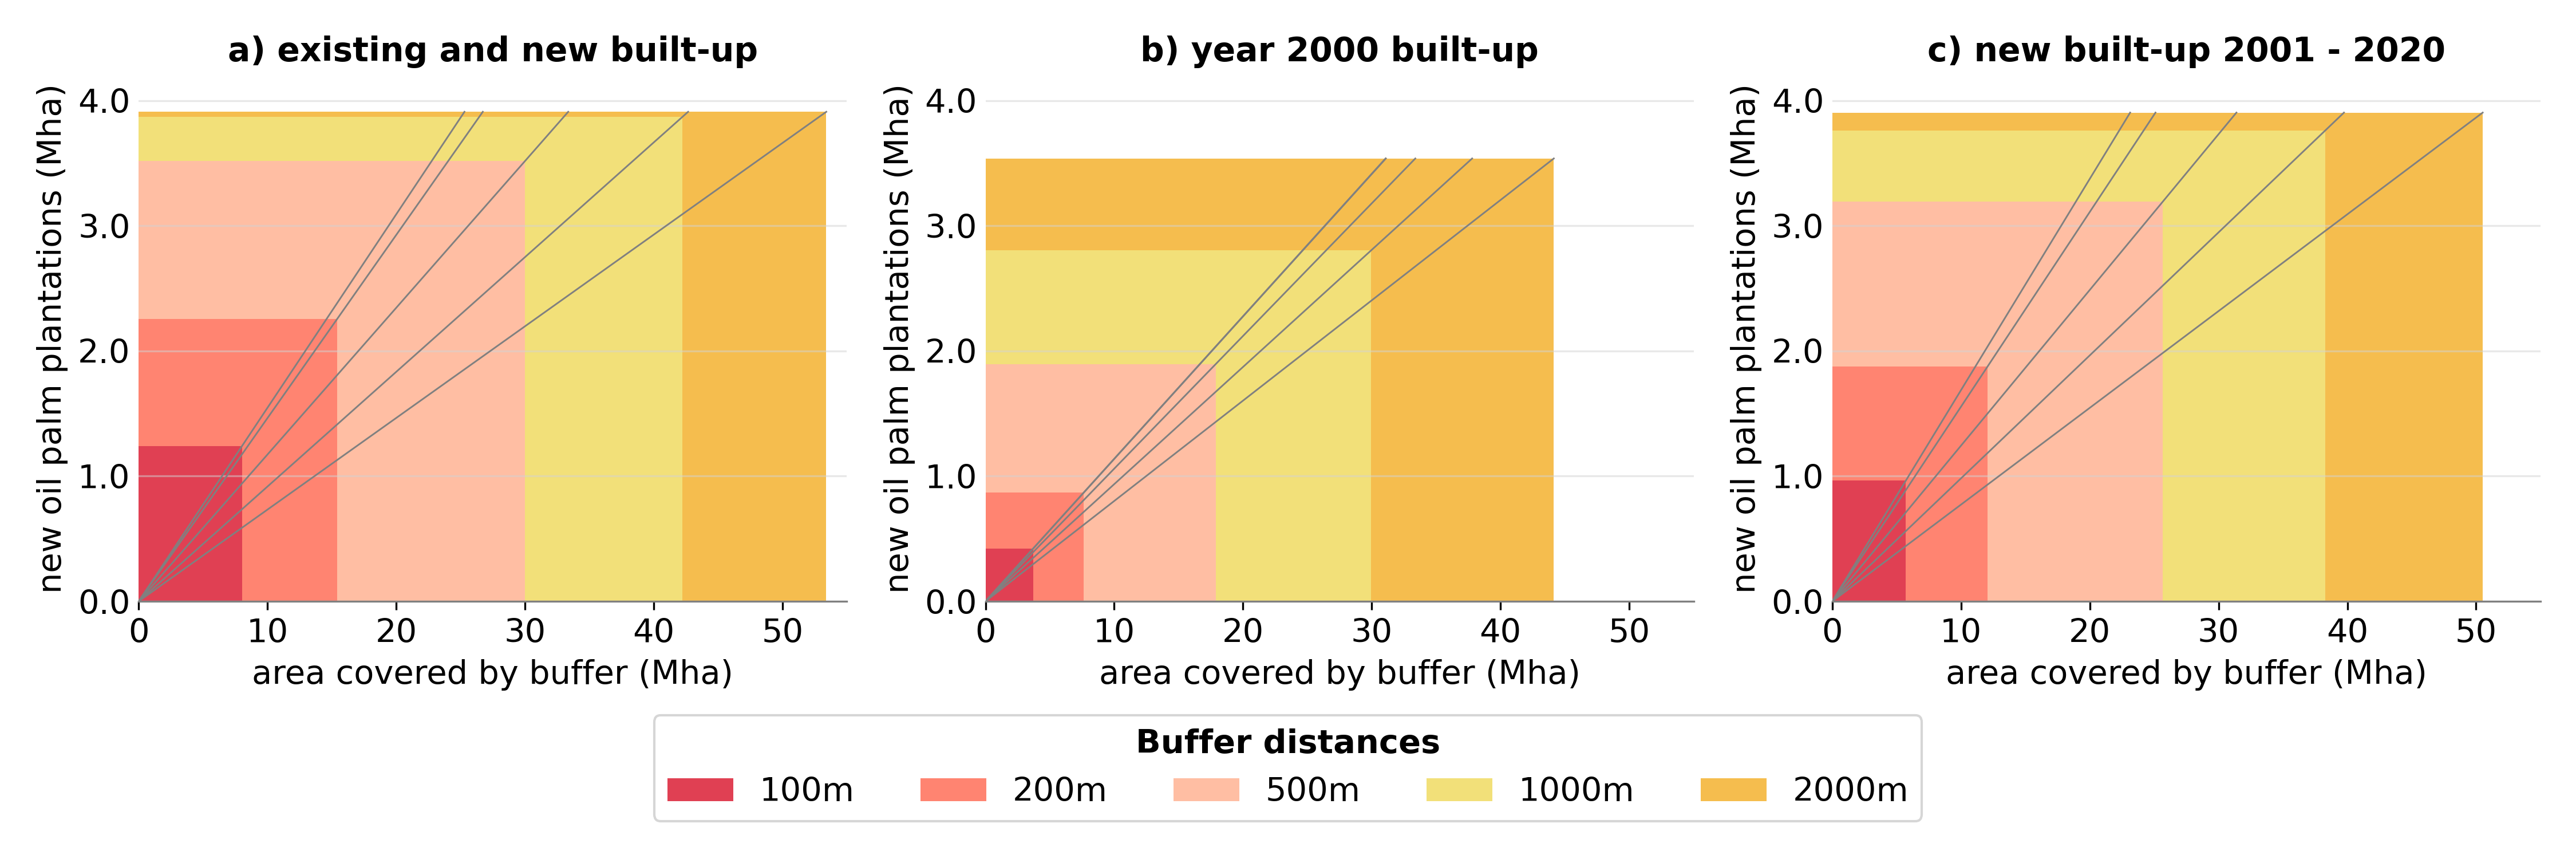
\includegraphics{text/../code/results/final_plots/op_buffer.png}

}

\caption{\label{fig-op_buffer}Composition of vegetated areas on Borneo
at the start of the study period.}

\end{figure}

\newpage

\hypertarget{tbl-buffer_op}{}
\begin{longtable}[]{@{}
  >{\raggedleft\arraybackslash}p{(\columnwidth - 24\tabcolsep) * \real{0.0667}}
  >{\raggedright\arraybackslash}p{(\columnwidth - 24\tabcolsep) * \real{0.0167}}
  >{\centering\arraybackslash}p{(\columnwidth - 24\tabcolsep) * \real{0.1111}}
  >{\centering\arraybackslash}p{(\columnwidth - 24\tabcolsep) * \real{0.1056}}
  >{\centering\arraybackslash}p{(\columnwidth - 24\tabcolsep) * \real{0.0778}}
  >{\centering\arraybackslash}p{(\columnwidth - 24\tabcolsep) * \real{0.0167}}
  >{\centering\arraybackslash}p{(\columnwidth - 24\tabcolsep) * \real{0.1111}}
  >{\centering\arraybackslash}p{(\columnwidth - 24\tabcolsep) * \real{0.1056}}
  >{\centering\arraybackslash}p{(\columnwidth - 24\tabcolsep) * \real{0.0778}}
  >{\centering\arraybackslash}p{(\columnwidth - 24\tabcolsep) * \real{0.0167}}
  >{\centering\arraybackslash}p{(\columnwidth - 24\tabcolsep) * \real{0.1111}}
  >{\centering\arraybackslash}p{(\columnwidth - 24\tabcolsep) * \real{0.1056}}
  >{\centering\arraybackslash}p{(\columnwidth - 24\tabcolsep) * \real{0.0778}}@{}}
\caption{\label{tbl-buffer_op}Percentages of new and existing oil palm
(OP) plantations within buffer distances from the total area of Borneo.
The data is categorized into three sections: area of Borneo (portion of
the total Bornean Area covered by the buffer; excluding buffer areas
that lap over the study extent), new OP buffer (portion newly detected
oil palm from 2001 - 2017 within buffer area), and total OP (portion
newly detected oil palm from 2001 - 2017 from all new oil palm area).
This is done for \textbf{i)} \emph{total} infrastructure in 2020
(assuming no year 2000 built-up area was removed), \textbf{ii)}
\emph{existing} (year 2000) built up area and \textbf{iii)} \emph{new}
built-up area (2001 - 2020).}\tabularnewline
\toprule\noalign{}
\begin{minipage}[b]{\linewidth}\raggedleft
\textbf{Buffer}
\end{minipage} & \begin{minipage}[b]{\linewidth}\raggedright
\end{minipage} & \begin{minipage}[b]{\linewidth}\centering
\end{minipage} & \begin{minipage}[b]{\linewidth}\centering
\textbf{total}
\end{minipage} & \begin{minipage}[b]{\linewidth}\centering
\end{minipage} & \begin{minipage}[b]{\linewidth}\centering
\end{minipage} & \begin{minipage}[b]{\linewidth}\centering
\end{minipage} & \begin{minipage}[b]{\linewidth}\centering
\textbf{existing}
\end{minipage} & \begin{minipage}[b]{\linewidth}\centering
\end{minipage} & \begin{minipage}[b]{\linewidth}\centering
\end{minipage} & \begin{minipage}[b]{\linewidth}\centering
\end{minipage} & \begin{minipage}[b]{\linewidth}\centering
\textbf{new}
\end{minipage} & \begin{minipage}[b]{\linewidth}\centering
\end{minipage} \\
\midrule\noalign{}
\endfirsthead
\toprule\noalign{}
\begin{minipage}[b]{\linewidth}\raggedleft
\textbf{Buffer}
\end{minipage} & \begin{minipage}[b]{\linewidth}\raggedright
\end{minipage} & \begin{minipage}[b]{\linewidth}\centering
\end{minipage} & \begin{minipage}[b]{\linewidth}\centering
\textbf{total}
\end{minipage} & \begin{minipage}[b]{\linewidth}\centering
\end{minipage} & \begin{minipage}[b]{\linewidth}\centering
\end{minipage} & \begin{minipage}[b]{\linewidth}\centering
\end{minipage} & \begin{minipage}[b]{\linewidth}\centering
\textbf{existing}
\end{minipage} & \begin{minipage}[b]{\linewidth}\centering
\end{minipage} & \begin{minipage}[b]{\linewidth}\centering
\end{minipage} & \begin{minipage}[b]{\linewidth}\centering
\end{minipage} & \begin{minipage}[b]{\linewidth}\centering
\textbf{new}
\end{minipage} & \begin{minipage}[b]{\linewidth}\centering
\end{minipage} \\
\midrule\noalign{}
\endhead
\bottomrule\noalign{}
\endlastfoot
& & \textbf{area of Bor.} & \textbf{OP buffer} & \textbf{total OP} & &
\textbf{area of Bor.} & \textbf{OP buffer} & \textbf{total OP} & &
\textbf{area of Bor.} & \textbf{OP buffer} & \textbf{total OP} \\
& & & & & & & & & & & & \\
\textbf{100m} & & 11.0 & 15.5 & 31.7 & & 5.1 & 11.4 & 10.7 & & 7.8 &
16.9 & 24.6 \\
\textbf{200m} & & 21.2 & 14.6 & 57.7 & & 10.5 & 11.4 & 22.2 & & 16.6 &
15.6 & 48.0 \\
\textbf{500m} & & 41.2 & 11.7 & 89.8 & & 24.5 & 10.6 & 48.4 & & 35.2 &
12.4 & 81.6 \\
\textbf{1000m} & & 57.9 & 9.2 & 98.8 & & 41.1 & 9.4 & 71.6 & & 52.6 &
9.8 & 96.1 \\
\textbf{2000m} & & 73.3 & 7.3 & 99.9 & & 60.6 & 8.0 & 90.3 & & 69.3 &
7.7 & 99.7 \\
\end{longtable}

\hypertarget{cropland}{%
\section{Cropland}\label{cropland}}

The land use for non-woody crops increased by 60\% from 0.2 Mha in 2003
to 0.33 Mha in 2019. A quarter of the expansion was at the expense of
previous forest loss (Figure~\ref{fig-croplands}).

\begin{figure}

{\centering 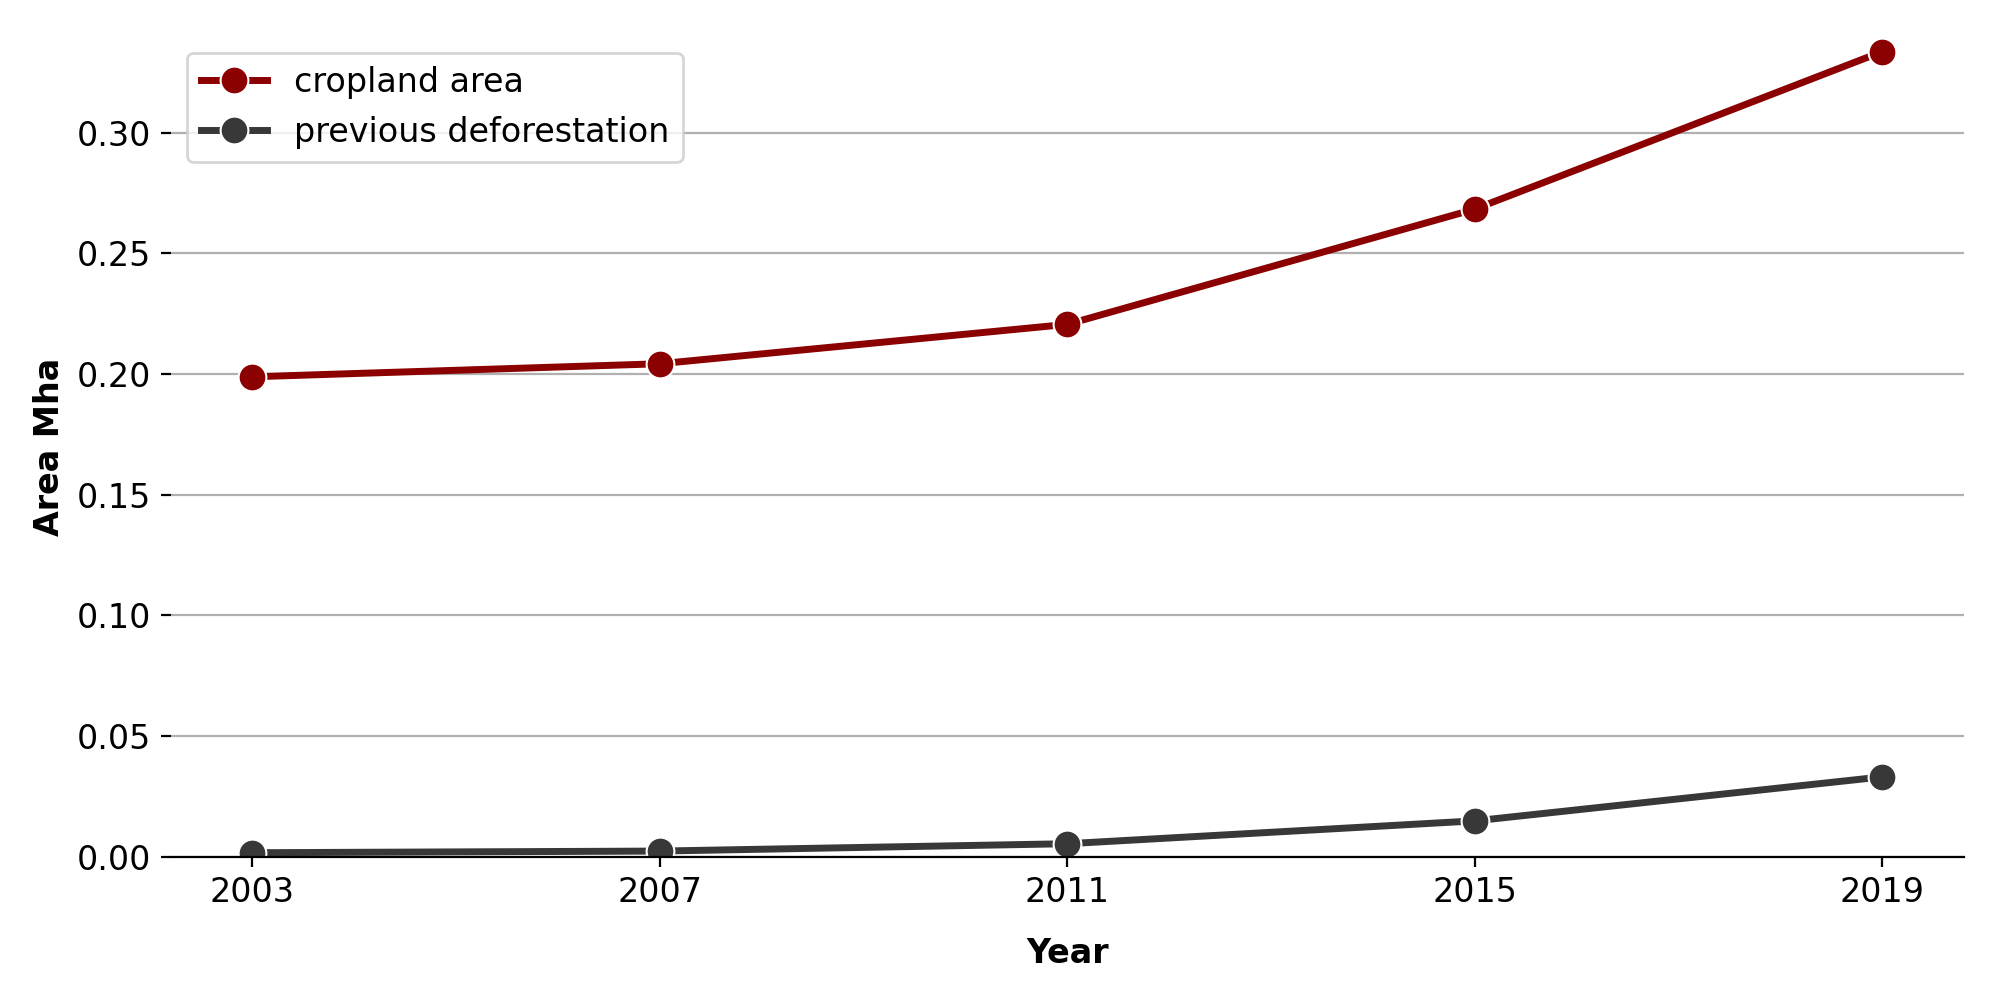
\includegraphics{text/04_literature_review_files/croplands.png}

}

\caption{\label{fig-croplands}Amount of consisten croplands of shrubby
crops.}

\end{figure}

\bookmarksetup{startatroot}

\hypertarget{sec-discussion}{%
\chapter{Discussion}\label{sec-discussion}}

\hypertarget{sec-d_deforestation}{%
\section{Deforestation}\label{sec-d_deforestation}}

Ongoing deforestation in Borneo continues to threaten valuable
biodiversity through further deforestation resulting in habitat loss or
degradation. The declining trend of forest loss in recent years
(Figure~\ref{fig-bardeforestationprimary}) suggests that efforts such as
the moratorium on logging of primary forests in Indonesia are beginning
to have an impact, giving endangered endemic species a chance to be
preserved. Nonetheless, the trend in reduced forest loss must be
confirmed in the coming years to maintain crucial habitat for species
conservation in the long-term. But even if human deforestation continues
to decline, the deforestation that has already happened contributes to
increased fire precursors such as increased temperature, wind speed and
potential evapotranspiration and decreased humidity, cloud cover and
precipitation
(\protect\hyperlink{ref-trancosoConvertingTropicalForests2022}{Trancoso
et al., 2022}). In addition, rising levels of atmospheric
CO\textsubscript{2} are further increasing the risk of wildfires, whilst
also being one of the causes for a phenomenon called El Niño
(\protect\hyperlink{ref-wangHistoricalChangeNino2019}{Wang et al.,
2019}). This event, caused primarily by unusually warm ocean
temperatures, results in significantly higher temperatures during the
dry season, causing the soils to become more dry
(\protect\hyperlink{ref-nasaIndonesianFiresReturn2023}{NASA, 2023};
\protect\hyperlink{ref-wangHistoricalChangeNino2019}{Wang et al.,
2019}). Ultimately, this leads to small-scale fires set by smallholders
to clear pasture spreading much more quickly and across a wider area
(\protect\hyperlink{ref-nasaIndonesianFiresReturn2023}{NASA, 2023}).
Therefore, the small-scale fires occurring all over Borneo can not only
be attributed to smallholders, but they are also the trigger for the
large-scale fires, which are fueled by the El Niño phenomenon and the
reason for the outlier years with a lot more forest fires, including
those in protected areas. Nevertheless, the low rates of deforestation
in protected areas emphasize their importance. This suggests that
additional protected areas could be an important tool to ensure the
integrity of the relatively untouched primary forests in the inland of
Borneo. Additionally, smallholders should be sensitized or at least
alarmed, if an El Nino year approaches, to reduce the risk of future
large forest fires, especially close to protected areas.

\hypertarget{oil-palm-3}{%
\section{Oil Palm}\label{oil-palm-3}}

Whilst this thesis allocates \textasciitilde4 Mha to newly detected oil
palm plantations on Borneo from 2001 to 2017, another paper states a
higher number with \textasciitilde{} 5.5 Mha for the same period
(\protect\hyperlink{ref-gaveauRiseFallForest2019}{Gaveau et al., 2019}).
Gaveau et al.~only defined industrial plantation \textgreater90ha on
satellite imagery by eye
(\protect\hyperlink{ref-gaveauRiseFallForest2019}{2019}). Considering
the 4-year detection lag of the remotely sensed dataset and the yearly
detection rate in these years (\textasciitilde0.3 Mha), the results
coincide. However, the data used here is based on a remote sensing
approach and includes smallholder plantations, and therefore it is
likely that the newly discovered oil palms are underestimated. This is
further supported by the fact that many oil palm plantations are located
on deforestation clusters that are not completely covered by oil palms
(Figure~\ref{fig-map_deforestation_op_fires}). Thus, it can be concluded
that the numbers on oil palm and subsequently deforestation prior to oil
palm plantations are too low.

Even though Danylo et al.~state, that it takes only 2-3 years for newly
planted oil palms to be detected
(\protect\hyperlink{ref-danyloMapExtentYear2021}{2021}), the lag phase
in Figure~\ref{fig-bar_opdeforestation} indicates, that it is 4-5 years.
As oil palm plantations in primary forests (0.71 Mha) account for 21.4\%
of all primary forest logging (excluding forest fires) from 2001 to 2013
(3.31 Mha) and considering the underestimation of new oil palms, it can
be concluded, that oil palm is an important driver of primary forest
loss on Borneo. Nonetheless, even if other areas of primary forest loss
would account for conversion to other industrial plantations, this still
makes logging the main driver of primary forest loss.

The portion of new oil palm on secondary forest loss areas did not
necessarily completely replace forests. Since oil palm plantations need
to be replanted (see Section~\ref{sec-oilpalm}), but are also
categorized as secondary forest, replanting is categorized as secondary
forest loss. Additionally, it would be too facile to attribute all of
the deforestation solely to palm oil, since it is not known whether oil
palm caused deforestation or merely followed the clearing of land
(\protect\hyperlink{ref-fitzherbertHowWillOil2008}{Fitzherbert et al.,
2008}). For example, some companies used palm oil concessions to obtain
permission to log, and thus make money, without cultivating palm oil on
the land (\protect\hyperlink{ref-fitzherbertHowWillOil2008}{Fitzherbert
et al., 2008}). However, it is not known if this practice still exists
and planting of oil palms is reported to be detected immediately after
clearing (\protect\hyperlink{ref-gaveauRiseFallForest2019}{Gaveau et
al., 2019}). In addition, the fine-scaled unorganized patterns for
logging (see Figure~\ref{fig-map_deforestation_primary}) differ strongly
from the rectangle, clear edge and large area clearing (see
Figure~\ref{fig-map_deforestation_op_fires}).

Even though plantation expansion has slowed, the recent large price jump
(from 601 USD per ton in 2019 to 1276 USD in 2022) is a worrying
indicator, that this trend will soon be reversed in the future
(\protect\hyperlink{ref-worldbankAveragePricesPalm2023}{World Bank,
2023}). This is because the price is closely linked to the expansion of
oil palm production
(\protect\hyperlink{ref-gaveauSlowingDeforestationIndonesia2022}{Gaveau
et al., 2022}) and thus to environmental issues discussed in
Section~\ref{sec-oilpalm}.

\hypertarget{rspo}{%
\subsection{RSPO}\label{rspo}}

While, based on the data information given by the RSPO, it remains
unclear what an uncertified RSPO concession is, certified concessions
represent with 15.8\% roughly the share of the RSPO certified palm oil
trade (19\%, see Section~\ref{sec-rspo}). Since most of the concessions
are located on predominantly deforested land anyway, it can be said that
the palm oil coming from these plantations does not further contribute
to a noteworthy loss of primary forest, since no blending takes place in
the mills, which is strictly regulated by RSPO regulations
(\protect\hyperlink{ref-rspoRSPOPrinciplesCriteria2018}{RSPO, 2018}).

Although primary forests take up a marginal amount of RSPO concessions
and much of it is already logged (Section~\ref{sec-resultsrspo}), the
sharp drop in primary deforestation within certified concessions in 2011
(Figure~\ref{fig-RSPO_primaryloss}) is still remarkable, as it coincides
with the introduction of the Indonesian moratorium of logging in primary
forest. Nevertheless, it would be highly uncertain to assume a link here
due to i) the small reference area and ii) the fact that RSPO concession
data is only available for Malaysia.

A statement on whether the introduction of the RSPO label has reduced
deforestation by palm oil overall cannot be made and would also be an
exaggeration since the RSPO has no or at best indirect influence via
advising politicians on concessions for new palm oil plantations. In
summary, despite the criticism directed at the RSPO (see
Section~\ref{sec-rspo}), it must be said that at least no more primary
forest is being lost for their certified palm oil.

\hypertarget{infrastructure-2}{%
\section{Infrastructure}\label{infrastructure-2}}

If both the built up area and the forest loss datased had 100\%
accuracy, there should not be any deforestation on built up areas from
2000. Whilst the marginal 0.8\% overlap with primary forest clearing
confirms high accuracy, the 17.7\% with secondary forest cannot be
attributed to data inaccuracy (see
Figure~\ref{fig-forestloss_pie_existing_built_up}). The reason for this
unexpectedly large number can be assigned to maintenance work of
constantly overgrowing vegetation near roads (see annex IV).

\hypertarget{buffer}{%
\subsection{Buffer}\label{buffer}}

With almost three quarters of the Bornean land within 2000 m of
infrastructure in 2020, accessibility of remote areas has increased by
92557km \textsuperscript{2} over the study period, leaving only 26.7\%
of Borneo untouched (Table~\ref{tbl-buffer_op}). This increases the
pollution pressures described in Section~\ref{sec-infrastructure}.
However, as the underlying dataset does not separate private roads
(e.g.~maintenance roads for industrial plantations) from public roads,
it remains unclear how much of the increase in accessibility is due to
the expansion of public infrastructure versus private development.
However, more detailed maps that capture the temporal development of new
roads are scarce. Only open street map provides access to historical
data going back to 2013, but its completeness depends on the activity of
the users and is therefore questionable, especially in early years.
Therefore, a new dataset covering infrastructure development (especially
roads) in an annual interval would be an important tool for further
research in quantifying the impact of new infrastructure. Nevertheless,
the relationship between the establishment of new oil palm plantations
and deforestation rates could be closely linked to better access through
new infrastructure (Table~\ref{tbl-buffer_primary},
Table~\ref{tbl-buffer_op}). Hence, it is crucial to implement
sustainable infrastructure development practices and stringent
regulations to mitigate the disturbance effects of future infrastructure
projects, especially with respect to the planned relocation of the
Indonesian capital to Borneo, where Indonesia has the chance to set new
standards for sustainable infrastructure development in the tropics
(\protect\hyperlink{ref-spencerImplicationsLargescaleInfrastructure2023}{Spencer
et al., 2023}).

Another often overlooked form of infrastructure are natural waterways,
which allow easy access deep into the forests. Thus, the deforestation
of primary forest along rivers (see annex V) can also be attributed to
(natural) infrastructure.

\hypertarget{cropland-1}{%
\section{Cropland}\label{cropland-1}}

Due to the small amount of acreage devoted to shrubby crops, their share
of deforestation is almost negligible compared to palm oil. However,
there are many small wildfires near these croplands, supporting the
claim that smallholders are using fire to clear the land near their
fields for pasture, which has a high risk of triggering large-scale
wildfires (Section~\ref{sec-d_deforestation}).

Although other tree crops are grown on Borneo in addition to oil palm,
they - even though understudied - certainly do not reach anywhere near
the scale of oil palm plantations, with Gaveau et al.~reporting that oil
palm accounts for 88\% of industrial plantations in Borneo
(\protect\hyperlink{ref-gaveauRiseFallForest2019}{2019}).

\hypertarget{conclusions}{%
\section{Conclusions}\label{conclusions}}

In summary, Borneo continues to be threatened by deforestation, which
endangers its unique biodiversity and habitat integrity. Recent figures
show a declining trend in forest loss, likely due to initiatives such as
the moratorium on logging in Indonesia's primary forests. However, this
trend requires continued confirmation to prof long-term conservation
efforts. Furthermore, rising atmospheric CO2 levels and the El Niño
phenomenon increase forest fire risk. Protected areas play an important
role in maintaining primary forests and biodiversity.

The expansion of oil palm cultivation, which is the second largest
contributor to primary forest loss after logging, is showing signs of
slowing, although the recent rise in palm oil prices is an alarming
indicator. Since 2011, virtually no primary forest has been cut down for
RSPO-certified palm oil, making it, despite criticism and the lack of
alternative labels, the most viable option for sustainably conscious
stakeholders at present. Other crops only play a minor role in
deforestation. Infrastructure development has substantially improved
accessibility to remote areas, which led to increased deforestation,
hence calling for sustainable practices and strict regulations for
future projects.

In summary, the problem of deforestation in Borneo can only be addressed
with a holistic approach that includes sustainable practices, strict
regulations, awareness campaigns, and responsible development to protect
the exceptional biodiversity within the remaining primary forests.

\bookmarksetup{startatroot}

\hypertarget{references}{%
\chapter{References}\label{references}}

\hypertarget{refs}{}
\begin{CSLReferences}{1}{0}
\leavevmode\vadjust pre{\hypertarget{ref-abdulmajidSustainablePalmOil2021}{}}%
Abdul Majid, N., Ramli, Z., Md Sum, S., \& Awang, A. H. (2021).
Sustainable {Palm Oil Certification Scheme Frameworks} and {Impacts}: {A
Systematic Literature Review}. \emph{Sustainability}, \emph{13}(6),
3263. \url{https://doi.org/10.3390/su13063263}

\leavevmode\vadjust pre{\hypertarget{ref-alamgirHighriskInfrastructureProjects2019}{}}%
Alamgir, M., Campbell, M. J., Sloan, S., Suhardiman, A., Supriatna, J.,
\& Laurance, W. F. (2019). High-risk infrastructure projects pose
imminent threats to forests in {Indonesian Borneo}. \emph{Scientific
Reports}, \emph{9}(1), 140.
\url{https://doi.org/10.1038/s41598-018-36594-8}

\leavevmode\vadjust pre{\hypertarget{ref-austinWhatCausesDeforestation2019}{}}%
Austin, K. G., Schwantes, A., Gu, Y., \& Kasibhatla, P. S. (2019). What
causes deforestation in {Indonesia}? \emph{Environmental Research
Letters}, \emph{14}(2), 024007.
\url{https://doi.org/10.1088/1748-9326/aaf6db}

\leavevmode\vadjust pre{\hypertarget{ref-barnesConsequencesTropicalLand2014}{}}%
Barnes, A. D., Jochum, M., Mumme, S., Haneda, N. F., Farajallah, A.,
Widarto, T. H., \& Brose, U. (2014). Consequences of tropical land use
for multitrophic biodiversity and ecosystem functioning. \emph{Nature
Communications}, \emph{5}(1), 5351.
\url{https://doi.org/10.1038/ncomms6351}

\leavevmode\vadjust pre{\hypertarget{ref-basironOILPALMITS2004}{}}%
Basiron, Y., \& Weng, C. K. (2004). {THE OIL PALM AND ITS
SUSTAINABILITY}. \emph{JOURNAL OF OIL PALM RESEARCH}.

\leavevmode\vadjust pre{\hypertarget{ref-boeingOSMnxPythonPackage2017}{}}%
Boeing, G. (2017). \emph{{OSMnx}: {A Python} package to work with
graph-theoretic {OpenStreetMap} street networks}.
\url{https://doi.org/DOI:10.21105/joss.00215}

\leavevmode\vadjust pre{\hypertarget{ref-buschReductionsEmissionsDeforestation2015}{}}%
Busch, J., Ferretti-Gallon, K., Engelmann, J., Wright, M., Austin, K.
G., Stolle, F., Turubanova, S., Potapov, P. V., Margono, B., Hansen, M.
C., \& Baccini, A. (2015). Reductions in emissions from deforestation
from {Indonesia}'s moratorium on new oil palm, timber, and logging
concessions. \emph{Proceedings of the National Academy of Sciences},
\emph{112}(5), 1328--1333. \url{https://doi.org/10.1073/pnas.1412514112}

\leavevmode\vadjust pre{\hypertarget{ref-byerleeTropicalOilCrop2016}{}}%
Byerlee, D., Falcon, W. P., \& Naylor, R. L. (2016). \emph{The {Tropical
Oil Crop Revolution}: {Food}, {Feed}, {Fuel}, and {Forests}}. {Oxford
University Press}.
\url{https://doi.org/10.1093/acprof:oso/9780190222987.001.0001}

\leavevmode\vadjust pre{\hypertarget{ref-cazzollagattiSustainablePalmOil2019}{}}%
Cazzolla Gatti, R., Liang, J., Velichevskaya, A., \& Zhou, M. (2019).
Sustainable palm oil may not be so sustainable. \emph{Science of The
Total Environment}, \emph{652}, 48--51.
\url{https://doi.org/10.1016/j.scitotenv.2018.10.222}

\leavevmode\vadjust pre{\hypertarget{ref-changEconomicPerspectiveOil2003}{}}%
Chang, E. S., Abdul Rahim, A. S., \& Zainon, B. (2003). \emph{An
{Economic Perspective} of {Oil Extraction Rate} in the {Oil Palm
Industry} of {Malaysia}}. \emph{3}(1), 25--31.

\leavevmode\vadjust pre{\hypertarget{ref-chewImprovingSustainabilityPalm2021}{}}%
Chew, C. L., Ng, C. Y., Hong, W. O., Wu, T. Y., Lee, Y.-Y., Low, L. E.,
Kong, P. S., \& Chan, E. S. (2021). Improving {Sustainability} of {Palm
Oil Production} by {Increasing Oil Extraction Rate}: A {Review}.
\emph{Food and Bioprocess Technology}, \emph{14}(4), 573--586.
\url{https://doi.org/10.1007/s11947-020-02555-1}

\leavevmode\vadjust pre{\hypertarget{ref-coetzeeOpenGeospatialSoftware2020}{}}%
Coetzee, S., Ivánová, I., Mitasova, H., \& Brovelli, M. (2020). Open
{Geospatial Software} and {Data}: {A Review} of the {Current State} and
{A Perspective} into the {Future}. \emph{ISPRS International Journal of
Geo-Information}, \emph{9}(2), 90.
\url{https://doi.org/10.3390/ijgi9020090}

\leavevmode\vadjust pre{\hypertarget{ref-crowleyRemoteSensingRecent2020}{}}%
Crowley, M. A., \& Cardille, J. A. (2020). Remote {Sensing}'s {Recent}
and {Future Contributions} to {Landscape Ecology}. \emph{Current
Landscape Ecology Reports}, \emph{5}(3), 45--57.
\url{https://doi.org/10.1007/s40823-020-00054-9}

\leavevmode\vadjust pre{\hypertarget{ref-curtisClassifyingDriversGlobal2018}{}}%
Curtis, P. G., Slay, C. M., Harris, N. L., Tyukavina, A., \& Hansen, M.
C. (2018). Classifying drivers of global forest loss. \emph{Science},
\emph{361}(6407), 1108--1111.
\url{https://doi.org/10.1126/science.aau3445}

\leavevmode\vadjust pre{\hypertarget{ref-danyloMapExtentYear2021}{}}%
Danylo, O., Pirker, J., Lemoine, G., Ceccherini, G., See, L., McCallum,
I., Hadi, Kraxner, F., Achard, F., \& Fritz, S. (2021). A map of the
extent and year of detection of oil palm plantations in {Indonesia},
{Malaysia} and {Thailand}. \emph{Scientific Data}, \emph{8}(1), 96.
\url{https://doi.org/10.1038/s41597-021-00867-1}

\leavevmode\vadjust pre{\hypertarget{ref-darRoadsActCorridors2015}{}}%
Dar, P. A., Reshi, Z. A., \& Shah, M. A. (2015). \emph{Roads act as
corridors for the spread of alien plant species in the mountainous
regions: {A} case study of {Kashmir Valley}, {India}}.

\leavevmode\vadjust pre{\hypertarget{ref-descalsHighresolutionGlobalMap2021}{}}%
Descals, A., Wich, S., Meijaard, E., Gaveau, D. L. A., Peedell, S., \&
Szantoi, Z. (2021). High-resolution global map of smallholder and
industrial closed-canopy oil palm plantations. \emph{Earth System
Science Data}, \emph{13}(3), 1211--1231.
\url{https://doi.org/10.5194/essd-13-1211-2021}

\leavevmode\vadjust pre{\hypertarget{ref-didhamRethinkingConceptualFoundations2012a}{}}%
Didham, R. K., Kapos, V., \& Ewers, R. M. (2012). Rethinking the
conceptual foundations of habitat fragmentation research. \emph{Oikos},
\emph{121}(2), 161--170.
\url{https://doi.org/10.1111/j.1600-0706.2011.20273.x}

\leavevmode\vadjust pre{\hypertarget{ref-eiaWhoWatchesWatchmen2015}{}}%
EIA. (2015). \emph{Who watches the watchmen?}

\leavevmode\vadjust pre{\hypertarget{ref-esriQuick_Notes_on_Map_Projections_in_ArcGIS_nov2019Pdf2019}{}}%
esri. (2019).
\emph{Quick\_{Notes}\_on\_{Map}\_{Projections}\_in\_{ArcGIS}\_nov2019.pdf}.

\leavevmode\vadjust pre{\hypertarget{ref-esriLambertAzimuthalEqualarea2023}{}}%
esri. (2023). \emph{Lambert azimuthal
equal-area\textemdash{{ArcGIS Pro}} \textbar{} {Documentation}}.
https://pro.arcgis.co
m/en/pro-app/latest/help/mapping/properties/lambert-azimuthal-equal-area.htm.

\leavevmode\vadjust pre{\hypertarget{ref-fahrigRethinkingPatchSize2013}{}}%
Fahrig, L. (2013). Rethinking patch size and isolation effects: The
habitat amount hypothesis. \emph{Journal of Biogeography}, \emph{40}(9),
1649--1663. \url{https://doi.org/10.1111/jbi.12130}

\leavevmode\vadjust pre{\hypertarget{ref-faoGlobalForestResources2020}{}}%
FAO. (2020). \emph{Global {Forest Resources Assessment} 2020}. {FAO}.
\url{https://doi.org/10.4060/ca9825en}

\leavevmode\vadjust pre{\hypertarget{ref-faoFAOSTATDatabase2023}{}}%
FAO. (2023). \emph{{FAOSTAT Database}}.
https://www.fao.org/faostat/en/\#compare.

\leavevmode\vadjust pre{\hypertarget{ref-fitzherbertHowWillOil2008}{}}%
Fitzherbert, E., Struebig, M., Morel, A., Danielsen, F., Bruhl, C.,
Donald, P., \& Phalan, B. (2008). How will oil palm expansion affect
biodiversity? \emph{Trends in Ecology \& Evolution}, \emph{23}(10),
538--545. \url{https://doi.org/10.1016/j.tree.2008.06.012}

\leavevmode\vadjust pre{\hypertarget{ref-foleySolutionsCultivatedPlanet2011}{}}%
Foley, J. A., Ramankutty, N., Brauman, K. A., Cassidy, E. S., Gerber, J.
S., Johnston, M., Mueller, N. D., O'Connell, C., Ray, D. K., West, P.
C., Balzer, C., Bennett, E. M., Carpenter, S. R., Hill, J., Monfreda,
C., Polasky, S., Rockström, J., Sheehan, J., Siebert, S., \ldots{} Zaks,
D. P. M. (2011). Solutions for a cultivated planet. \emph{Nature},
\emph{478}(7369), 337--342. \url{https://doi.org/10.1038/nature10452}

\leavevmode\vadjust pre{\hypertarget{ref-gaveauSlowingDeforestationIndonesia2022}{}}%
Gaveau, D. L. A., Locatelli, B., Salim, M. A., Husnayaen, Manurung, T.,
Descals, A., Angelsen, A., Meijaard, E., \& Sheil, D. (2022). Slowing
deforestation in {Indonesia} follows declining oil palm expansion and
lower oil prices. \emph{PLOS ONE}, \emph{17}(3), e0266178.
\url{https://doi.org/10.1371/journal.pone.0266178}

\leavevmode\vadjust pre{\hypertarget{ref-gaveauRiseFallForest2019}{}}%
Gaveau, D. L. A., Locatelli, B., Salim, M. A., Yaen, H., Pacheco, P., \&
Sheil, D. (2019). Rise and fall of forest loss and industrial
plantations in {Borneo} (2000\textendash 2017). \emph{Conservation
Letters}, \emph{12}(3), e12622. \url{https://doi.org/10.1111/conl.12622}

\leavevmode\vadjust pre{\hypertarget{ref-gaveauFourDecadesForest2014}{}}%
Gaveau, D. L. A., Sloan, S., Molidena, E., Yaen, H., Sheil, D., Abram,
N. K., Ancrenaz, M., Nasi, R., Quinones, M., Wielaard, N., \& Meijaard,
E. (2014). Four {Decades} of {Forest Persistence}, {Clearance} and
{Logging} on {Borneo}. \emph{PLoS ONE}, \emph{9}(7), e101654.
\url{https://doi.org/10.1371/journal.pone.0101654}

\leavevmode\vadjust pre{\hypertarget{ref-gilliesRasterioDocumentation2023}{}}%
Gillies, S. (2023). \emph{Rasterio {Documentation}}.

\leavevmode\vadjust pre{\hypertarget{ref-greenpeaceinternationalCertifyingDestruction2013}{}}%
Greenpeace International. (2013). \emph{Certifying destruction}.

\leavevmode\vadjust pre{\hypertarget{ref-groganGlobalGriddedCrop2022}{}}%
Grogan, D., Frolking, S., Wisser, D., Prusevich, A., \& Glidden, S.
(2022). Global gridded crop harvested area, production, yield, and
monthly physical area data circa 2015. \emph{Scientific Data},
\emph{9}(1), 15. \url{https://doi.org/10.1038/s41597-021-01115-2}

\leavevmode\vadjust pre{\hypertarget{ref-haddadHabitatFragmentationIts2015a}{}}%
Haddad, N. M., Brudvig, L. A., Clobert, J., Davies, K. F., Gonzalez, A.,
Holt, R. D., Lovejoy, T. E., Sexton, J. O., Austin, M. P., Collins, C.
D., Cook, W. M., Damschen, E. I., Ewers, R. M., Foster, B. L., Jenkins,
C. N., King, A. J., Laurance, W. F., Levey, D. J., Margules, C. R.,
\ldots{} Townshend, J. R. (2015). Habitat fragmentation and its lasting
impact on {Earth}'s ecosystems. \emph{Science Advances}, \emph{1}(2),
e1500052. \url{https://doi.org/10.1126/sciadv.1500052}

\leavevmode\vadjust pre{\hypertarget{ref-hadiyantoPhytoremediationsPalmOil2013}{}}%
Hadiyanto, H., Christward, M., \& Soetrisnan, D. (2013).
Phytoremediations of {Palm Oil Mill Effluent} ({POME}) by {Using Aquatic
Plants} and {Microalge} for {Biomass Production}. \emph{Journal of
Environmental Science and Technology}, \emph{6}(2), 79--90.
\url{https://doi.org/10.3923/jest.2013.79.90}

\leavevmode\vadjust pre{\hypertarget{ref-hansenHighResolutionGlobalMaps2013}{}}%
Hansen, M. C., Potapov, P. V., Moore, R., Hancher, M., Turubanova, S.
A., Tyukavina, A., Thau, D., Stehman, S. V., Goetz, S. J., Loveland, T.
R., Kommareddy, A., Egorov, A., Chini, L., Justice, C. O., \& Townshend,
J. R. G. (2013). High-{Resolution Global Maps} of 21st-{Century Forest
Cover Change}. \emph{Science}, \emph{342}(6160), 850--853.
\url{https://doi.org/10.1126/science.1244693}

\leavevmode\vadjust pre{\hypertarget{ref-harrisArrayProgrammingNumPy2020}{}}%
Harris, C. R., Millman, K. J., Van Der Walt, S. J., Gommers, R.,
Virtanen, P., Cournapeau, D., Wieser, E., Taylor, J., Berg, S., Smith,
N. J., Kern, R., Picus, M., Hoyer, S., Van Kerkwijk, M. H., Brett, M.,
Haldane, A., Del Río, J. F., Wiebe, M., Peterson, P., \ldots{} Oliphant,
T. E. (2020). Array programming with {NumPy}. \emph{Nature},
\emph{585}(7825), 357--362.
\url{https://doi.org/10.1038/s41586-020-2649-2}

\leavevmode\vadjust pre{\hypertarget{ref-harrisonTropicalForestPeatland2020}{}}%
Harrison, M. E., Ottay, J. B., D'Arcy, L. J., Cheyne, S. M., Anggodo,
Belcher, C., Cole, L., Dohong, A., Ermiasi, Y., Feldpausch, T.,
Gallego-Sala, A., Gunawan, A., Höing, A., Husson, S. J., Kulu, I. P.,
Soebagio, S. M., Mang, S., Mercado, L., Morrogh-Bernard, H. C., \ldots{}
Van Veen, F. J. F. (2020). Tropical forest and peatland conservation in
{Indonesia}: {Challenges} and directions. \emph{People and Nature},
\emph{2}(1), 4--28. \url{https://doi.org/10.1002/pan3.10060}

\leavevmode\vadjust pre{\hypertarget{ref-houghtonEmissionsCarbonDeforestation2013}{}}%
Houghton, R. A. (2013). The emissions of carbon from deforestation and
degradation in the tropics: Past trends and future potential.
\emph{Carbon Management}, \emph{4}(5), 539--546.
\url{https://doi.org/10.4155/cmt.13.41}

\leavevmode\vadjust pre{\hypertarget{ref-ieaGlobalLandTransport2013}{}}%
IEA. (2013). \emph{Global {Land Transport Infrastructure Requirements}}.

\leavevmode\vadjust pre{\hypertarget{ref-iucnPongoPygmaeusAncrenaz2016}{}}%
IUCN. (2016). \emph{Pongo pygmaeus: {Ancrenaz}, {M}., {Gumal}, {M}.,
{Marshall}, {A}.{J}., {Meijaard}, {E}., {Wich} , {S}.{A}. \& {Husson},
{S}.: {The IUCN Red List} of {Threatened Species} 2016:
E.{T17975A123809220}}. {International Union for Conservation of Nature}.
\url{https://doi.org/10.2305/IUCN.UK.2016-1.RLTS.T17975A17966347.en}

\leavevmode\vadjust pre{\hypertarget{ref-jaureguiberryDirectDriversRecent2022}{}}%
Jaureguiberry, P., Titeux, N., Wiemers, M., Bowler, D. E., Coscieme, L.,
Golden, A. S., Guerra, C. A., Jacob, U., Takahashi, Y., Settele, J.,
Díaz, S., Molnár, Z., \& Purvis, A. (2022). The direct drivers of recent
global anthropogenic biodiversity loss. \emph{Science Advances},
\emph{8}(45), eabm9982. \url{https://doi.org/10.1126/sciadv.abm9982}

\leavevmode\vadjust pre{\hypertarget{ref-jenkinsGlobalPatternsTerrestrial2013}{}}%
Jenkins, C. N., Pimm, S. L., \& Joppa, L. N. (2013). Global patterns of
terrestrial vertebrate diversity and conservation. \emph{Proceedings of
the National Academy of Sciences}, \emph{110}(28).
\url{https://doi.org/10.1073/pnas.1302251110}

\leavevmode\vadjust pre{\hypertarget{ref-jeongPerformanceComparisonMesophilic2014}{}}%
Jeong, J.-Y., Son, S.-M., Pyon, J.-H., \& Park, J.-Y. (2014).
Performance comparison between mesophilic and thermophilic anaerobic
reactors for treatment of palm oil mill effluent. \emph{Bioresource
Technology}, \emph{165}, 122--128.
\url{https://doi.org/10.1016/j.biortech.2014.04.007}

\leavevmode\vadjust pre{\hypertarget{ref-kamyabElaeisGuineensis2022}{}}%
Kamyab, H. (Ed.). (2022). \emph{Elaeis guineensis}. {IntechOpen}.
\url{https://doi.org/10.5772/intechopen.92931}

\leavevmode\vadjust pre{\hypertarget{ref-karraGlobalLandUse2021}{}}%
Karra, K., Kontgis, C., Statman-Weil, Z., Mazzariello, J. C., Mathis,
M., \& Brumby, S. P. (2021). Global land use / land cover with
{Sentinel} 2 and deep learning. \emph{2021 {IEEE International
Geoscience} and {Remote Sensing Symposium IGARSS}}, 4704--4707.
\url{https://doi.org/10.1109/IGARSS47720.2021.9553499}

\leavevmode\vadjust pre{\hypertarget{ref-klokantechnologiesgmbhTimbalai1948RSO}{}}%
Klokan Technologies GmbH. (n.d.). \emph{Timbalai 1948 / {RSO Borneo}
({ftSe}) - {EPSG}:29872}. https://epsg.io.

\leavevmode\vadjust pre{\hypertarget{ref-lauranceGlobalStrategyRoad2014}{}}%
Laurance, W. F., Clements, G. R., Sloan, S., O'Connell, C. S., Mueller,
N. D., Goosem, M., Venter, O., Edwards, D. P., Phalan, B., Balmford, A.,
Van Der Ree, R., \& Arrea, I. B. (2014). A global strategy for road
building. \emph{Nature}, \emph{513}(7517), 229--232.
\url{https://doi.org/10.1038/nature13717}

\leavevmode\vadjust pre{\hypertarget{ref-lewanzikArtificialLightPuts2014}{}}%
Lewanzik, D., \& Voigt, C. C. (2014). Artificial light puts ecosystem
services of frugivorous bats at risk. \emph{Journal of Applied Ecology},
\emph{51}(2), 388--394. \url{https://doi.org/10.1111/1365-2664.12206}

\leavevmode\vadjust pre{\hypertarget{ref-lyonsWhyIndonesiaMoving2019}{}}%
Lyons, K. (2019). Why is {Indonesia} moving its capital city?
{Everything} you need to know. \emph{The Guardian}.

\leavevmode\vadjust pre{\hypertarget{ref-mackinnonEcologyKalimantan1997}{}}%
MacKinnon, K., Hatta, G., Halim, H., \& Mangalik, A. (1997). \emph{The
ecology at {Kalimantan}}. {Oxford University Press}.

\leavevmode\vadjust pre{\hypertarget{ref-matricardiLongtermForestDegradation2020}{}}%
Matricardi, E. A. T., Skole, D. L., Costa, O. B., Pedlowski, M. A.,
Samek, J. H., \& Miguel, E. P. (2020). Long-term forest degradation
surpasses deforestation in the {Brazilian Amazon}. \emph{Science},
\emph{369}(6509), 1378--1382.
\url{https://doi.org/10.1126/science.abb3021}

\leavevmode\vadjust pre{\hypertarget{ref-meijaardCoconutOilConservation2020}{}}%
Meijaard, E., Abrams, J. F., Juffe-Bignoli, D., Voigt, M., \& Sheil, D.
(2020). Coconut oil, conservation and the conscientious consumer.
\emph{Current Biology}, \emph{30}(13), R757--R758.
\url{https://doi.org/10.1016/j.cub.2020.05.059}

\leavevmode\vadjust pre{\hypertarget{ref-meijerGlobalPatternsCurrent2018}{}}%
Meijer, J. R., Huijbregts, M. A. J., Schotten, K. C. G. J., \& Schipper,
A. M. (2018). Global patterns of current and future road infrastructure.
\emph{Environmental Research Letters}, \emph{13}(6), 064006.
\url{https://doi.org/10.1088/1748-9326/aabd42}

\leavevmode\vadjust pre{\hypertarget{ref-miller-rushingHowDoesHabitat2019}{}}%
Miller-Rushing, A. J., Primack, R. B., Devictor, V., Corlett, R. T.,
Cumming, G. S., Loyola, R., Maas, B., \& Pejchar, L. (2019). How does
habitat fragmentation affect biodiversity? {A} controversial question at
the core of conservation biology. \emph{Biological Conservation},
\emph{232}, 271--273. \url{https://doi.org/10.1016/j.biocon.2018.12.029}

\leavevmode\vadjust pre{\hypertarget{ref-mobasheriHighlightingRecentTrends2020}{}}%
Mobasheri, A., Mitasova, H., Neteler, M., Singleton, A., Ledoux, H., \&
Brovelli, M. A. (2020). Highlighting recent trends in open source
geospatial science and software. \emph{Transactions in GIS},
\emph{24}(5), 1141--1146. \url{https://doi.org/10.1111/tgis.12703}

\leavevmode\vadjust pre{\hypertarget{ref-mobasheriOpensourceGeospatialTools2020}{}}%
Mobasheri, A., Pirotti, F., \& Agugiaro, G. (2020). Open-source
geospatial tools and technologies for urban and environmental studies.
\emph{Open Geospatial Data, Software and Standards}, \emph{5}(1), 5,
s40965-020-00078-2. \url{https://doi.org/10.1186/s40965-020-00078-2}

\leavevmode\vadjust pre{\hypertarget{ref-mooreAreRangerPatrols2018}{}}%
Moore, J. F., Mulindahabi, F., Masozera, M. K., Nichols, J. D., Hines,
J. E., Turikunkiko, E., \& Oli, M. K. (2018). Are ranger patrols
effective in reducing poaching-related threats within protected areas?
\emph{Journal of Applied Ecology}, \emph{55}(1), 99--107.
\url{https://doi.org/10.1111/1365-2664.12965}

\leavevmode\vadjust pre{\hypertarget{ref-mungiRoleSpeciesRichness2021}{}}%
Mungi, N. A., Qureshi, Q., \& Jhala, Y. V. (2021). Role of species
richness and human impacts in resisting invasive species in tropical
forests. \emph{Journal of Ecology}, \emph{109}(9), 3308--3321.
\url{https://doi.org/10.1111/1365-2745.13751}

\leavevmode\vadjust pre{\hypertarget{ref-murphyOilPalm2020s2021}{}}%
Murphy, D. J., Goggin, K., \& Paterson, R. R. M. (2021). Oil palm in the
2020s and beyond: Challenges and solutions. \emph{CABI Agriculture and
Bioscience}, \emph{2}(1), 39.
\url{https://doi.org/10.1186/s43170-021-00058-3}

\leavevmode\vadjust pre{\hypertarget{ref-myersBiodiversityHotspotsConservation2000}{}}%
Myers, N., Mittermeier, R. A., Mittermeier, C. G., Da Fonseca, G. A. B.,
\& Kent, J. (2000). Biodiversity hotspots for conservation priorities.
\emph{Nature}, \emph{403}(6772), 853--858.
\url{https://doi.org/10.1038/35002501}

\leavevmode\vadjust pre{\hypertarget{ref-nasaIndonesianFiresReturn2023}{}}%
NASA. (2023). \emph{Indonesian {Fires Return} in 2023}
{[}Text.\{\{Article\}\}{]}. https://earthobservatory.nasa.g
ov/images/151929/indonesian-fires-return-in-2023; {NASA Earth
Observatory}.

\leavevmode\vadjust pre{\hypertarget{ref-nasiForestEcosystemServices2002}{}}%
Nasi, R., Wunder, S., \& Campos A., J. J. (2002). Forest ecosystem
services: Can they pay our way out of deforestation? \emph{CIFOR for the
Global Environmental Facility (GEF)}.

\leavevmode\vadjust pre{\hypertarget{ref-oecdOECDFAOAgriculturalOutlook2023}{}}%
OECD. (2023). \emph{{OECD-FAO Agricultural Outlook} 2023-2032}. {Food
and Agriculture Organization of the United Nations}.
\url{https://doi.org/10.1787/08801ab7-en}

\leavevmode\vadjust pre{\hypertarget{ref-omettoContributionWorkingGroup2022}{}}%
Ometto, J. P., Kalaba, K., Anshari, G. Z., Chacón, N., Farrell, A.,
Halim, S. A., Neufeldt, H., \& Sukumar, R. (2022). \emph{Contribution of
{Working Group II} to the {Sixth Assessment Report} of the
{Intergovernmental Panel} on {Climate Change}}. {Cambridge University
Press}. \url{https://doi.org/10.1017/9781009325844.024}

\leavevmode\vadjust pre{\hypertarget{ref-potapovGlobal20002020Land2022}{}}%
Potapov, P., Hansen, M. C., Pickens, A., Hernandez-Serna, A., Tyukavina,
A., Turubanova, S., Zalles, V., Li, X., Khan, A., Stolle, F., Harris,
N., Song, X.-P., Baggett, A., Kommareddy, I., \& Kommareddy, A. (2022).
The {Global} 2000-2020 {Land Cover} and {Land Use Change Dataset Derived
From} the {Landsat Archive}: {First Results}. \emph{Frontiers in Remote
Sensing}, \emph{3}, 856903.
\url{https://doi.org/10.3389/frsen.2022.856903}

\leavevmode\vadjust pre{\hypertarget{ref-potapovGlobalMapsCropland2021}{}}%
Potapov, P., Turubanova, S., Hansen, M. C., Tyukavina, A., Zalles, V.,
Khan, A., Song, X.-P., Pickens, A., Shen, Q., \& Cortez, J. (2021).
Global maps of cropland extent and change show accelerated cropland
expansion in the twenty-first century. \emph{Nature Food}, \emph{3}(1),
19--28. \url{https://doi.org/10.1038/s43016-021-00429-z}

\leavevmode\vadjust pre{\hypertarget{ref-puttkerIndirectEffectsHabitat2020}{}}%
Püttker, T., Crouzeilles, R., Almeida-Gomes, M., Schmoeller, M.,
Maurenza, D., Alves-Pinto, H., Pardini, R., Vieira, M. V., Banks-Leite,
C., Fonseca, C. R., Metzger, J. P., Accacio, G. M., Alexandrino, E. R.,
Barros, C. S., Bogoni, J. A., Boscolo, D., Brancalion, P. H. S., Bueno,
A. A., Cambui, E. C. B., \ldots{} Prevedello, J. A. (2020). Indirect
effects of habitat loss via habitat fragmentation: {A} cross-taxa
analysis of forest-dependent species. \emph{Biological Conservation},
\emph{241}, 108368. \url{https://doi.org/10.1016/j.biocon.2019.108368}

\leavevmode\vadjust pre{\hypertarget{ref-ritchiePalmOil2021}{}}%
Ritchie, H. (2021). Palm {Oil}. In \emph{Our World in Data}.
https://ourworldindata.org/palm-oil.

\leavevmode\vadjust pre{\hypertarget{ref-rochmyaningsihClaimThatCoconut2020}{}}%
Rochmyaningsih, D. (2020). Claim that coconut oil is worse for
biodiversity than palm oil sparks furious debate. \emph{Science}.
\url{https://doi.org/10.1126/science.abd8820}

\leavevmode\vadjust pre{\hypertarget{ref-rspoRSPOPrinciplesCriteria2018}{}}%
RSPO. (2018). \emph{{RSPO Principles} \& {Criteria} for the {Production}
of {Sustainable Palm Oi}}.

\leavevmode\vadjust pre{\hypertarget{ref-rspoRSPOMEMBERSCONCESSION2020}{}}%
RSPO. (2020). {RSPO MEMBERS}' {CONCESSION MAPS NOW AVAILABLE FOR
DOWNLOAD}. In \emph{Roundtable on Sustainable Palm Oil (RSPO)}.
https://rspo.org/rspo-members-concession-maps-now-available-for-download/.

\leavevmode\vadjust pre{\hypertarget{ref-rspoWhoWeAre2023}{}}%
RSPO. (2023). Who we are. In \emph{Roundtable on Sustainable Palm Oil
(RSPO)}. https://rspo.org/who-we-are/.

\leavevmode\vadjust pre{\hypertarget{ref-sarafanovMachineLearningApproach2020}{}}%
Sarafanov, M., Kazakov, E., Nikitin, N. O., \& Kalyuzhnaya, A. V.
(2020). A {Machine Learning Approach} for {Remote Sensing Data
Gap-Filling} with {Open-Source Implementation}: {An Example Regarding
Land Surface Temperature}, {Surface Albedo} and {NDVI}. \emph{Remote
Sensing}, \emph{12}(23), 3865. \url{https://doi.org/10.3390/rs12233865}

\leavevmode\vadjust pre{\hypertarget{ref-sheilImpactsOpportunitiesOil2009}{}}%
Sheil, D. (Ed.). (2009). \emph{The impacts and opportunities of oil palm
in {Southeast Asia}: What do we know and what do we need to know?}
{CIFOR}.

\leavevmode\vadjust pre{\hypertarget{ref-simedarbyplantationSimeDarbyPlantation2020}{}}%
Sime Darby Plantation. (2020). \emph{Sime {Darby Plantation Publishes}
its {Oil Palm Genome} to {Support The Company}'s {Ambition} for a
{Deforestation-Free Industry}}. https://simedarbyplantation.
com/sime-darby-plantation-publishes-its-oil-palm-genome-to-support-the-companys-ambition-for-a-deforestation-free-industry/.

\leavevmode\vadjust pre{\hypertarget{ref-sloanHiddenChallengesConservation2019}{}}%
Sloan, S., Campbell, M. J., Alamgir, M., Engert, J., Ishida, F. Y.,
Senn, N., Huther, J., \& Laurance, W. F. (2019). Hidden challenges for
conservation and development along the {Trans-Papuan} economic corridor.
\emph{Environmental Science \& Policy}, \emph{92}, 98--106.
\url{https://doi.org/10.1016/j.envsci.2018.11.011}

\leavevmode\vadjust pre{\hypertarget{ref-spencerImplicationsLargescaleInfrastructure2023}{}}%
Spencer, K. L., Deere, N. J., Aini, M., Avriandy, R., Campbell-Smith,
G., Cheyne, S. M., Gaveau, D. L. A., Humle, T., Hutabarat, J., Loken,
B., Macdonald, D. W., Marshall, A. J., Morgans, C., Rayadin, Y.,
Sanchez, K. L., Spehar, S., Suanto, Sugardjito, J., Wittmer, H. U.,
\ldots{} Struebig, M. J. (2023). Implications of large-scale
infrastructure development for biodiversity in {Indonesian Borneo}.
\emph{Science of The Total Environment}, \emph{866}, 161075.
\url{https://doi.org/10.1016/j.scitotenv.2022.161075}

\leavevmode\vadjust pre{\hypertarget{ref-sweeneyStreamsideForestBuffer2014}{}}%
Sweeney, B. W., \& Newbold, J. D. (2014). Streamside {Forest Buffer
Width Needed} to {Protect Stream Water Quality}, {Habitat}, and
{Organisms}: {A Literature Review}. \emph{JAWRA Journal of the American
Water Resources Association}, \emph{50}(3), 560--584.
\url{https://doi.org/10.1111/jawr.12203}

\leavevmode\vadjust pre{\hypertarget{ref-trancosoConvertingTropicalForests2022}{}}%
Trancoso, R., Syktus, J., Salazar, A., Thatcher, M., Toombs, N., Wong,
K. K.-H., Meijaard, E., Sheil, D., \& McAlpine, C. A. (2022). Converting
tropical forests to agriculture increases fire risk by fourfold.
\emph{Environmental Research Letters}, \emph{17}(10), 104019.
\url{https://doi.org/10.1088/1748-9326/ac8f5c}

\leavevmode\vadjust pre{\hypertarget{ref-turubanovaOngoingPrimaryForest2018}{}}%
Turubanova, S., Potapov, P. V., Tyukavina, A., \& Hansen, M. C. (2018).
Ongoing primary forest loss in {Brazil}, {Democratic Republic} of the
{Congo}, and {Indonesia}. \emph{Environmental Research Letters},
\emph{13}(7), 074028. \url{https://doi.org/10.1088/1748-9326/aacd1c}

\leavevmode\vadjust pre{\hypertarget{ref-tyukavinaGlobalTrendsForest2022}{}}%
Tyukavina, A., Potapov, P., Hansen, M. C., Pickens, A. H., Stehman, S.
V., Turubanova, S., Parker, D., Zalles, V., Lima, A., Kommareddy, I.,
Song, X.-P., Wang, L., \& Harris, N. (2022). Global {Trends} of {Forest
Loss Due} to {Fire From} 2001 to 2019. \emph{Frontiers in Remote
Sensing}, \emph{3}, 825190.
\url{https://doi.org/10.3389/frsen.2022.825190}

\leavevmode\vadjust pre{\hypertarget{ref-unep-wcmcProtectedAreaProfile2023}{}}%
UNEP-WCMC. (2023). \emph{Protected {Area Profile} for {Asia} \&
{Pacific} from the {World Database} on {Protected Areas}}.
https://www.protectedplanet.net/.

\leavevmode\vadjust pre{\hypertarget{ref-wangHistoricalChangeNino2019}{}}%
Wang, B., Luo, X., Yang, Y.-M., Sun, W., Cane, M. A., Cai, W., Yeh,
S.-W., \& Liu, J. (2019). Historical change of {El Niño} properties
sheds light on future changes of extreme {El Niño}. \emph{Proceedings of
the National Academy of Sciences}, \emph{116}(45), 22512--22517.
\url{https://doi.org/10.1073/pnas.1911130116}

\leavevmode\vadjust pre{\hypertarget{ref-waringForestsDecarbonizationRoles2020}{}}%
Waring, B., Neumann, M., Prentice, I. C., Adams, M., Smith, P., \&
Siegert, M. (2020). Forests and {Decarbonization} \textendash{} {Roles}
of {Natural} and {Planted Forests}. \emph{Frontiers in Forests and
Global Change}, \emph{3}, 58.
\url{https://doi.org/10.3389/ffgc.2020.00058}

\leavevmode\vadjust pre{\hypertarget{ref-wassmannPalmOilRoundtable2023}{}}%
Wassmann, B., Siegrist, M., \& Hartmann, C. (2023). Palm oil and the
{Roundtable} of {Sustainable Palm Oil} ({RSPO}) label: {Are Swiss}
consumers aware and concerned? \emph{Food Quality and Preference},
\emph{103}, 104686. \url{https://doi.org/10.1016/j.foodqual.2022.104686}

\leavevmode\vadjust pre{\hypertarget{ref-wood-sichraSpatialProductionAllocation2016}{}}%
Wood-Sichra, U., Joglekar, A. B., \& You, L. (2016). \emph{Spatial
{Production Allocation Model} ({SPAM}) 2005: {Technical Documentation}}.

\leavevmode\vadjust pre{\hypertarget{ref-worldbankAveragePricesPalm2023}{}}%
World Bank. (2023). \emph{Average prices for palm oil worldwide from
2014 to 2024 (in nominal {U}.{S}. Dollars per mt) {[}{Graph}{]}}.
{Statista}.

\leavevmode\vadjust pre{\hypertarget{ref-youMappingGlobalCropping2022}{}}%
You, L., \& Sun, Z. (2022). Mapping global cropping system:
{Challenges}, opportunities, and future perspectives. \emph{Crop and
Environment}, \emph{1}(1), 68--73.
\url{https://doi.org/10.1016/j.crope.2022.03.006}

\leavevmode\vadjust pre{\hypertarget{ref-youGeneratingPlausibleCrop2009}{}}%
You, L., Wood, S., \& Wood-Sichra, U. (2009). Generating plausible crop
distribution maps for {Sub-Saharan Africa} using a spatially
disaggregated data fusion and optimization approach. \emph{Agricultural
Systems}, \emph{99}(2-3), 126--140.
\url{https://doi.org/10.1016/j.agsy.2008.11.003}

\leavevmode\vadjust pre{\hypertarget{ref-yuCultivatedPlanet20102020}{}}%
Yu, Q., You, L., Wood-Sichra, U., Ru, Y., Joglekar, A. K. B., Fritz, S.,
Xiong, W., Lu, M., Wu, W., \& Yang, P. (2020). A cultivated planet in
2010 \textendash{} {Part} 2: {The} global gridded
agricultural-production maps. \emph{Earth System Science Data},
\emph{12}(4), 3545--3572.
\url{https://doi.org/10.5194/essd-12-3545-2020}

\leavevmode\vadjust pre{\hypertarget{ref-zafirahSustainableEcosystemServices2017}{}}%
Zafirah, N., Nurin, N. A., Samsurijan, M. S., Zuknik, M. H., Rafatullah,
M., \& Syakir, M. I. (2017). Sustainable {Ecosystem Services Framework}
for {Tropical Catchment Management}: {A Review}. \emph{Sustainability},
\emph{9}(4), 546. \url{https://doi.org/10.3390/su9040546}

\leavevmode\vadjust pre{\hypertarget{ref-zanagaESAWorldCover102021}{}}%
Zanaga, D., Van De Kerchove, R., De Keersmaecker, W., Souverijns, N.,
Brockmann, C., Quast, R., Wevers, J., Grosu, A., Paccini, A., Vergnaud,
S., Cartus, O., Santoro, M., Fritz, S., Georgieva, I., Lesiv, M.,
Carter, S., Herold, M., Li, L., Tsendbazar, N.-E., \ldots{} Arino, O.
(2021). \emph{{ESA WorldCover} 10 m 2020 V100}. {Zenodo}.
\url{https://doi.org/10.5281/ZENODO.5571936}

\leavevmode\vadjust pre{\hypertarget{ref-zhuBenefitsFreeOpen2019}{}}%
Zhu, Z., Wulder, M. A., Roy, D. P., Woodcock, C. E., Hansen, M. C.,
Radeloff, V. C., Healey, S. P., Schaaf, C., Hostert, P., Strobl, P.,
Pekel, J.-F., Lymburner, L., Pahlevan, N., \& Scambos, T. A. (2019).
Benefits of the free and open {Landsat} data policy. \emph{Remote
Sensing of Environment}, \emph{224}, 382--385.
\url{https://doi.org/10.1016/j.rse.2019.02.016}

\end{CSLReferences}

\newpage

\listoffigures

\newpage

\listoftables

\bookmarksetup{startatroot}

\hypertarget{annex}{%
\chapter*{Annex}\label{annex}}

\markboth{Annex}{Annex}

\pagenumbering{gobble}

\hypertarget{detailed-research-questions}{%
\section*{\texorpdfstring{\textsc{I} Detailed research
questions}{ Detailed research questions}}\label{detailed-research-questions}}

\markright{\textsc{I} Detailed research questions}

\textbf{Forest Information 2000} How much forest was there in the year
2000? How much primary forest was there?

\textbf{1 General Forest loss}

1.1 How much forest area was lost yearly and in total?

1.2 How much forest area was lost due to forest fires yearly and in
total?

1.3 How much forest gain (area) occured after forest fires (2001 -
2012)?

1.4 How much forest was lost in protected areas yearly?

1.5 How much forest was lost in protected areas excluding forest fires?

\textbf{2 Primary Forest loss}

2.1 How much primary forest area was lost yearly and in total?

2.2 How much primary forest area was lost due to forest fires yearly and
in total?

2.3 How much primary forest was lost in protected areas yearly?

2.4 How much forest was lost in protected areas excluding forest fires?

\textbf{3 Oil Palm related}

3.1 How much new oil palm plantations occurred yearly (2000 - 2017)?

3.2 How much new oil palm occurred on previously deforested areas? (2001
- 2017)

3.3 How much new oil palm plantation area occured yearly on areas
previously deforested by forest fires?

3.4 How much new oil palm plantation area occured in protected ares?

3.5 How much new oil palm plantation areo occured on non-forest area?
(compared to year 2000 forest cover)

3.6 How much new oil palm plantations occurred yearly on primary forest
(2000 - 2017)?

3.7 How much new oil palm plantation area occured on previos cropland
(and other way around)?

3.8 How much forest area was ganied on previous oil palm plantation area
yearly (2000 - 2012)?

3.9 How much area was used for other crops prior to oil palm plantation,
and which?

3.10 How much area was used for oil palm plantation prior to other
crops, and which?

\textbf{5 Build up areas} 4.1 How Much new build up area was created
from 2000 to 2020?

4.2a How much forest loss areas occured on new build up area (yearly)?

4.2b How much primiary forest loss areas occured on new build up area
(yearly)?

4.3 How much new build up area occured in non-forest covered area (2020
compared to 2000)?

4.4 How much new build up area occured in forest fire area (2020
compared to 2000)?

4.5 How much new oil palm plantation area occured within 0.1, 0.2, 0.5,
1, and 2 km of year 2000, new\_build up and total build up areas?

4.6 How much forest fire area occured within 0.1, 0.2, 0.5, 1, and 2 km
of year 2000, new\_build up and total build up areas?

4.7 How much deforestation (excluding forest fires) area occured within
0.1, 0.2, 0.5, 1, and 2 km of year 2000, new\_build up and total build
up areas?

4.8 How much forest area was lost to cropland areas within 1, 2, 5, 10,
and 20 km of newly buld up areas?

4.9 How much new build up areas was created on primary forest loss areas
(2020 compared to 2000)?

\textbf{6 RSPO}

5.1 How much deforestation occurs within RSPO certified concessions?

\newpage

\hypertarget{overlap-of-75-closed-canopy-and-primary-forest}{%
\section*{\texorpdfstring{\textsc{II} Overlap of 75\% closed canopy and
primary
forest}{ Overlap of 75\% closed canopy and primary forest}}\label{overlap-of-75-closed-canopy-and-primary-forest}}

\markright{\textsc{II} Overlap of 75\% closed canopy and primary forest}

\color{white}

{[}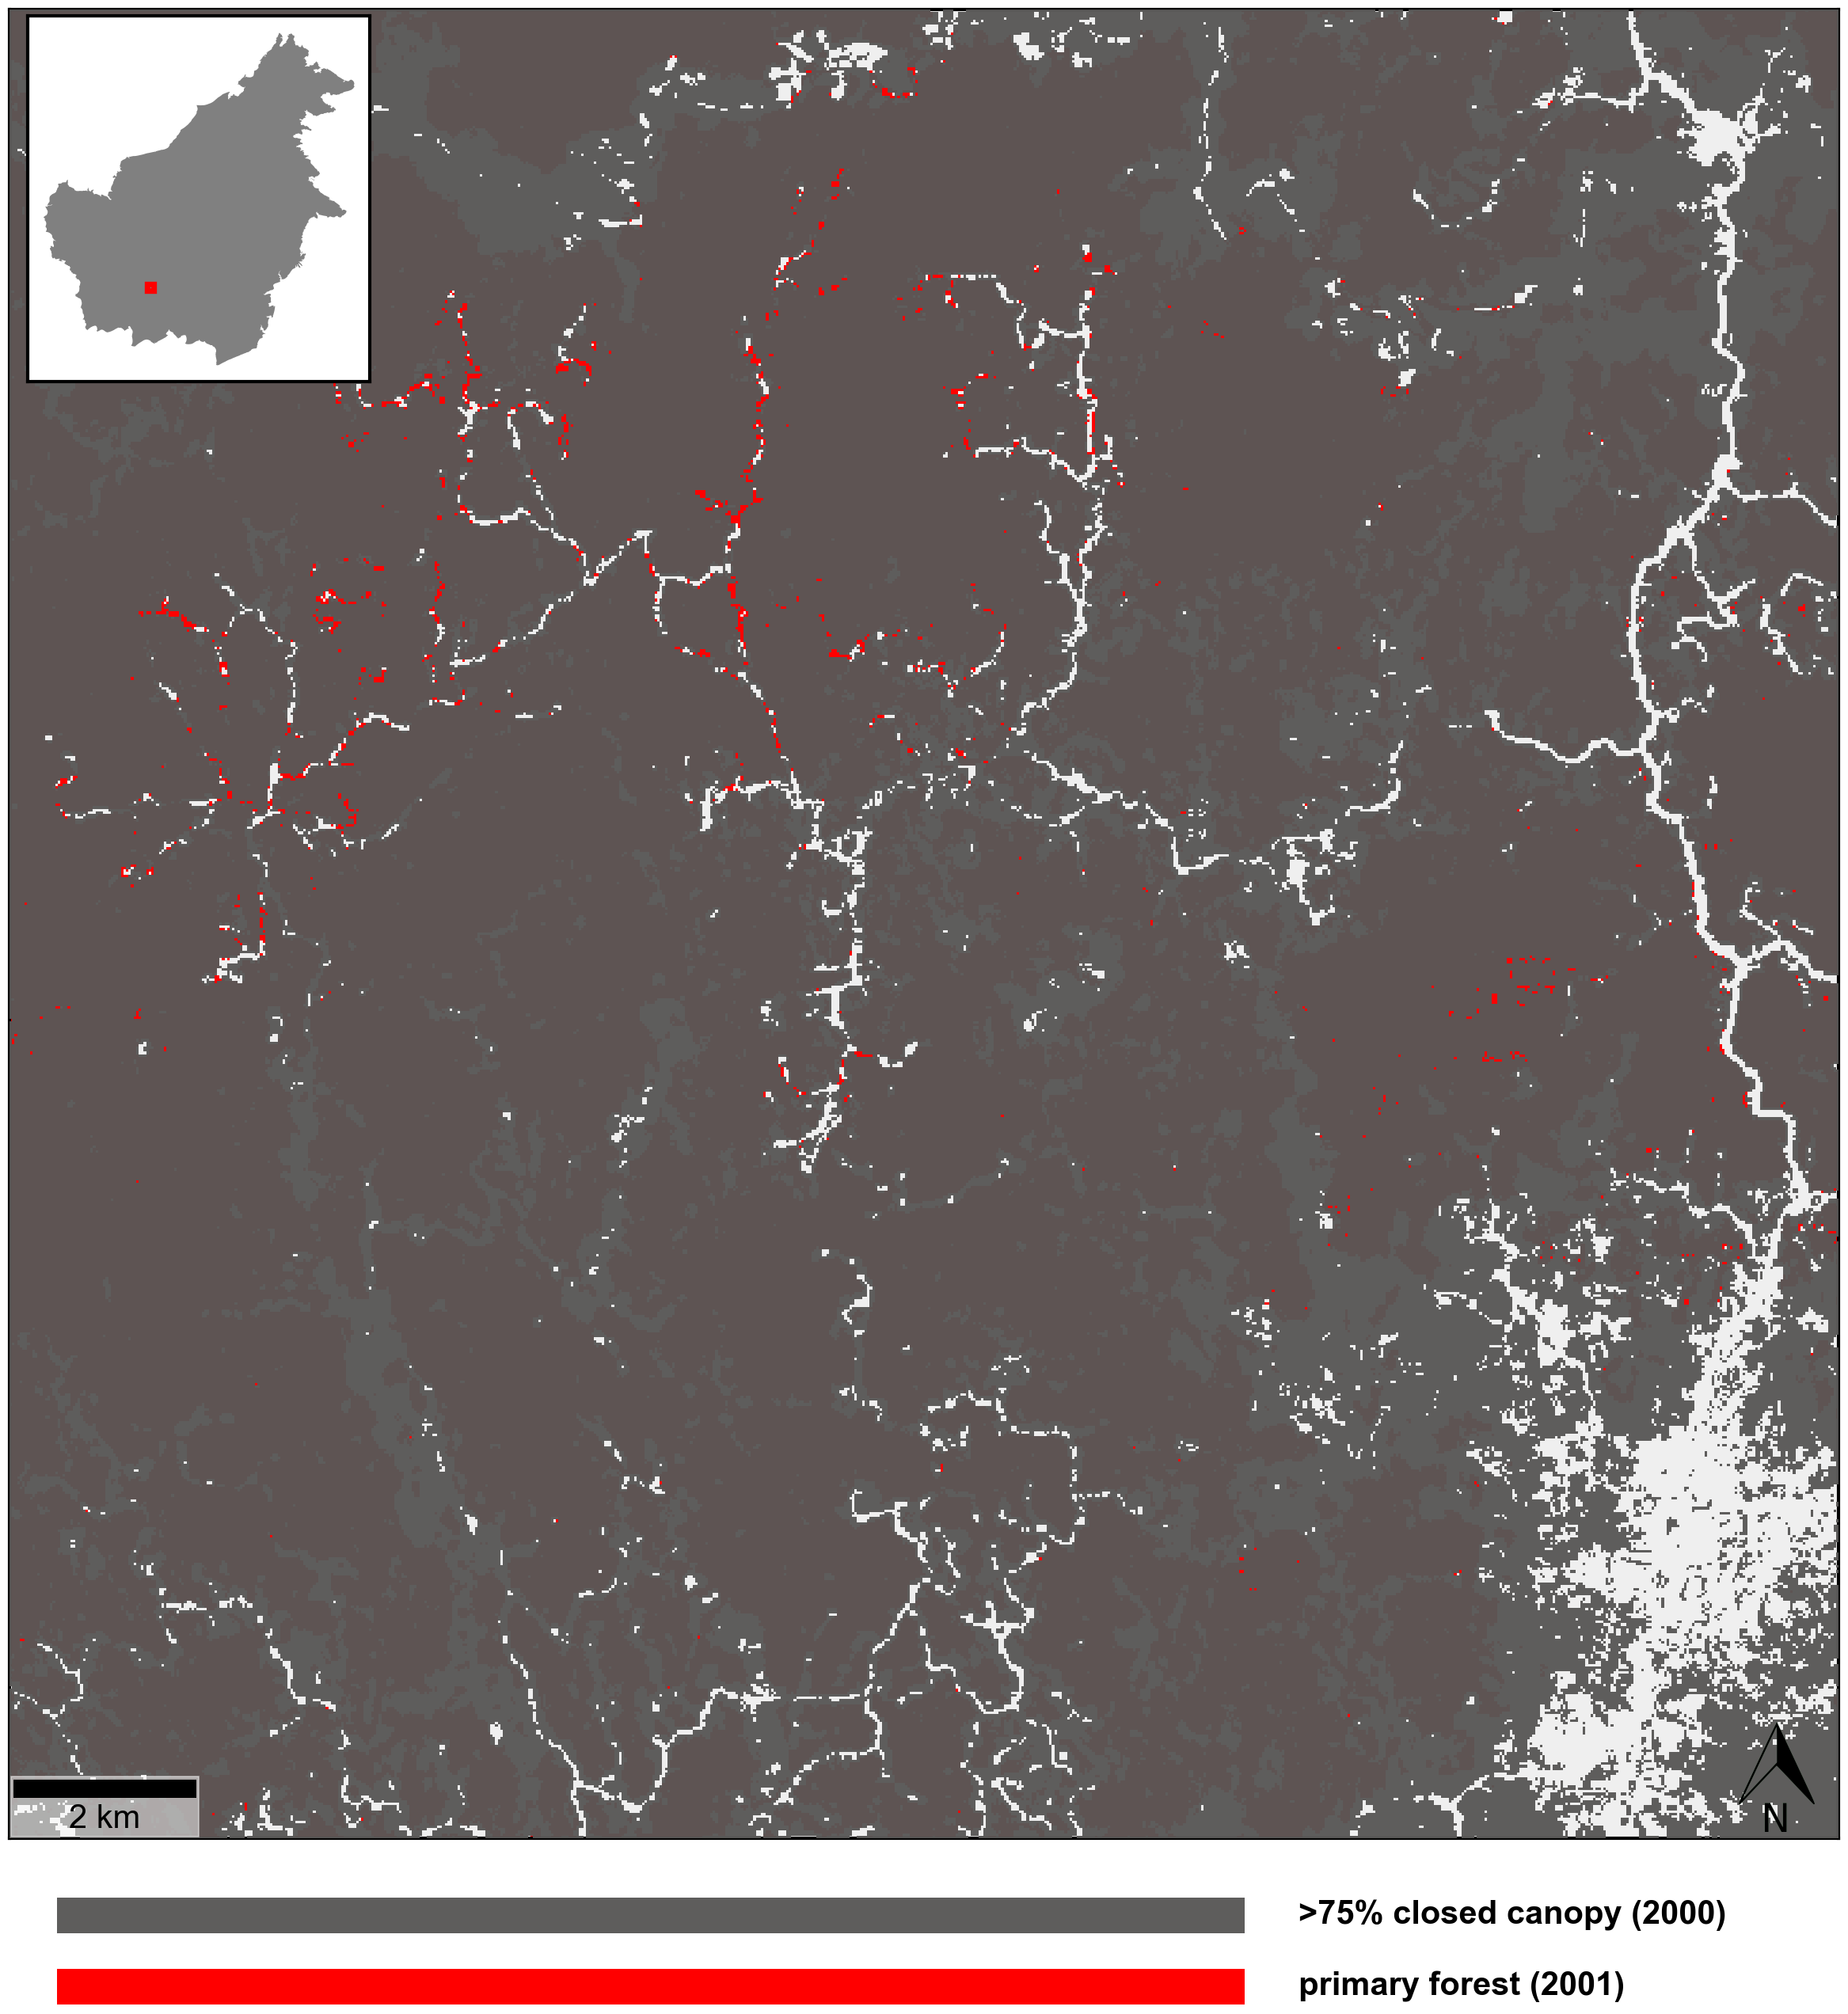
\includegraphics[width=1\textwidth,height=\textheight]{text/../code/results/maps/fcover2000_75_and_primary_forest.png}{]}
\normalcolor

Representative map extract showing that \textgreater75\% closed canopy
of 2000 mostly covers the primary forest of 2001. \newpage

\hypertarget{dense-vegetation-excluding-primary-forests}{%
\section*{\texorpdfstring{\textsc{III} Dense vegetation excluding
primary
forests}{ Dense vegetation excluding primary forests}}\label{dense-vegetation-excluding-primary-forests}}

\markright{\textsc{III} Dense vegetation excluding primary forests}

\color{white}

{[}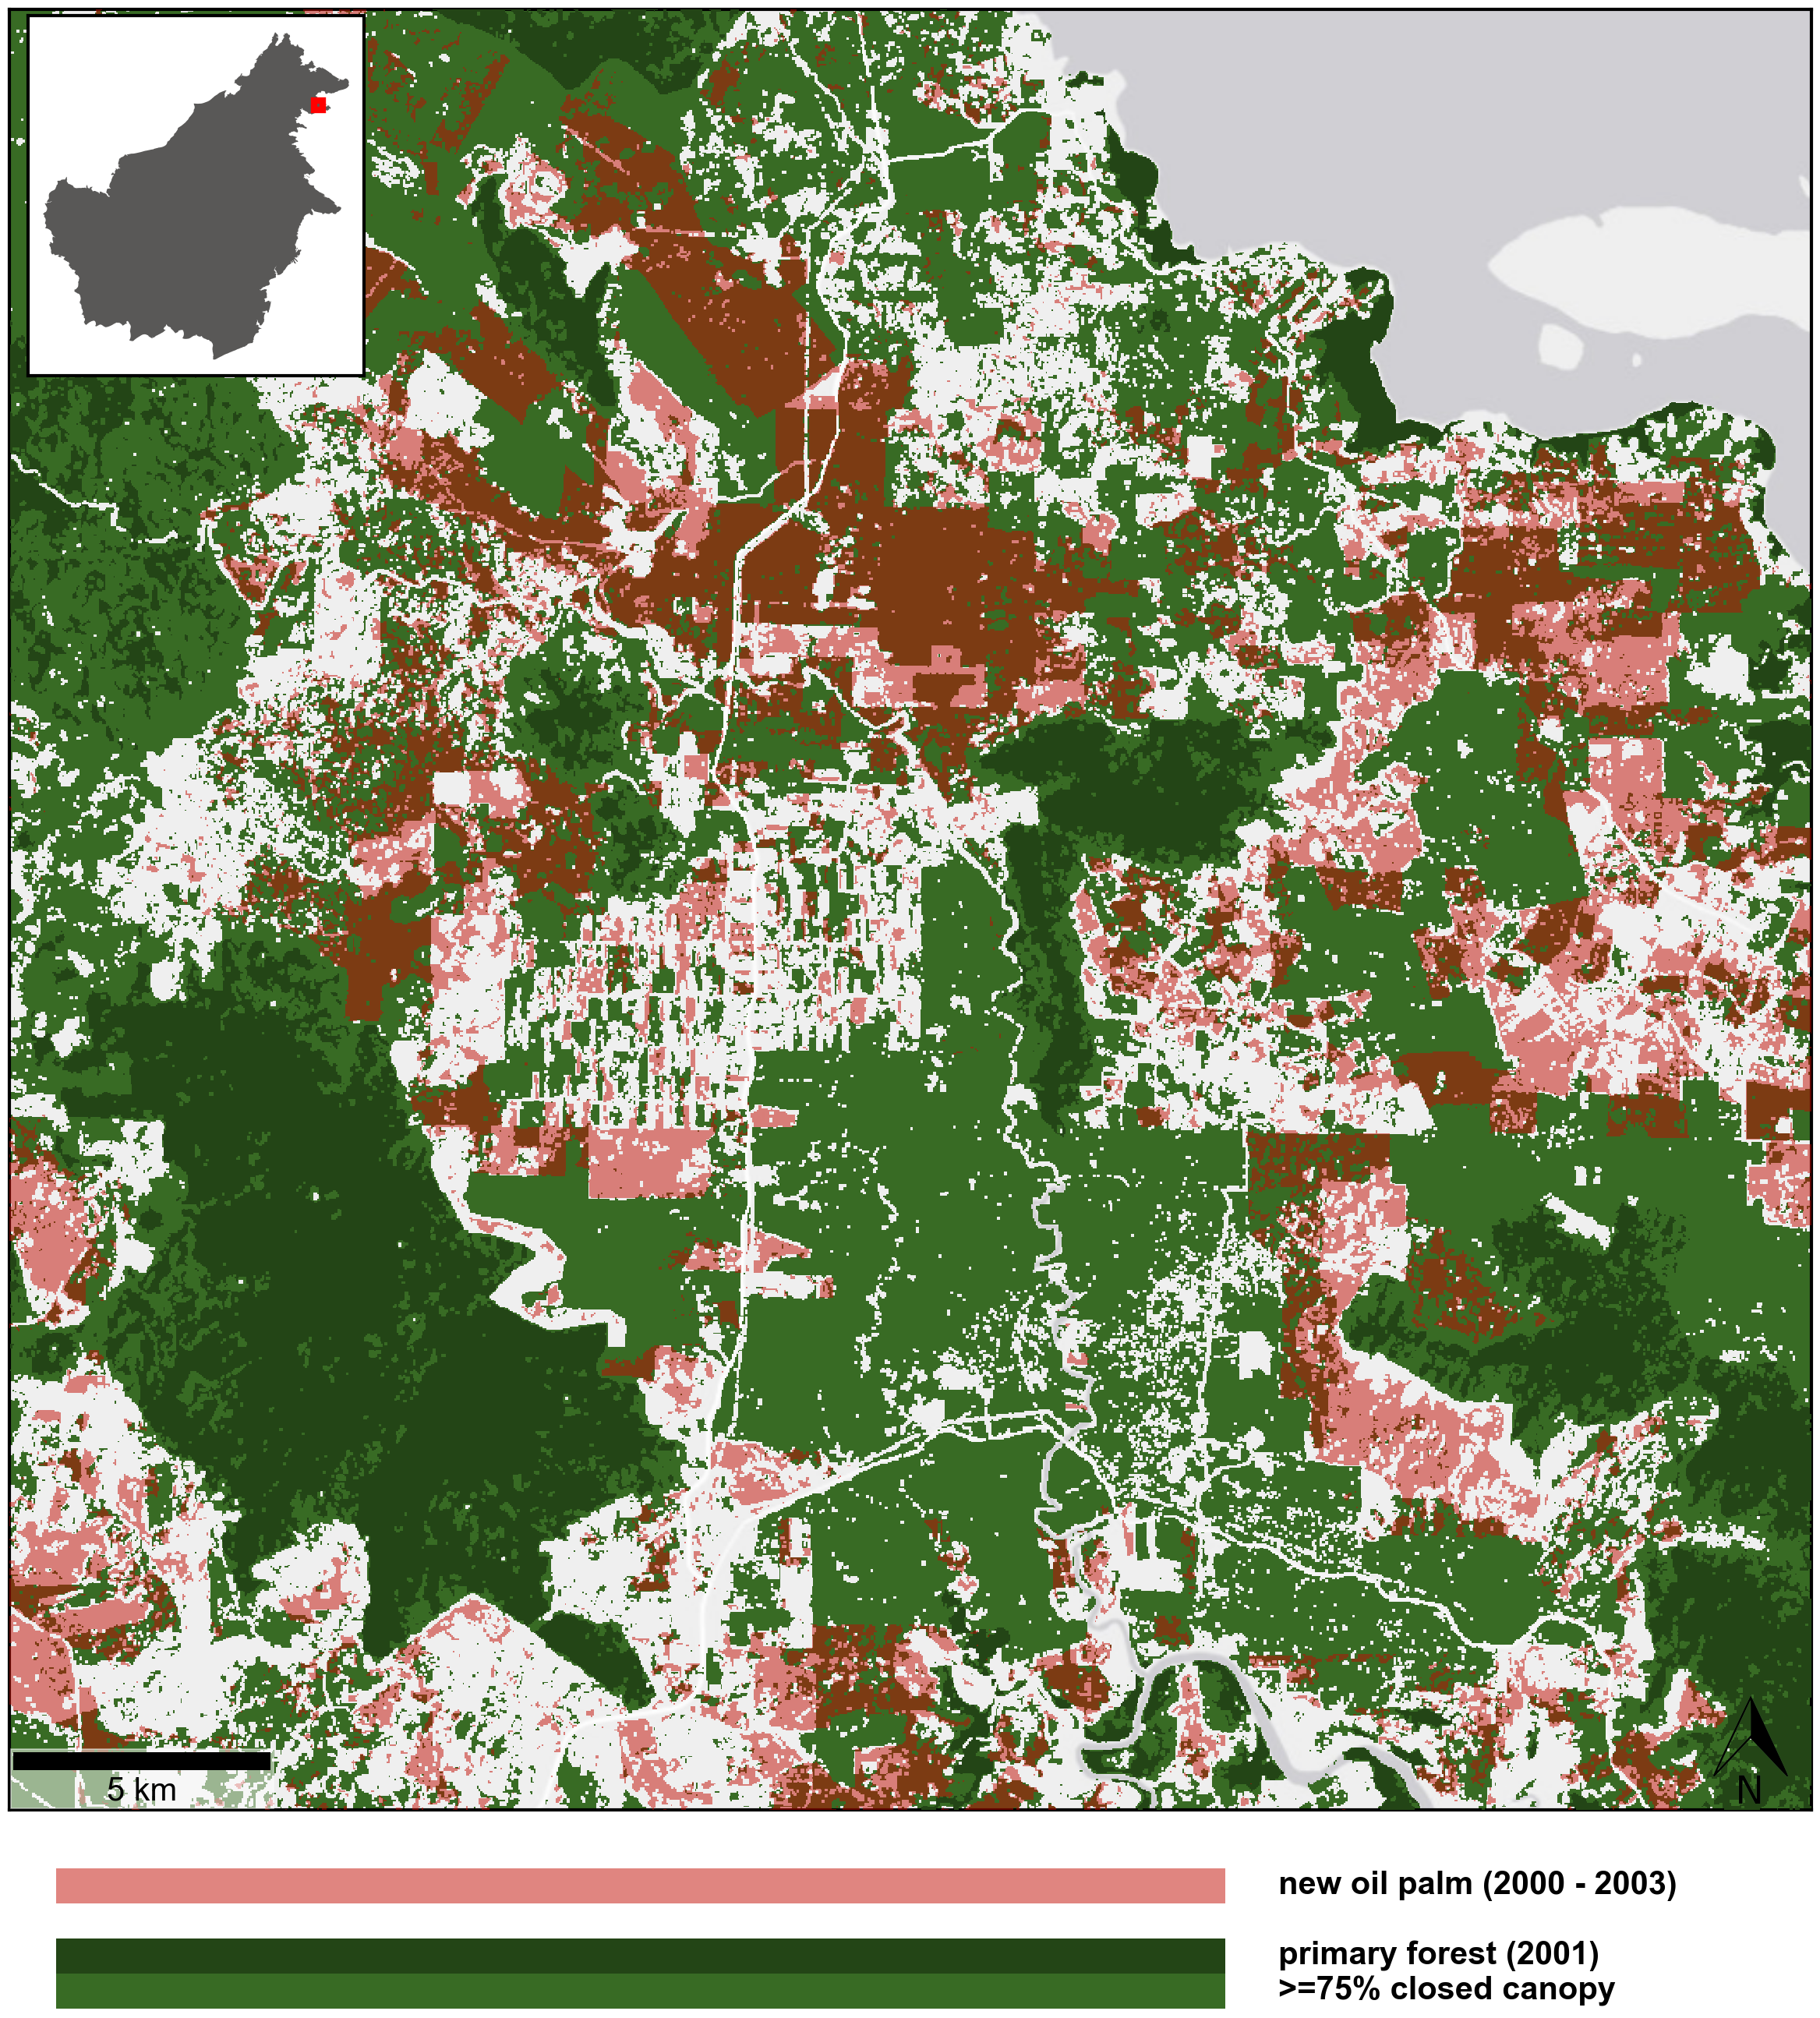
\includegraphics[width=1\textwidth,height=\textheight]{text/../code/results/maps/vegetation_oil_palm_00_03.png}{]}
\normalcolor

In the dense vegetation outside of primary forests, lage areas are
occupied by oil palm. Oil palm data is limited to years 2000 - 2003 as
growing oil palms could alread have a closed canopy of \textgreater75\%
in the year 2000. \newpage

\hypertarget{validation-of-built-up-areas-in-2000-and-deforestation}{%
\section*{\texorpdfstring{\textsc{IV} Validation of built up areas in
2000 and
deforestation}{ Validation of built up areas in 2000 and deforestation}}\label{validation-of-built-up-areas-in-2000-and-deforestation}}

\markright{\textsc{IV} Validation of built up areas in 2000 and
deforestation}

\color{white}

{[}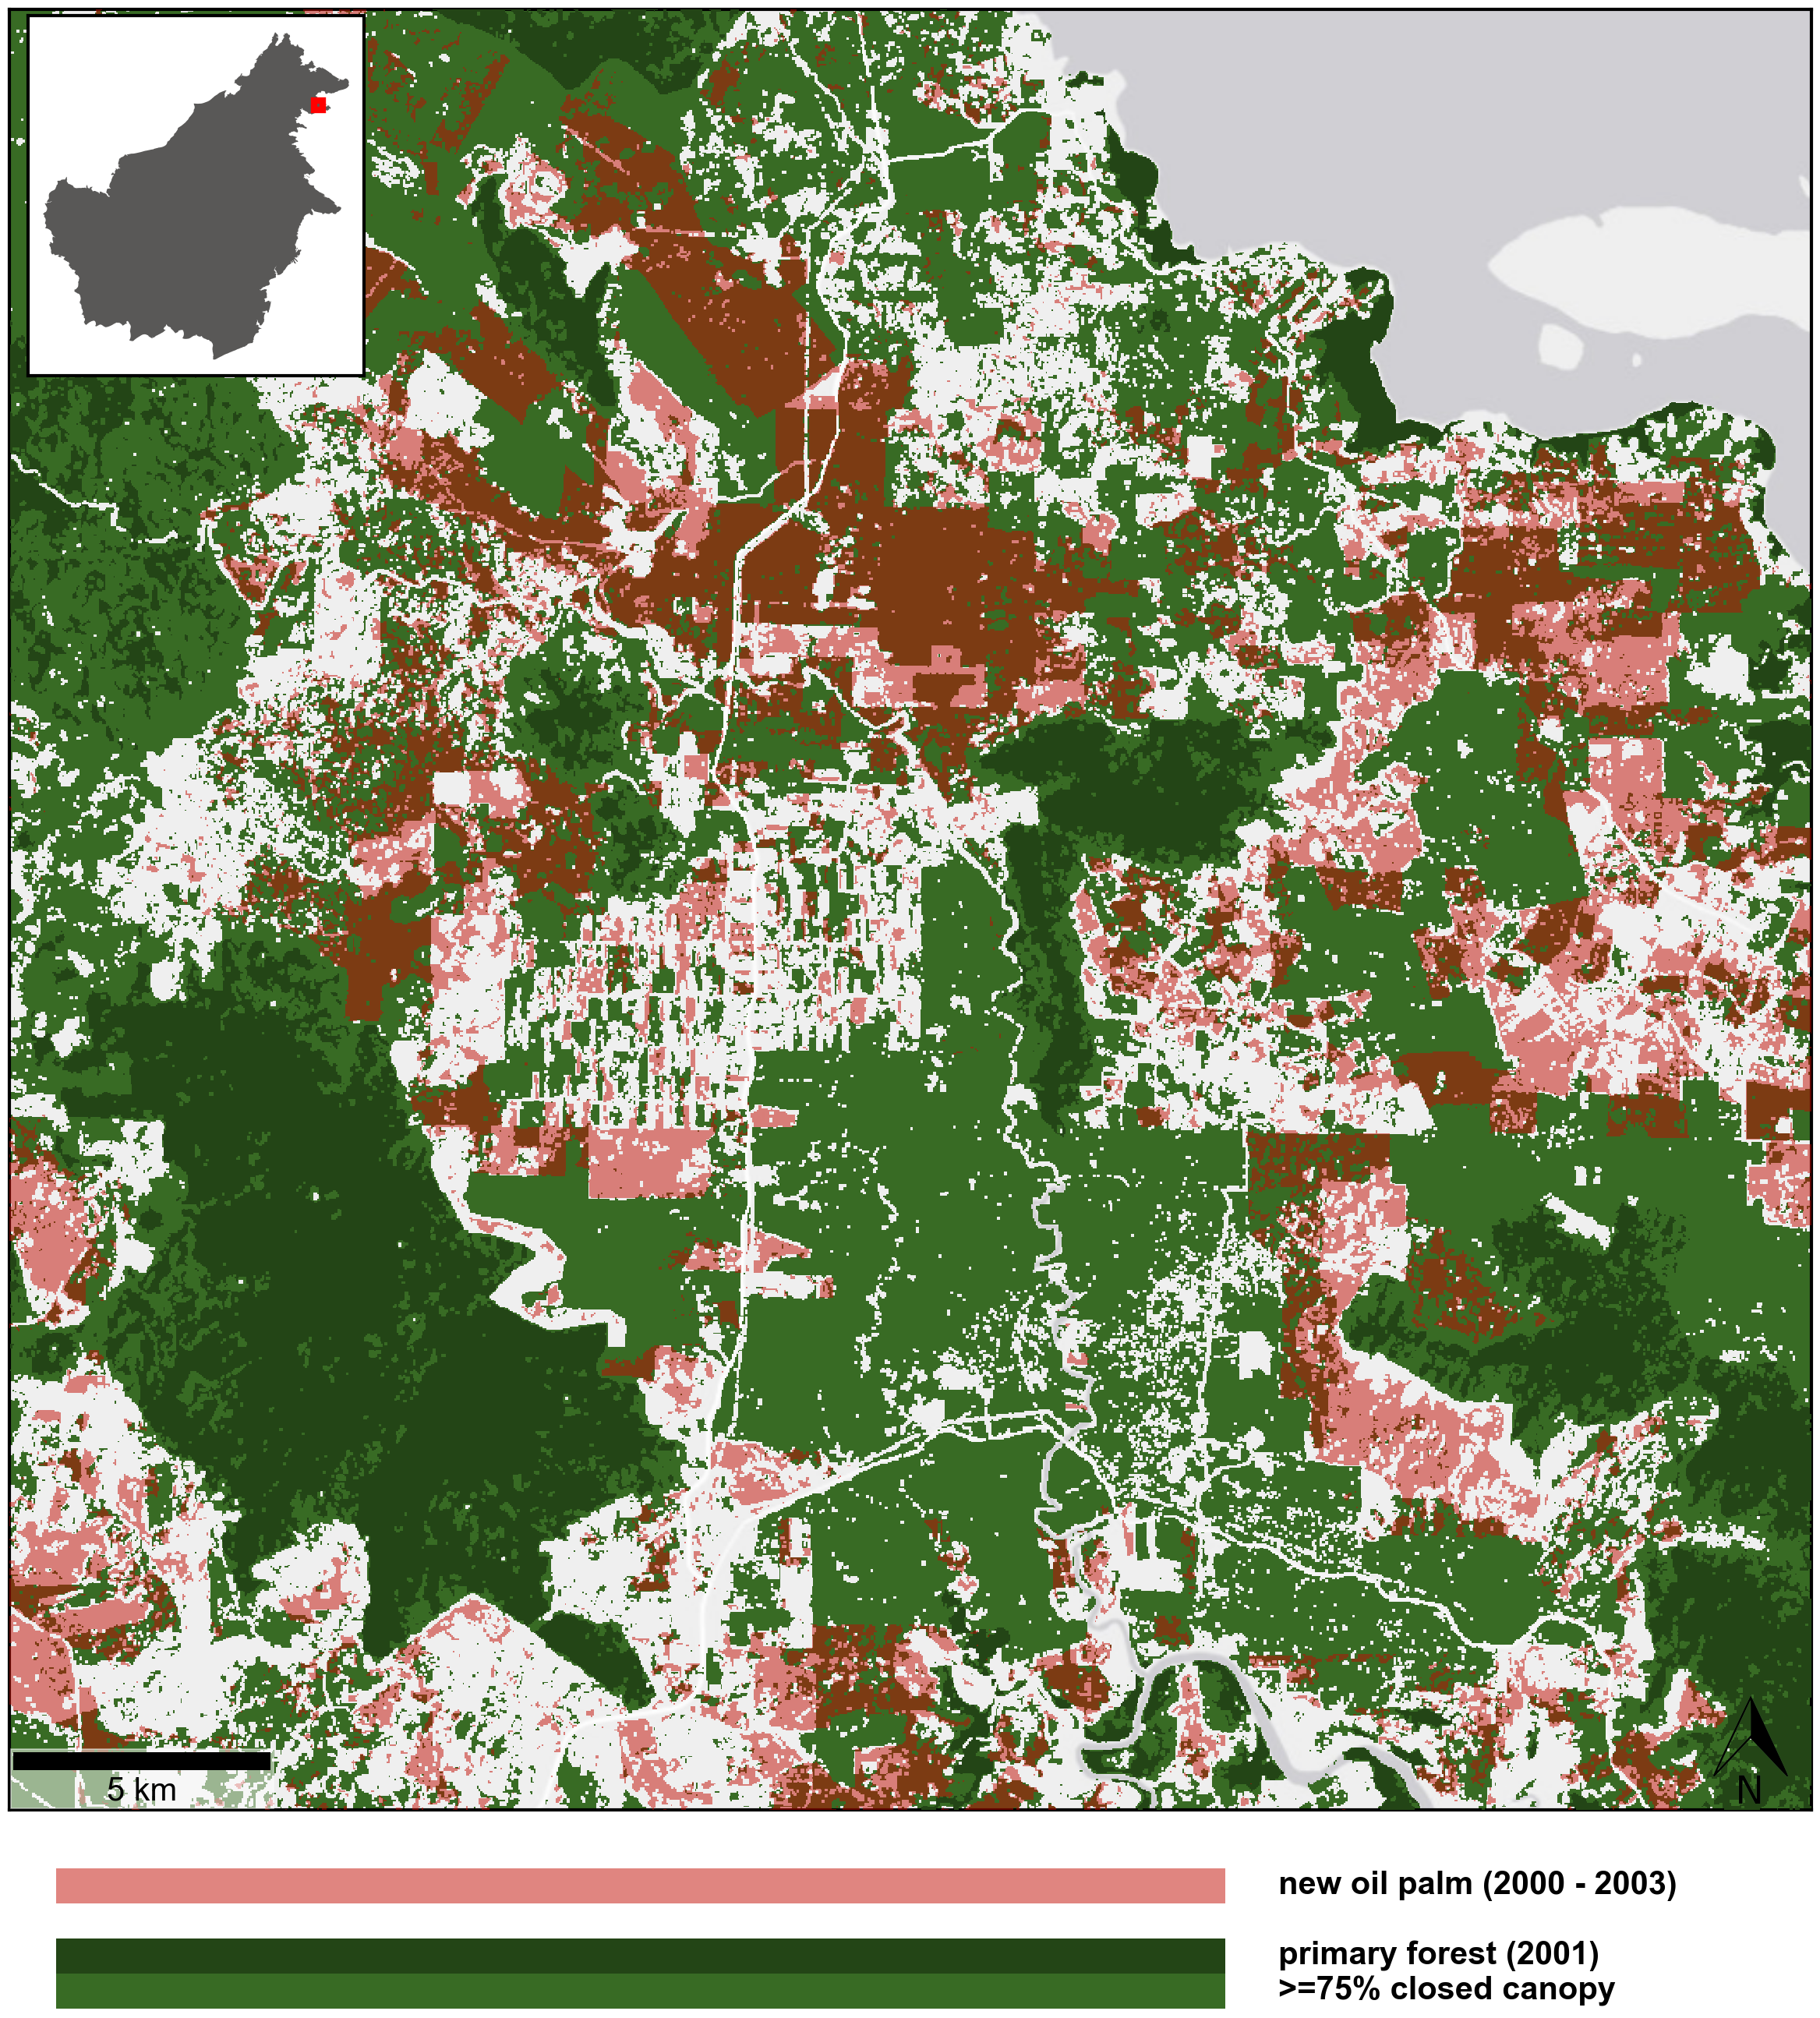
\includegraphics[width=1\textwidth,height=\textheight]{text/../code/results/maps/validation_built_up_deforestation.png}{]}
\normalcolor

Example of deforestation on year 2000 built up area, where, logically,
no deforestation should be. Here it is visible, that these areas are
mainly located at the edge, where maintenance led to the removal of
closeby trees, which were thus classifiead as forest loss. \newpage

\hypertarget{secondary-forest-and-proximity-to-rivers}{%
\section*{\texorpdfstring{\textsc{V} Secondary Forest and proximity to
rivers}{ Secondary Forest and proximity to rivers}}\label{secondary-forest-and-proximity-to-rivers}}

\markright{\textsc{V} Secondary Forest and proximity to rivers}

\color{white}

{[}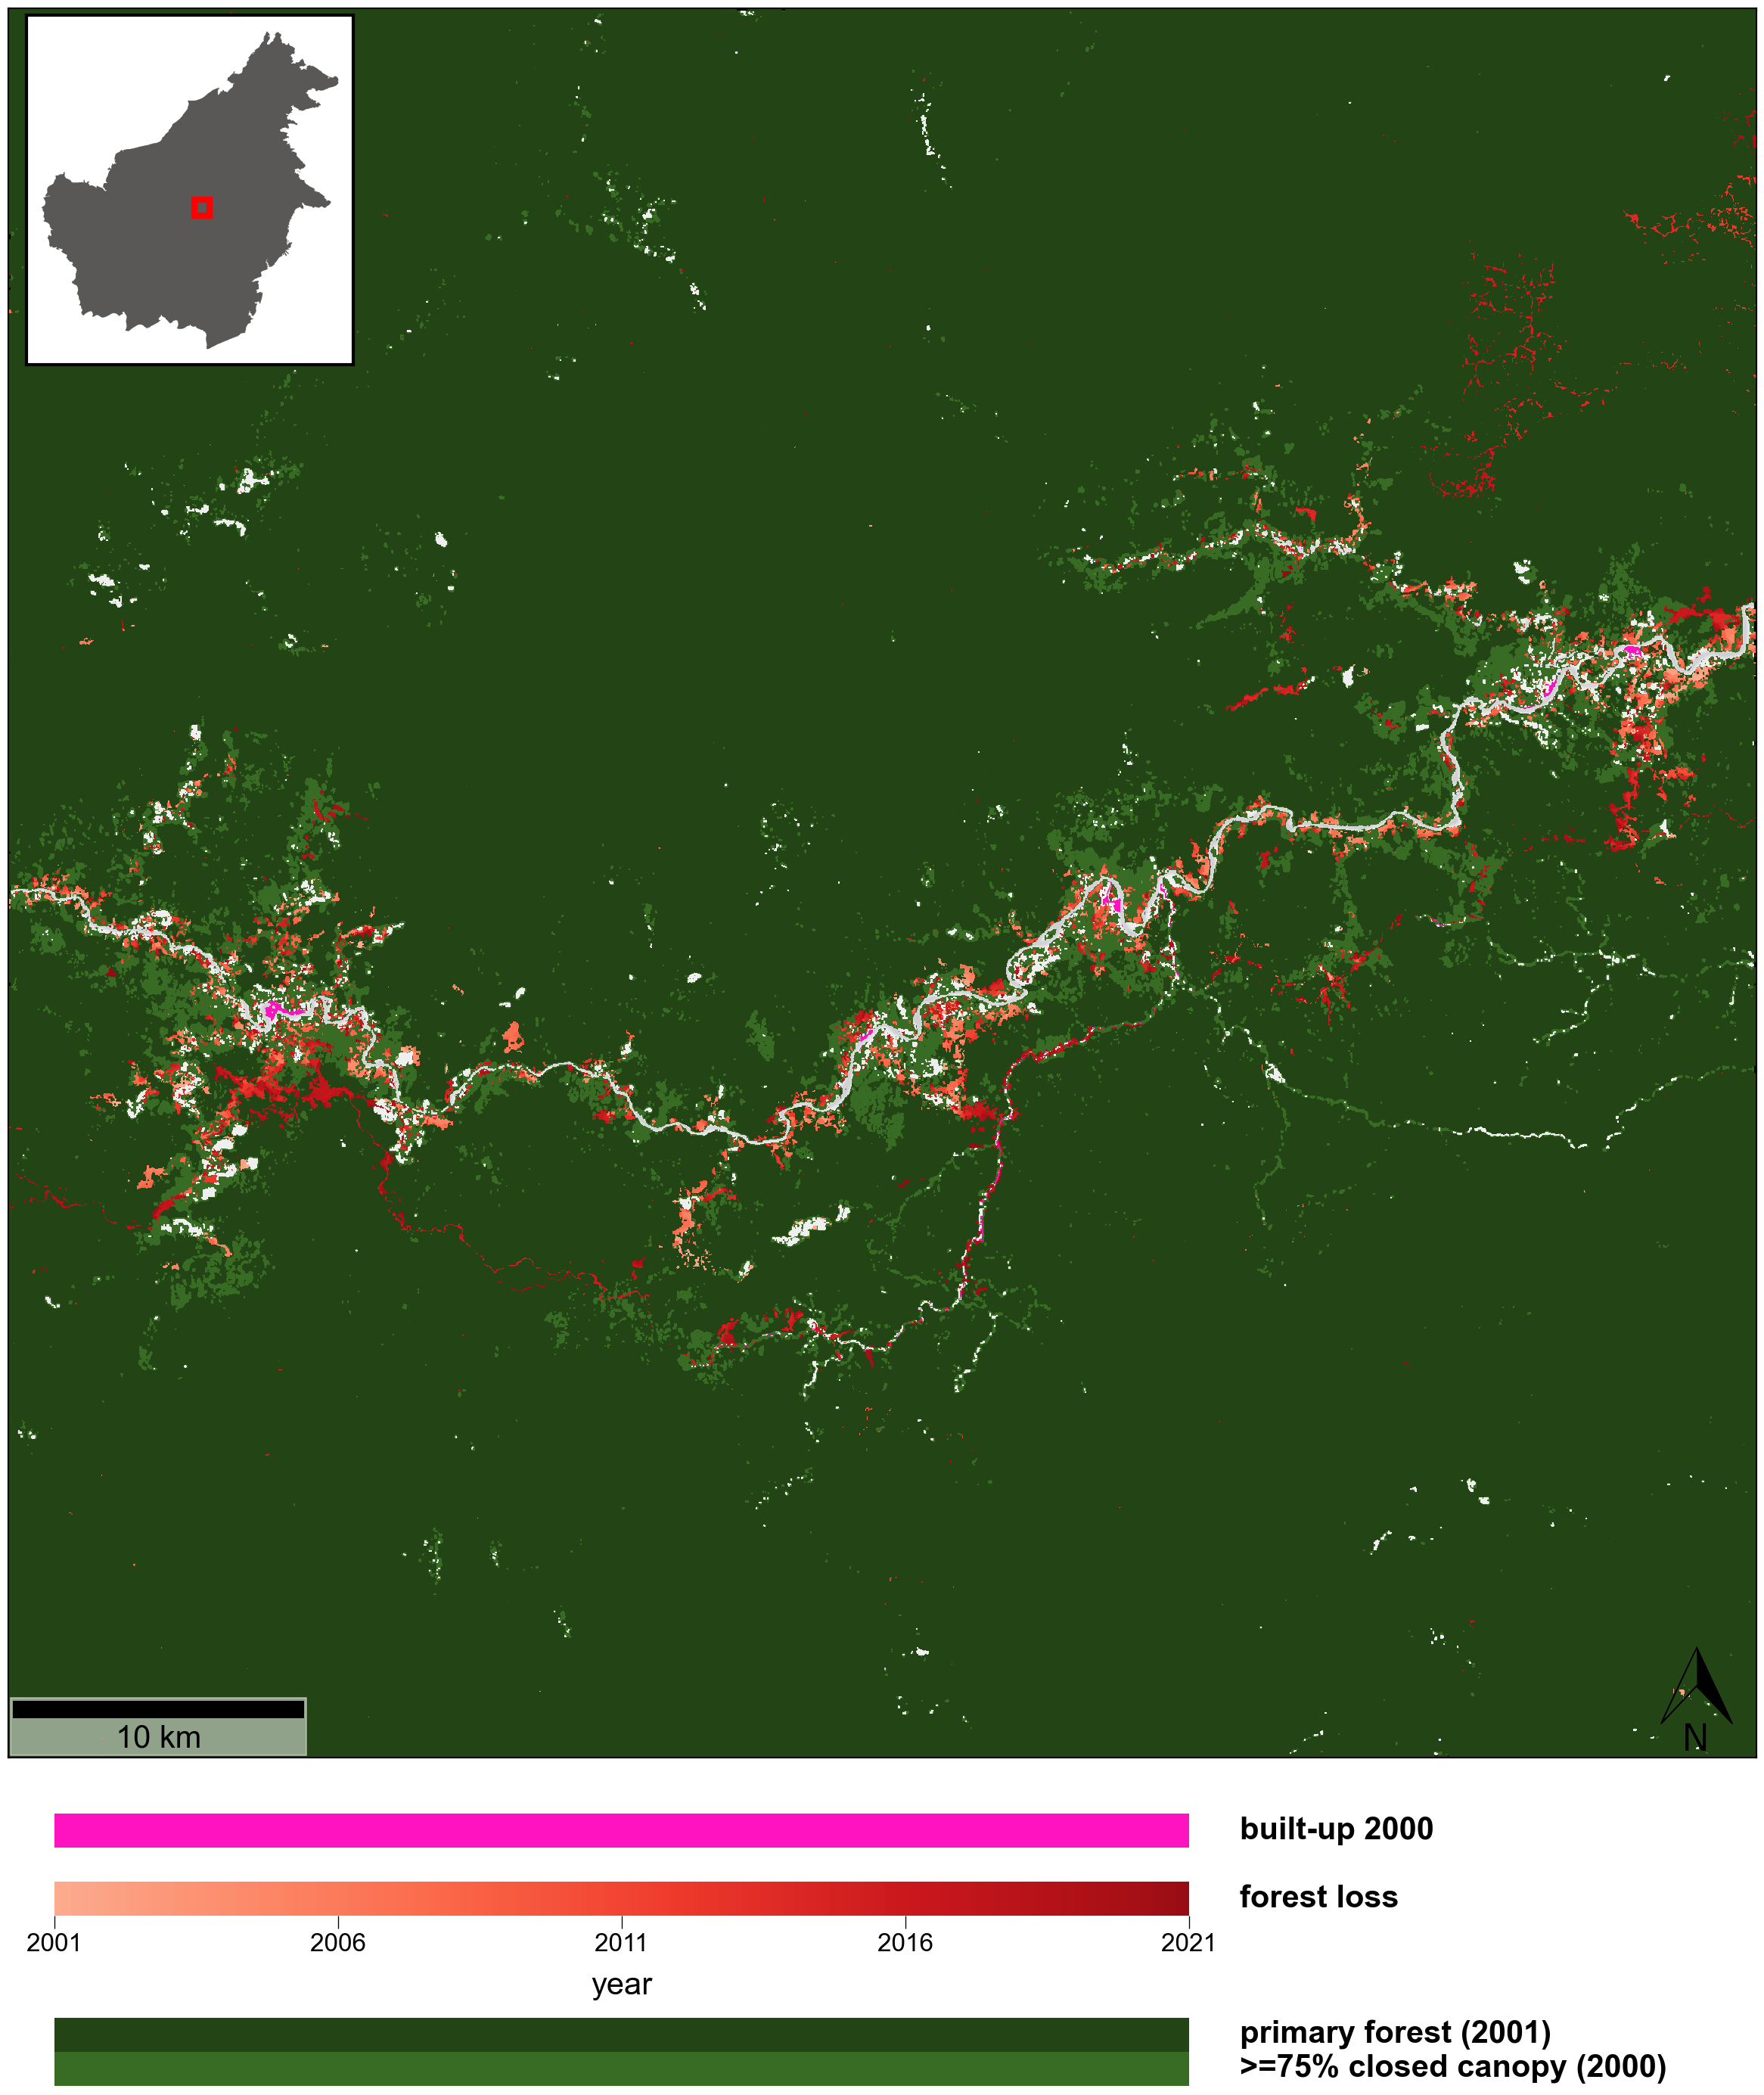
\includegraphics[width=1\textwidth,height=\textheight]{text/../code/results/maps/reason_secondary_rivers.png}{]}
\normalcolor

A repeating pattern, with a lot of secondary forest close to rivers,
especially with built-up areas nearby. \newpage

\hypertarget{logging-in-pas}{%
\section*{\texorpdfstring{\textsc{VI} Logging in
PAs}{ Logging in PAs}}\label{logging-in-pas}}

\markright{\textsc{VI} Logging in PAs}

\color{white}

{[}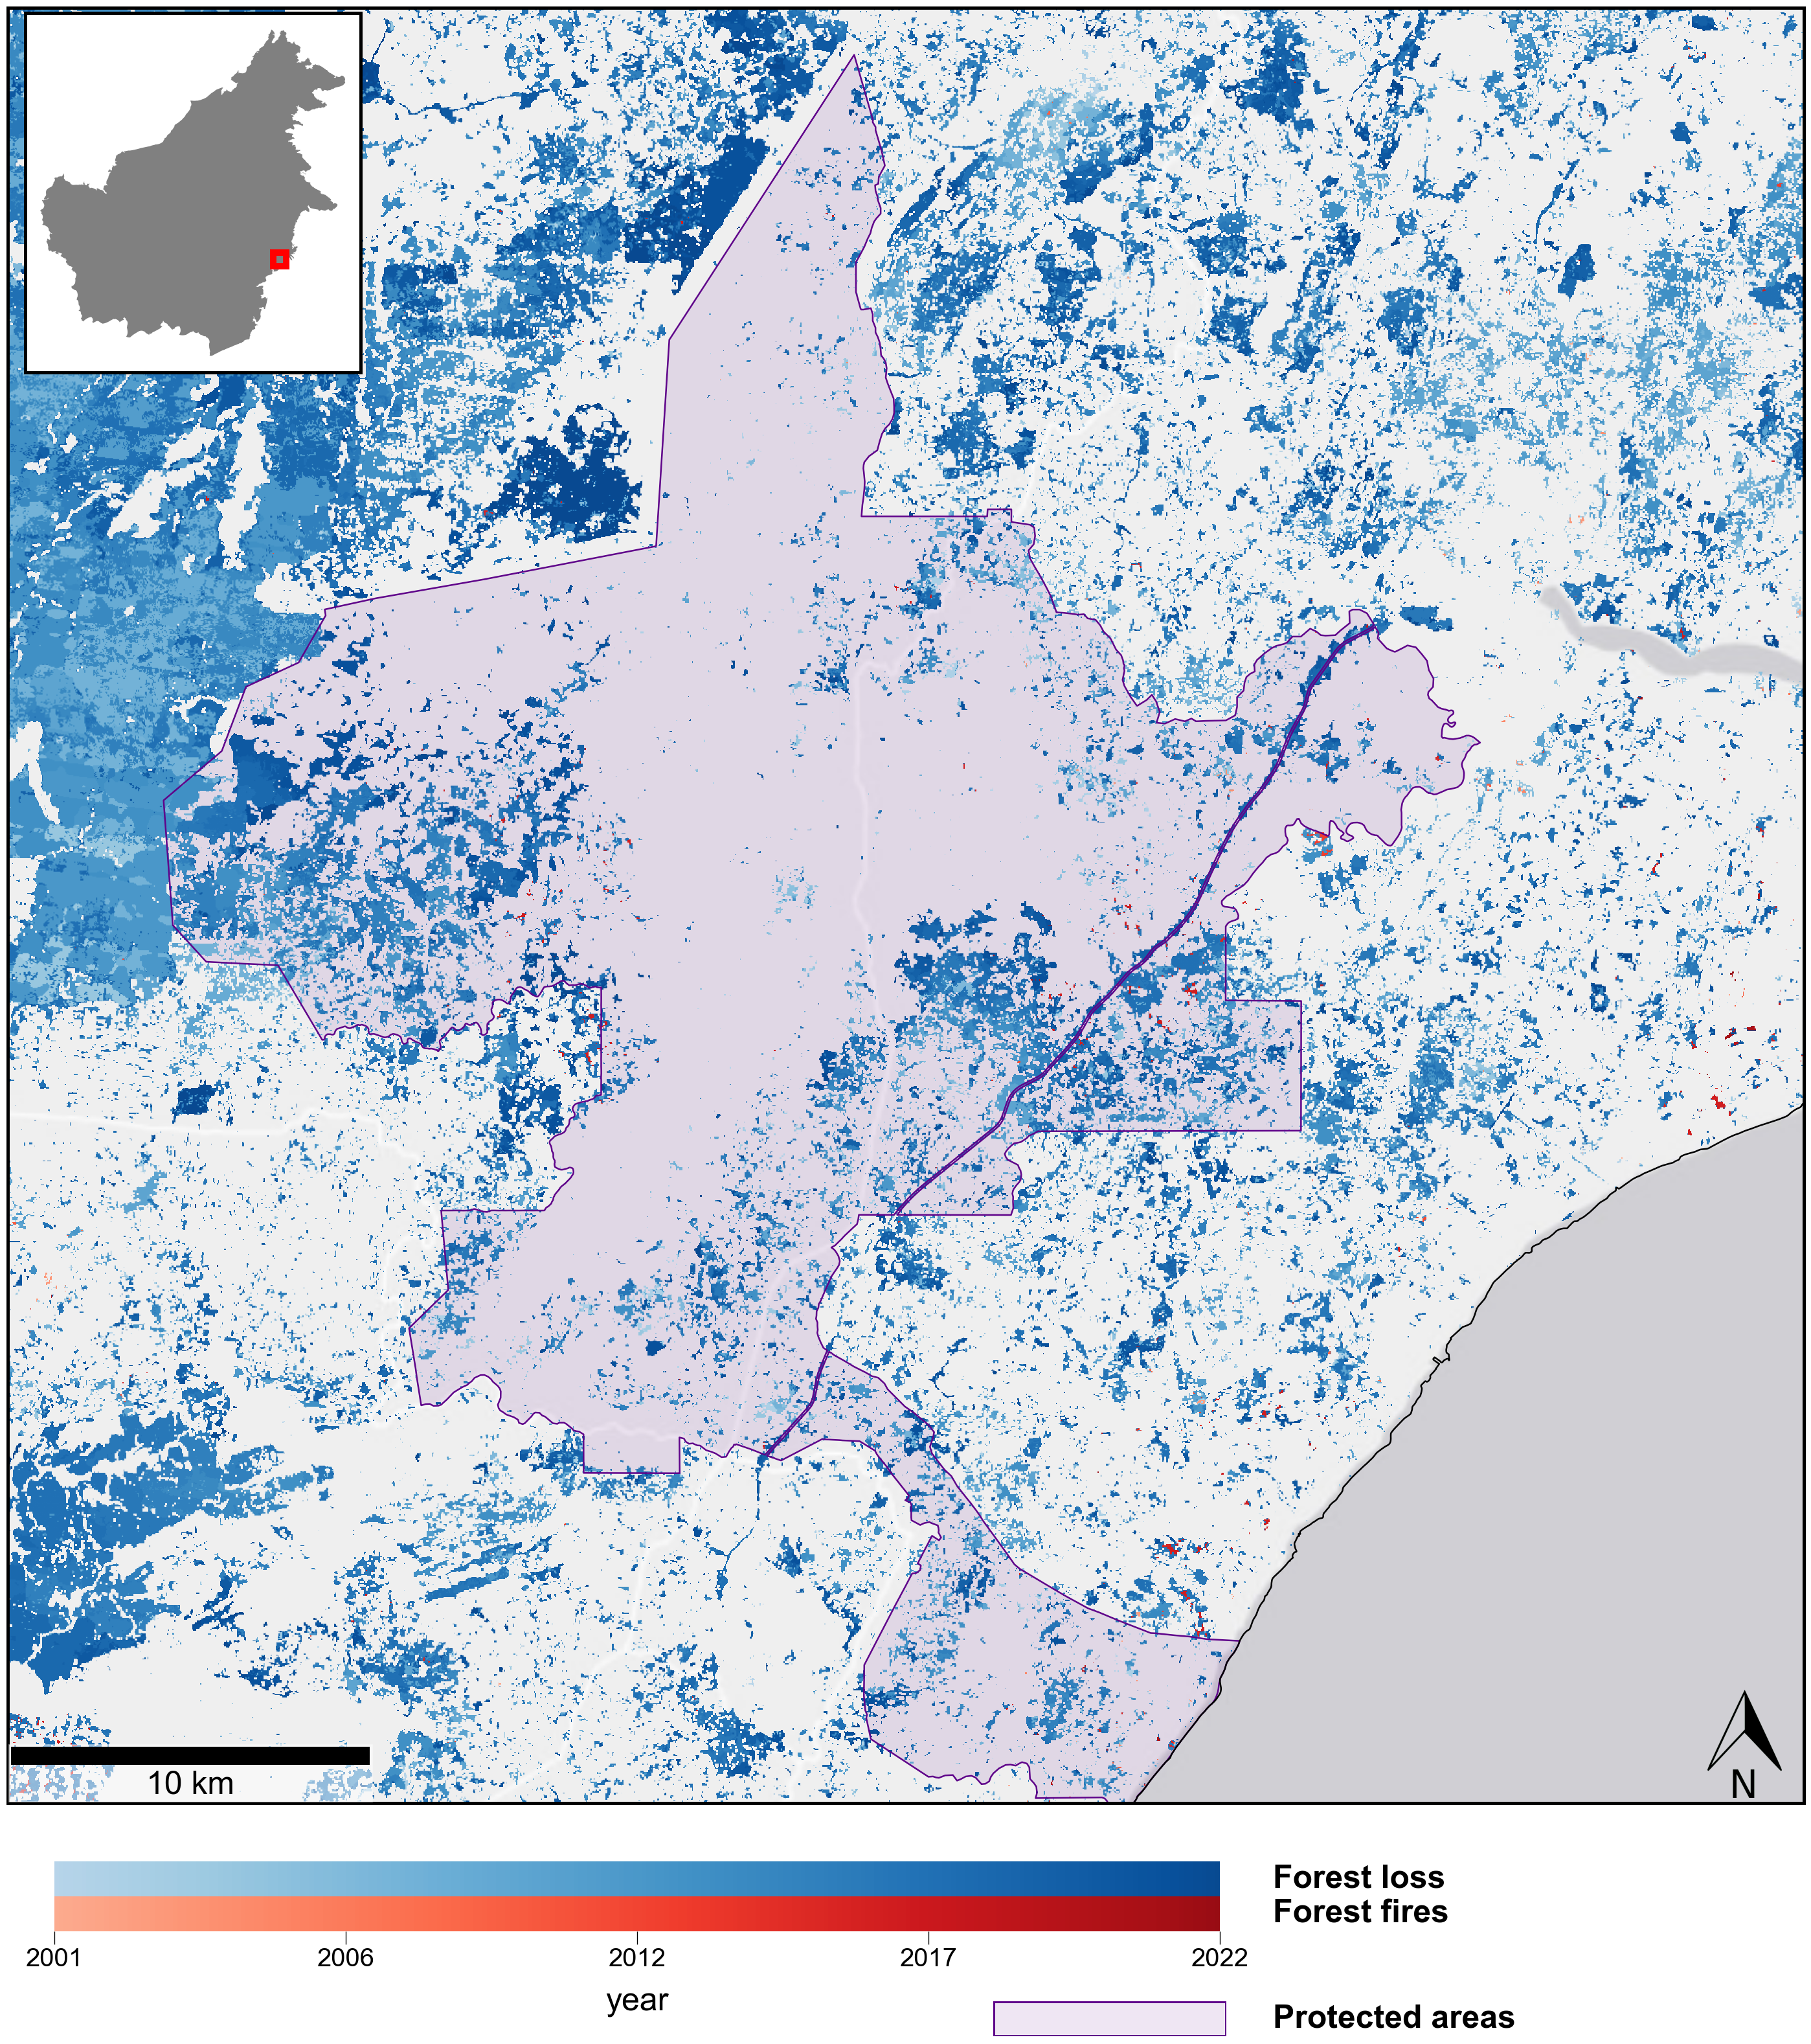
\includegraphics[width=1\textwidth,height=\textheight]{text/../code/results/maps/deforestation_protected_areas_other.png}{]}
\normalcolor

An exceptional case of a protected PA where much deforestation takes
place. A prominent feature is a new road that cuts through the PA.
\newpage

\hypertarget{socondary-forest-loss-in-rspo-concessions}{%
\section*{\texorpdfstring{\textsc{VII} Socondary forest loss in RSPO
concessions}{ Socondary forest loss in RSPO concessions}}\label{socondary-forest-loss-in-rspo-concessions}}

\markright{\textsc{VII} Socondary forest loss in RSPO concessions}

\color{white}

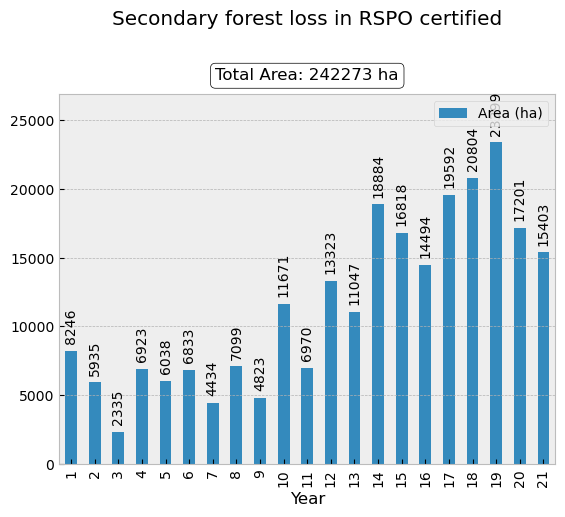
\includegraphics[width=0.65\textwidth,height=\textheight]{text/../code/results/plots/RSPO_secondary_forest_loss.png}

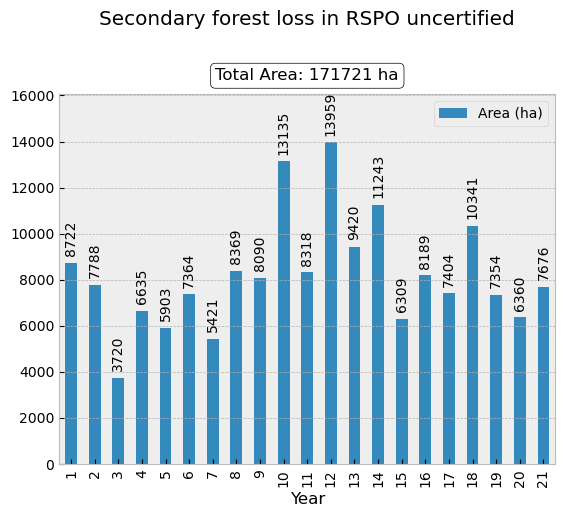
\includegraphics[width=0.65\textwidth,height=\textheight]{text/../code/results/plots/RSPO_secondary_forest_loss_uncertified.png}

\normalcolor

Elevated levels of secondary forest loss in RSPO certified concessions
and continuous loss in uncertified concessions.

\newpage

\hypertarget{oill-palm-after-forest-fies}{%
\section*{\texorpdfstring{\textsc{IX} Oill palm after forest
fies}{ Oill palm after forest fies}}\label{oill-palm-after-forest-fies}}

\markright{\textsc{IX} Oill palm after forest fies}

\color{white}

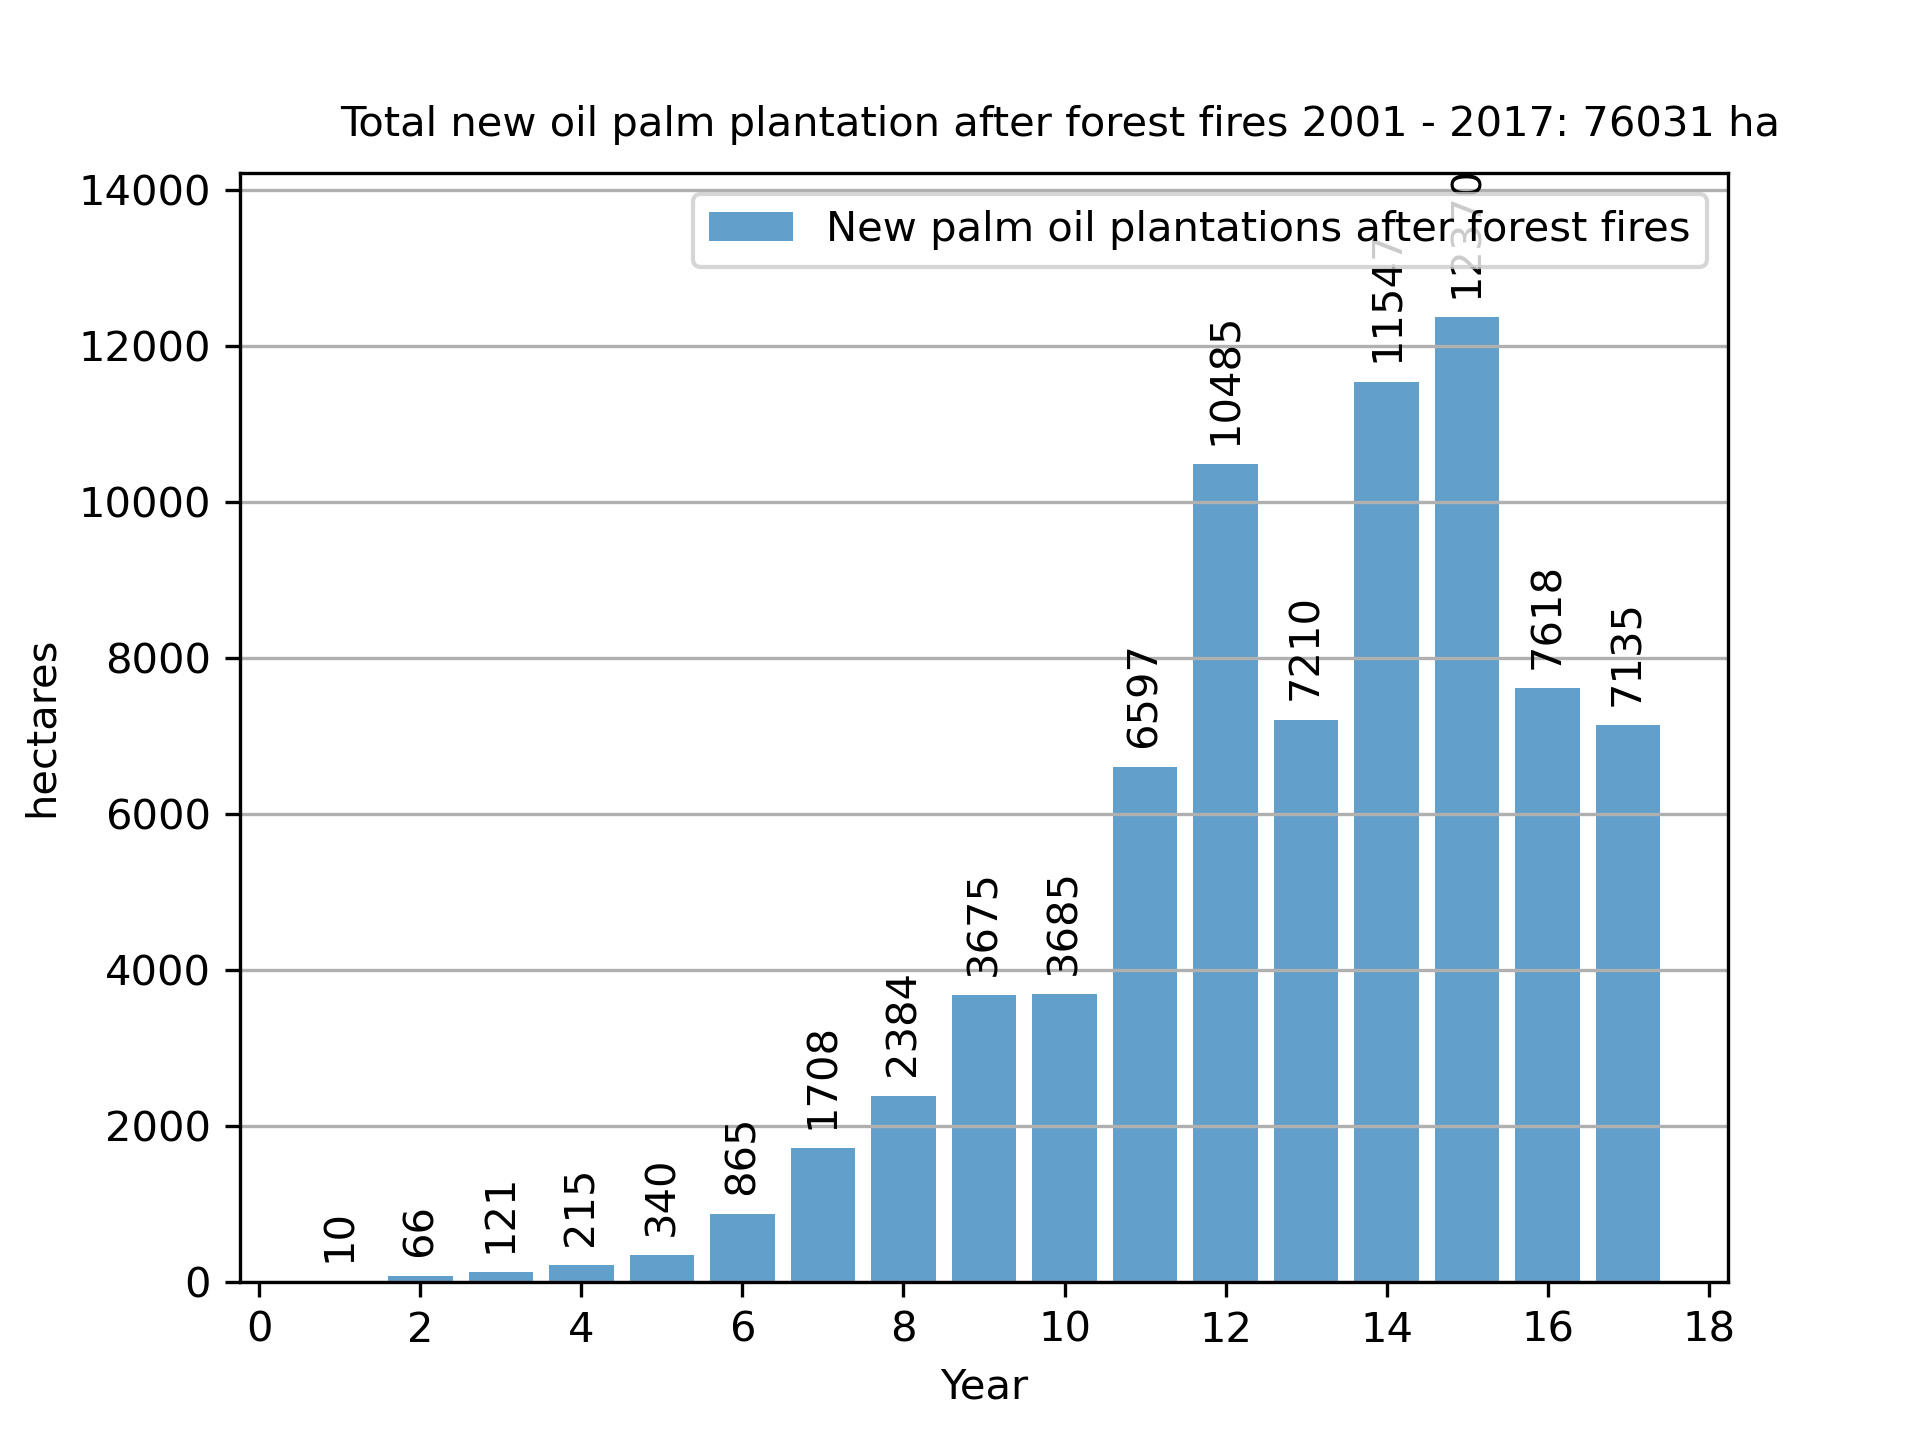
\includegraphics[width=0.5\textwidth,height=\textheight]{text/../code/results/final_plots/new_oil_palm_after_forest_fires.png}
\normalcolor

Typical deforestation patterns in eastern Borneo with a few large areas
of deforestation inland, smaller scale near the coast, and a clear
delineation to protected area with very little forest loss.

\newpage

\hypertarget{sec-annex_x}{%
\section*{\texorpdfstring{\textsc{X} Plagiarism
declaration}{ Plagiarism declaration}}\label{sec-annex_x}}

\markright{\textsc{X} Plagiarism declaration}

\color{white}

{[}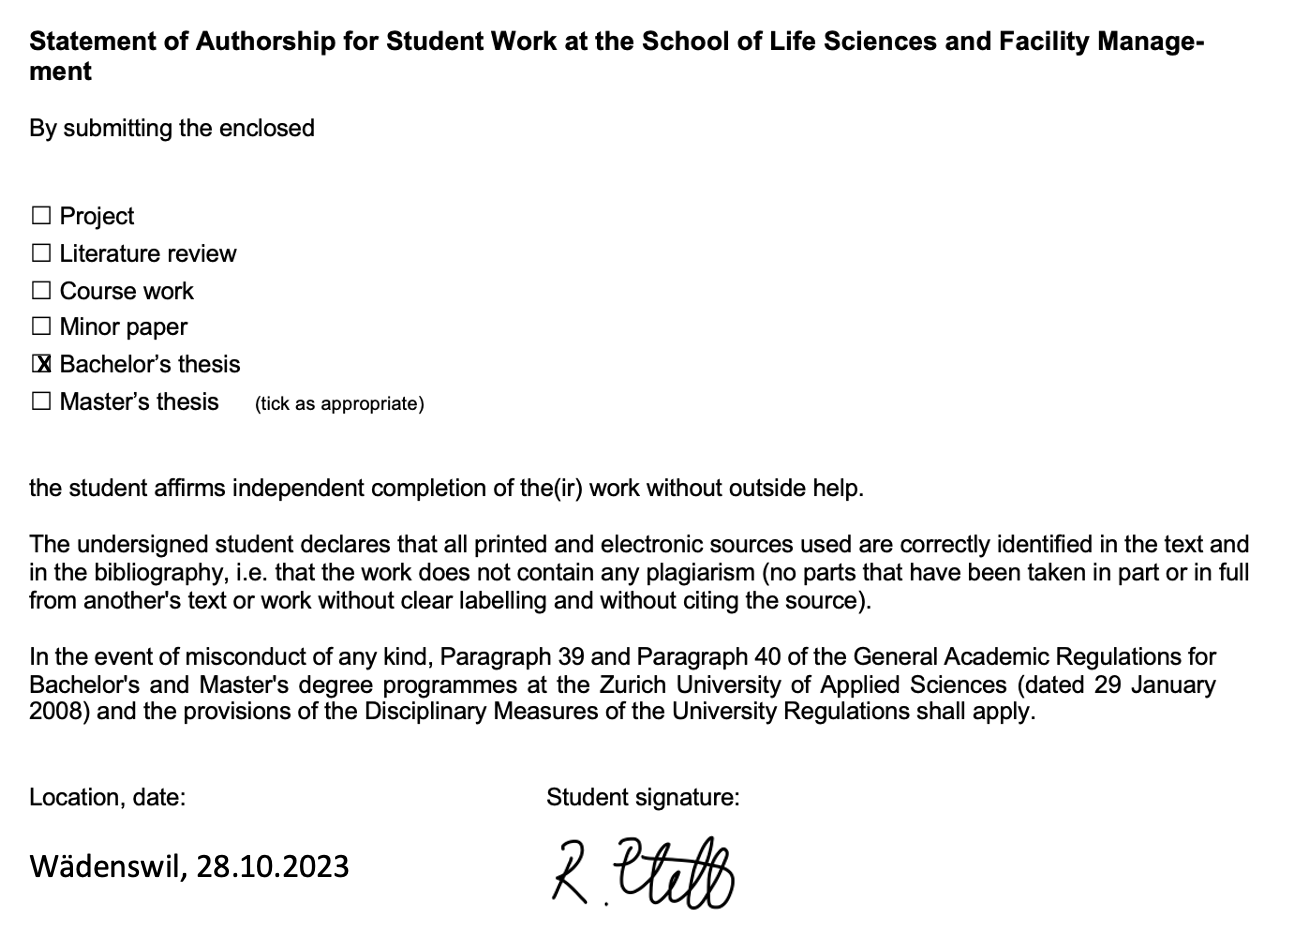
\includegraphics[width=1\textwidth,height=\textheight]{text/annex_files/plagiarism_declaration.png}{]}
\normalcolor \newpage



\end{document}
